
\paragraph{Module inventory rule.} This section is a generated repository view, not a second planning source. It is derived from the frozen SM9h Lean source snapshot by \texttt{scripts/build\_export\_script\_v1.8.py}. The planning YAML remains the only manually maintained roadmap source; the module catalog, dependency summaries, source-path links, and graph figures are regenerated from the repository snapshot.
\subsection*{Inventory summary}
\small
\arrayrulecolor{black!22}
\begin{longtable}{L{0.26\linewidth} L{0.7\linewidth}}
\hline
\textbf{Metric} & \textbf{Value}\\
\hline
\endfirsthead
\hline
\textbf{Metric} & \textbf{Value}\\
\hline
\endhead
Lean modules & 287\\
\hline
\addlinespace[0.24em]
Internal import edges & 724\\
\hline
\addlinespace[0.24em]
External import edges & 43\\
\hline
\addlinespace[0.24em]
Missing internal imports & 0\\
\hline
\addlinespace[0.24em]
Import graph acyclic & True\\
\hline
\addlinespace[0.24em]
Symbol declarations detected & 8366\\
\hline
\addlinespace[0.24em]
Symbol-reference edges detected & 372\\
\hline
\addlinespace[0.24em]
Architectural core modules & 241\\
\hline
\addlinespace[0.24em]
Artifact/\allowbreak{}build/\allowbreak{}notation/\allowbreak{}top-level modules & 46\\
\hline
\addlinespace[0.24em]
\end{longtable}
\arrayrulecolor{black}
\normalsize

\subsection*{Module dependency graphs}
\subsection*{Graph A: group-level import/dependency overview}
\paragraph{Arrow convention.} An edge \(A \to B\) means that at least one module in group \(A\) imports or depends on a module in group \(B\). The arrow points from the importing/consuming group to the required dependency. This is a technical import graph, not a semantic derivation graph.
\begin{center}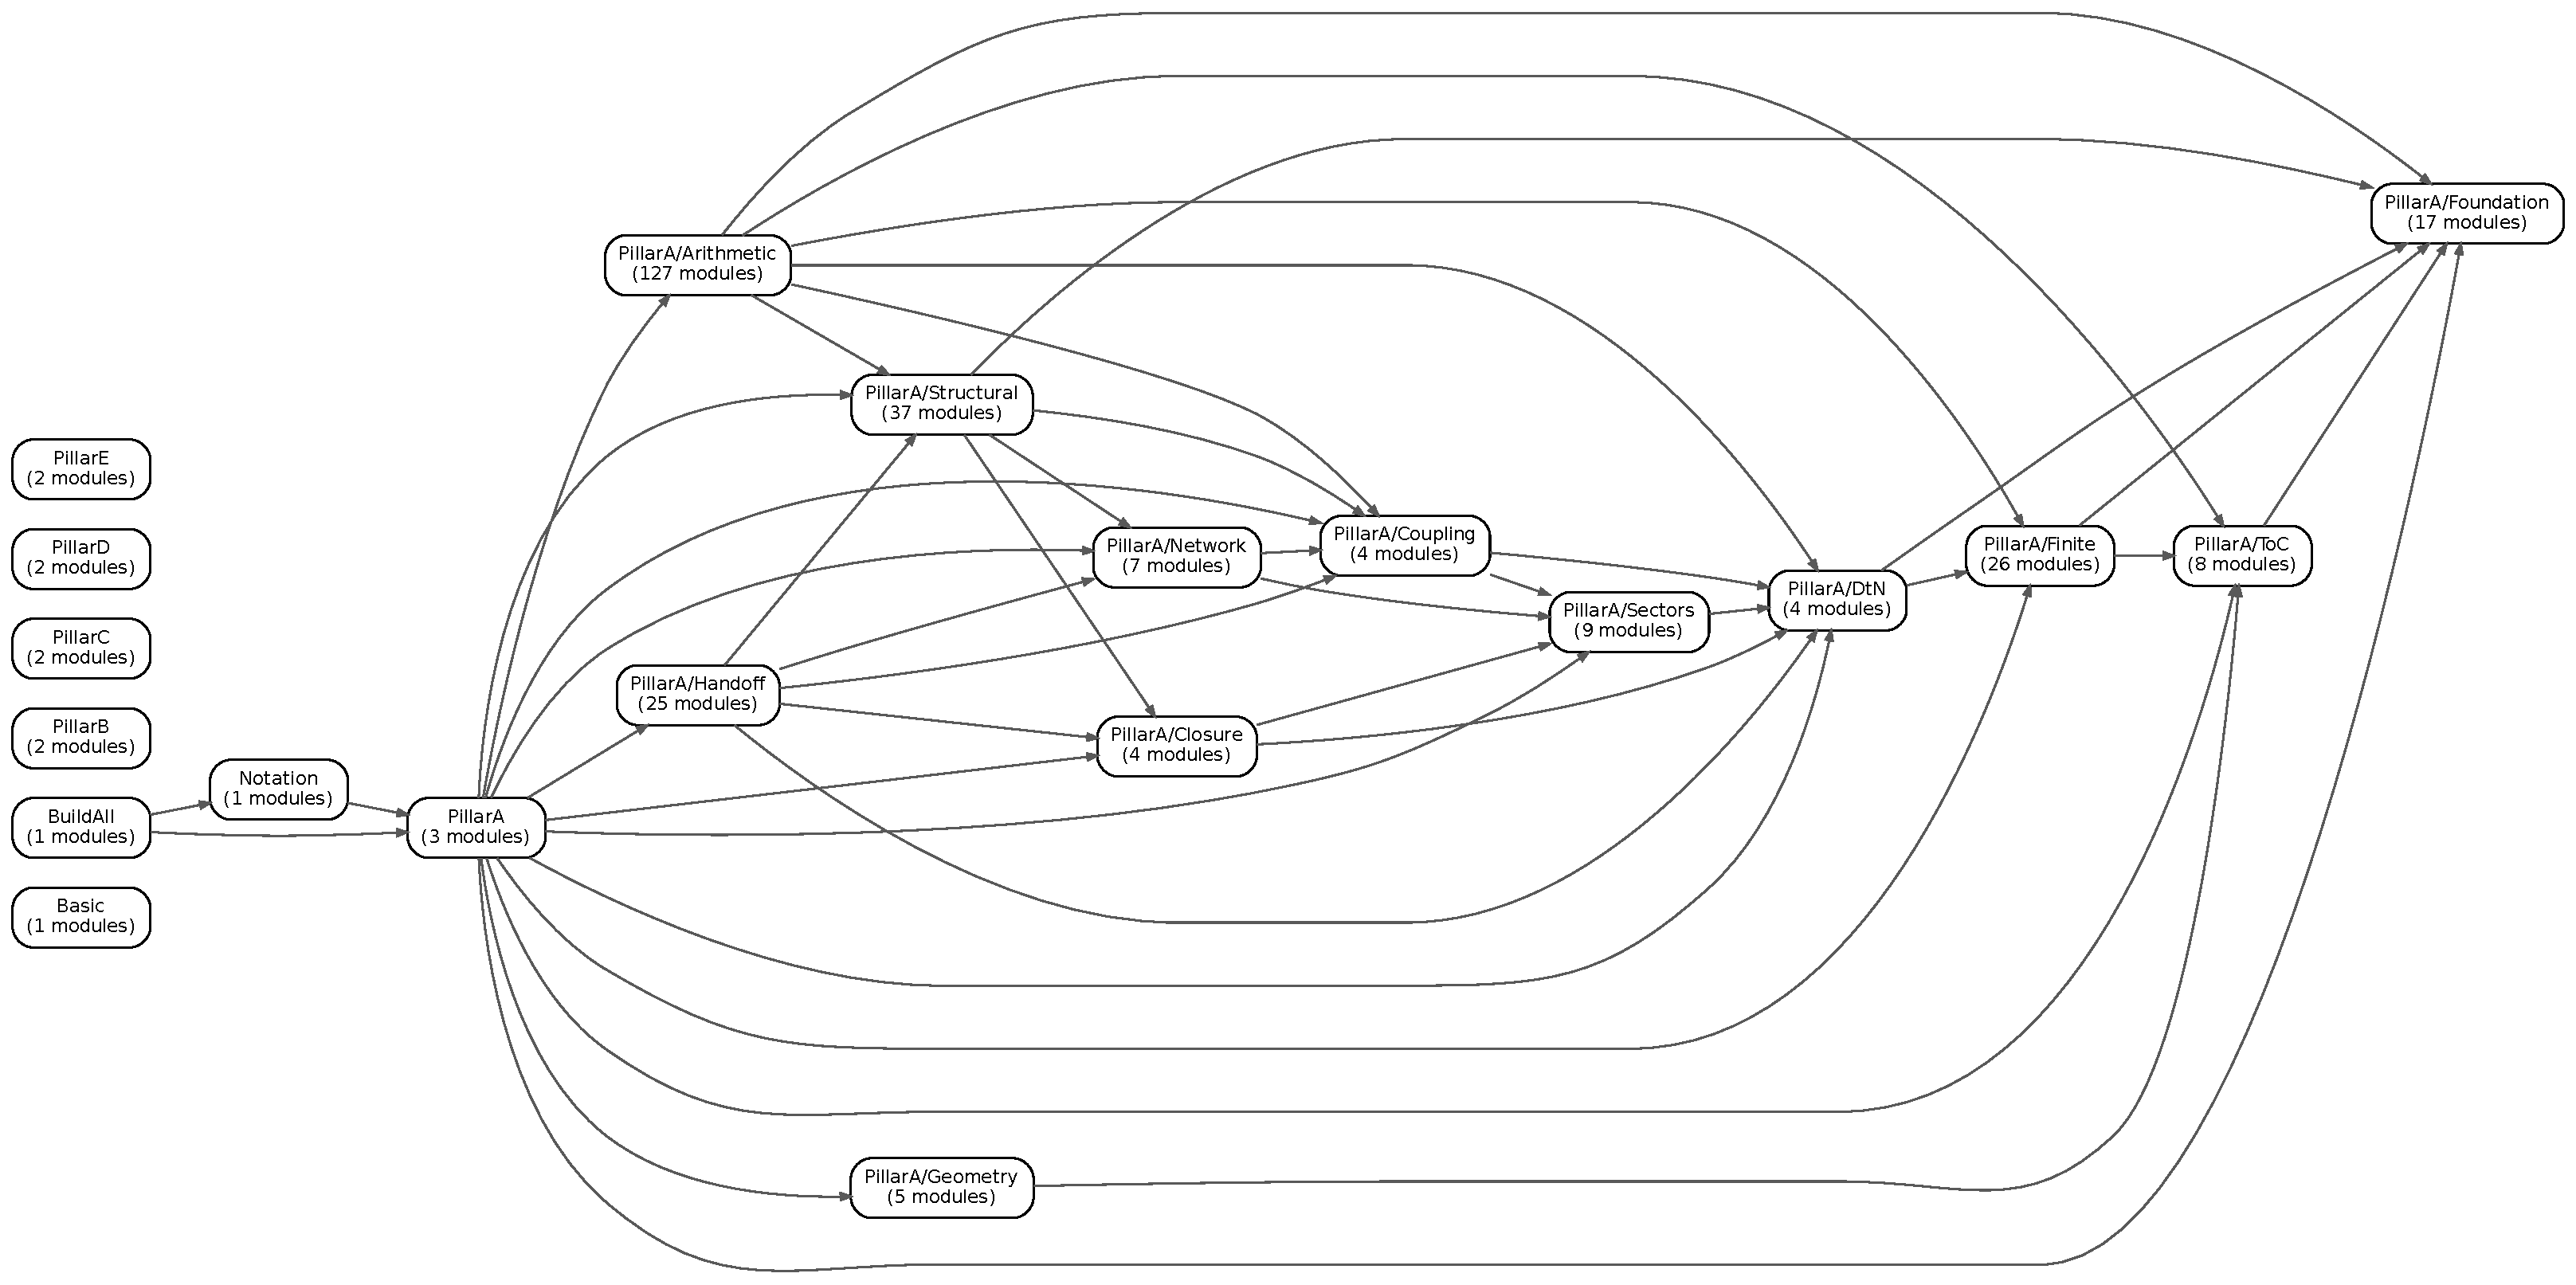
\includegraphics[width=0.98\linewidth,height=0.40\textheight,keepaspectratio]{figures/module_group_dependency_graph.pdf}\end{center}
\subsection*{Graph B: robust semantic core mainline}
\paragraph{Arrow convention.} An edge \(A \to B\) means that \(B\) is the next curated semantic construction step derived from \(A\) along the robust core mainline. The arrow points in the intended derived-only construction direction. This is a semantic mainline view, not a complete import graph.
\begin{center}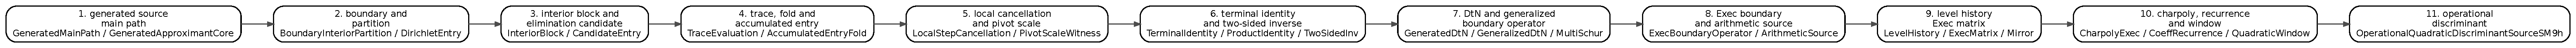
\includegraphics[width=0.98\linewidth,height=0.32\textheight,keepaspectratio]{figures/core_robust_semantic_mainline.pdf}\end{center}

\subsection*{Group summary}
\small
\arrayrulecolor{black!22}
\begin{longtable}{L{0.36\linewidth} L{0.1\linewidth} L{0.14\linewidth} L{0.14\linewidth} L{0.14\linewidth}}
\hline
\textbf{Group} & \textbf{Modules} & \textbf{Internal edges} & \textbf{Outgoing edges} & \textbf{Incoming edges}\\
\hline
\endfirsthead
\hline
\textbf{Group} & \textbf{Modules} & \textbf{Internal edges} & \textbf{Outgoing edges} & \textbf{Incoming edges}\\
\hline
\endhead
Basic & 1 & 0 & 0 & 0\\
\hline
\addlinespace[0.24em]
BuildAll & 1 & 0 & 2 & 0\\
\hline
\addlinespace[0.24em]
Notation & 1 & 0 & 1 & 1\\
\hline
\addlinespace[0.24em]
PillarA & 3 & 2 & 23 & 2\\
\hline
\addlinespace[0.24em]
PillarA/\allowbreak{}Arithmetic & 127 & 348 & 16 & 2\\
\hline
\addlinespace[0.24em]
PillarA/\allowbreak{}Closure & 4 & 5 & 2 & 5\\
\hline
\addlinespace[0.24em]
PillarA/\allowbreak{}Coupling & 4 & 5 & 2 & 6\\
\hline
\addlinespace[0.24em]
PillarA/\allowbreak{}DtN & 4 & 5 & 3 & 8\\
\hline
\addlinespace[0.24em]
PillarA/\allowbreak{}Finite & 26 & 58 & 4 & 4\\
\hline
\addlinespace[0.24em]
PillarA/\allowbreak{}Foundation & 17 & 45 & 0 & 25\\
\hline
\addlinespace[0.24em]
PillarA/\allowbreak{}Geometry & 5 & 7 & 1 & 2\\
\hline
\addlinespace[0.24em]
PillarA/\allowbreak{}Handoff & 25 & 46 & 7 & 2\\
\hline
\addlinespace[0.24em]
PillarA/\allowbreak{}Network & 7 & 13 & 2 & 4\\
\hline
\addlinespace[0.24em]
PillarA/\allowbreak{}Sectors & 9 & 15 & 1 & 5\\
\hline
\addlinespace[0.24em]
PillarA/\allowbreak{}Structural & 37 & 79 & 5 & 5\\
\hline
\addlinespace[0.24em]
PillarA/\allowbreak{}ToC & 8 & 15 & 8 & 6\\
\hline
\addlinespace[0.24em]
PillarB & 2 & 1 & 0 & 0\\
\hline
\addlinespace[0.24em]
PillarC & 2 & 1 & 0 & 0\\
\hline
\addlinespace[0.24em]
PillarD & 2 & 1 & 0 & 0\\
\hline
\addlinespace[0.24em]
PillarE & 2 & 1 & 0 & 0\\
\hline
\addlinespace[0.24em]
\end{longtable}
\arrayrulecolor{black}
\normalsize

\subsection*{Import hotspots}
\footnotesize
\arrayrulecolor{black!22}
\begin{longtable}{L{0.42\linewidth} L{0.16\linewidth} L{0.07\linewidth} L{0.08\linewidth} L{0.1\linewidth} L{0.09\linewidth}}
\hline
\textbf{Module} & \textbf{Group} & \textbf{Imports} & \textbf{Imported by} & \textbf{Transitive imports} & \textbf{Flags}\\
\hline
\endfirsthead
\hline
\textbf{Module} & \textbf{Group} & \textbf{Imports} & \textbf{Imported by} & \textbf{Transitive imports} & \textbf{Flags}\\
\hline
\endhead
\href{run:repo_snapshot/CNNA/PillarA/Arithmetic/BuildAll.lean}{CNNA.\allowbreak{}PillarA.\allowbreak{}Arithmetic.\allowbreak{}BuildAll} & PillarA/\allowbreak{}Arithmetic & 126 & 1 & 204 & BuildAll\\
\hline
\addlinespace[0.24em]
\href{run:repo_snapshot/CNNA/PillarA/Arithmetic/Notation.lean}{CNNA.\allowbreak{}PillarA.\allowbreak{}Arithmetic.\allowbreak{}Notation} & PillarA/\allowbreak{}Arithmetic & 80 & 2 & 175 & Notation\\
\hline
\addlinespace[0.24em]
\href{run:repo_snapshot/CNNA/PillarA/Structural/CayleyDickson/BuildAll.lean}{CNNA.\allowbreak{}PillarA.\allowbreak{}Structural.\allowbreak{}CayleyDickson.\allowbreak{}BuildAll} & PillarA/\allowbreak{}Structural & 35 & 1 & 75 & BuildAll\\
\hline
\addlinespace[0.24em]
\href{run:repo_snapshot/CNNA/PillarA/Finite/BuildAll.lean}{CNNA.\allowbreak{}PillarA.\allowbreak{}Finite.\allowbreak{}BuildAll} & PillarA/\allowbreak{}Finite & 17 & 1 & 46 & BuildAll\\
\hline
\addlinespace[0.24em]
\href{run:repo_snapshot/CNNA/PillarA/Foundation/BuildAll.lean}{CNNA.\allowbreak{}PillarA.\allowbreak{}Foundation.\allowbreak{}BuildAll} & PillarA/\allowbreak{}Foundation & 16 & 1 & 16 & BuildAll\\
\hline
\addlinespace[0.24em]
\href{run:repo_snapshot/CNNA/PillarA/BuildAll.lean}{CNNA.\allowbreak{}PillarA.\allowbreak{}BuildAll} & PillarA & 13 & 2 & 274 & BuildAll\\
\hline
\addlinespace[0.24em]
\href{run:repo_snapshot/CNNA/PillarA/Finite/Notation.lean}{CNNA.\allowbreak{}PillarA.\allowbreak{}Finite.\allowbreak{}Notation} & PillarA/\allowbreak{}Finite & 12 & 2 & 45 & Notation\\
\hline
\addlinespace[0.24em]
\href{run:repo_snapshot/CNNA/PillarA/Notation.lean}{CNNA.\allowbreak{}PillarA.\allowbreak{}Notation} & PillarA & 11 & 2 & 225 & Notation\\
\hline
\addlinespace[0.24em]
\href{run:repo_snapshot/CNNA/PillarA/Foundation/Notation.lean}{CNNA.\allowbreak{}PillarA.\allowbreak{}Foundation.\allowbreak{}Notation} & PillarA/\allowbreak{}Foundation & 10 & 4 & 13 & Notation\\
\hline
\addlinespace[0.24em]
\href{run:repo_snapshot/CNNA/PillarA/Handoff/BuildAll.lean}{CNNA.\allowbreak{}PillarA.\allowbreak{}Handoff.\allowbreak{}BuildAll} & PillarA/\allowbreak{}Handoff & 8 & 1 & 75 & BuildAll\\
\hline
\addlinespace[0.24em]
\href{run:repo_snapshot/CNNA/PillarA/Sectors/BuildAll.lean}{CNNA.\allowbreak{}PillarA.\allowbreak{}Sectors.\allowbreak{}BuildAll} & PillarA/\allowbreak{}Sectors & 8 & 1 & 35 & BuildAll\\
\hline
\addlinespace[0.24em]
\href{run:repo_snapshot/CNNA/PillarA/ToC/BuildAll.lean}{CNNA.\allowbreak{}PillarA.\allowbreak{}ToC.\allowbreak{}BuildAll} & PillarA/\allowbreak{}ToC & 7 & 2 & 21 & BuildAll\\
\hline
\addlinespace[0.24em]
\href{run:repo_snapshot/CNNA/PillarA/Finite/ExecSpectral/BuildAll.lean}{CNNA.\allowbreak{}PillarA.\allowbreak{}Finite.\allowbreak{}ExecSpectral.\allowbreak{}BuildAll} & PillarA/\allowbreak{}Finite & 6 & 2 & 32 & BuildAll\\
\hline
\addlinespace[0.24em]
\href{run:repo_snapshot/CNNA/PillarA/Handoff/Notation.lean}{CNNA.\allowbreak{}PillarA.\allowbreak{}Handoff.\allowbreak{}Notation} & PillarA/\allowbreak{}Handoff & 6 & 2 & 74 & Notation\\
\hline
\addlinespace[0.24em]
\href{run:repo_snapshot/CNNA/PillarA/Handoff/Outputs/BuildAll.lean}{CNNA.\allowbreak{}PillarA.\allowbreak{}Handoff.\allowbreak{}Outputs.\allowbreak{}BuildAll} & PillarA/\allowbreak{}Handoff & 6 & 2 & 61 & BuildAll\\
\hline
\addlinespace[0.24em]
\href{run:repo_snapshot/CNNA/PillarA/Network/BuildAll.lean}{CNNA.\allowbreak{}PillarA.\allowbreak{}Network.\allowbreak{}BuildAll} & PillarA/\allowbreak{}Network & 6 & 1 & 37 & BuildAll\\
\hline
\addlinespace[0.24em]
\href{run:repo_snapshot/CNNA/PillarA/Handoff/Core/SectorExport.lean}{CNNA.\allowbreak{}PillarA.\allowbreak{}Handoff.\allowbreak{}Core.\allowbreak{}SectorExport} & PillarA/\allowbreak{}Handoff & 5 & 5 & 42 & \\
\hline
\addlinespace[0.24em]
\href{run:repo_snapshot/CNNA/PillarA/Foundation/Interfaces.lean}{CNNA.\allowbreak{}PillarA.\allowbreak{}Foundation.\allowbreak{}Interfaces} & PillarA/\allowbreak{}Foundation & 4 & 3 & 6 & \\
\hline
\addlinespace[0.24em]
\href{run:repo_snapshot/CNNA/PillarA/Geometry/BuildAll.lean}{CNNA.\allowbreak{}PillarA.\allowbreak{}Geometry.\allowbreak{}BuildAll} & PillarA/\allowbreak{}Geometry & 4 & 1 & 20 & BuildAll\\
\hline
\addlinespace[0.24em]
\href{run:repo_snapshot/CNNA/PillarA/Handoff/Inputs/BuildAll.lean}{CNNA.\allowbreak{}PillarA.\allowbreak{}Handoff.\allowbreak{}Inputs.\allowbreak{}BuildAll} & PillarA/\allowbreak{}Handoff & 4 & 2 & 51 & BuildAll\\
\hline
\addlinespace[0.24em]
\end{longtable}
\arrayrulecolor{black}
\normalsize

\subsection*{Complete Lean module catalog, dependency-first order}
\footnotesize
\arrayrulecolor{black!22}
\begin{longtable}{L{0.025\linewidth} L{0.315\linewidth} L{0.08\linewidth} L{0.315\linewidth} L{0.045\linewidth} L{0.055\linewidth} L{0.07\linewidth}}
\hline
\textbf{\#} & \textbf{Module} & \textbf{Group} & \textbf{Path} & \textbf{Imports} & \textbf{Imported by} & \textbf{Flags}\\
\hline
\endfirsthead
\hline
\textbf{\#} & \textbf{Module} & \textbf{Group} & \textbf{Path} & \textbf{Imports} & \textbf{Imported by} & \textbf{Flags}\\
\hline
\endhead
1 & \href{run:repo_snapshot/CNNA/Basic.lean}{CNNA.\allowbreak{}Basic} & Basic & \href{run:repo_snapshot/CNNA/Basic.lean}{CNNA/\allowbreak{}Basic.\allowbreak{}lean} & 0 & 0 & ---\\
\hline
\addlinespace[0.24em]
2 & \href{run:repo_snapshot/CNNA/PillarA/Foundation/HermitianStructure.lean}{CNNA.\allowbreak{}PillarA.\allowbreak{}Foundation.\allowbreak{}HermitianStructure} & PillarA/\allowbreak{}Foundation & \href{run:repo_snapshot/CNNA/PillarA/Foundation/HermitianStructure.lean}{CNNA/\allowbreak{}PillarA/\allowbreak{}Foundation/\allowbreak{}HermitianStructure.\allowbreak{}lean} & 0 & 3 & ---\\
\hline
\addlinespace[0.24em]
3 & \href{run:repo_snapshot/CNNA/PillarA/Foundation/SubstrateClass.lean}{CNNA.\allowbreak{}PillarA.\allowbreak{}Foundation.\allowbreak{}SubstrateClass} & PillarA/\allowbreak{}Foundation & \href{run:repo_snapshot/CNNA/PillarA/Foundation/SubstrateClass.lean}{CNNA/\allowbreak{}PillarA/\allowbreak{}Foundation/\allowbreak{}SubstrateClass.\allowbreak{}lean} & 0 & 3 & ---\\
\hline
\addlinespace[0.24em]
4 & \href{run:repo_snapshot/CNNA/PillarB/BuildAll.lean}{CNNA.\allowbreak{}PillarB.\allowbreak{}BuildAll} & PillarB & \href{run:repo_snapshot/CNNA/PillarB/BuildAll.lean}{CNNA/\allowbreak{}PillarB/\allowbreak{}BuildAll.\allowbreak{}lean} & 0 & 1 & BuildAll\\
\hline
\addlinespace[0.24em]
5 & \href{run:repo_snapshot/CNNA/PillarC/BuildAll.lean}{CNNA.\allowbreak{}PillarC.\allowbreak{}BuildAll} & PillarC & \href{run:repo_snapshot/CNNA/PillarC/BuildAll.lean}{CNNA/\allowbreak{}PillarC/\allowbreak{}BuildAll.\allowbreak{}lean} & 0 & 1 & BuildAll\\
\hline
\addlinespace[0.24em]
6 & \href{run:repo_snapshot/CNNA/PillarD/BuildAll.lean}{CNNA.\allowbreak{}PillarD.\allowbreak{}BuildAll} & PillarD & \href{run:repo_snapshot/CNNA/PillarD/BuildAll.lean}{CNNA/\allowbreak{}PillarD/\allowbreak{}BuildAll.\allowbreak{}lean} & 0 & 1 & BuildAll\\
\hline
\addlinespace[0.24em]
7 & \href{run:repo_snapshot/CNNA/PillarE/BuildAll.lean}{CNNA.\allowbreak{}PillarE.\allowbreak{}BuildAll} & PillarE & \href{run:repo_snapshot/CNNA/PillarE/BuildAll.lean}{CNNA/\allowbreak{}PillarE/\allowbreak{}BuildAll.\allowbreak{}lean} & 0 & 1 & BuildAll\\
\hline
\addlinespace[0.24em]
8 & \href{run:repo_snapshot/CNNA/PillarA/Foundation/ExecComplex.lean}{CNNA.\allowbreak{}PillarA.\allowbreak{}Foundation.\allowbreak{}ExecComplex} & PillarA/\allowbreak{}Foundation & \href{run:repo_snapshot/CNNA/PillarA/Foundation/ExecComplex.lean}{CNNA/\allowbreak{}PillarA/\allowbreak{}Foundation/\allowbreak{}ExecComplex.\allowbreak{}lean} & 1 & 5 & ---\\
\hline
\addlinespace[0.24em]
9 & \href{run:repo_snapshot/CNNA/PillarA/Foundation/FiniteHilbert.lean}{CNNA.\allowbreak{}PillarA.\allowbreak{}Foundation.\allowbreak{}FiniteHilbert} & PillarA/\allowbreak{}Foundation & \href{run:repo_snapshot/CNNA/PillarA/Foundation/FiniteHilbert.lean}{CNNA/\allowbreak{}PillarA/\allowbreak{}Foundation/\allowbreak{}FiniteHilbert.\allowbreak{}lean} & 1 & 3 & ---\\
\hline
\addlinespace[0.24em]
10 & \href{run:repo_snapshot/CNNA/PillarB.lean}{CNNA.\allowbreak{}PillarB} & PillarB & \href{run:repo_snapshot/CNNA/PillarB.lean}{CNNA/\allowbreak{}PillarB.\allowbreak{}lean} & 1 & 0 & ---\\
\hline
\addlinespace[0.24em]
11 & \href{run:repo_snapshot/CNNA/PillarC.lean}{CNNA.\allowbreak{}PillarC} & PillarC & \href{run:repo_snapshot/CNNA/PillarC.lean}{CNNA/\allowbreak{}PillarC.\allowbreak{}lean} & 1 & 0 & ---\\
\hline
\addlinespace[0.24em]
12 & \href{run:repo_snapshot/CNNA/PillarD.lean}{CNNA.\allowbreak{}PillarD} & PillarD & \href{run:repo_snapshot/CNNA/PillarD.lean}{CNNA/\allowbreak{}PillarD.\allowbreak{}lean} & 1 & 0 & ---\\
\hline
\addlinespace[0.24em]
13 & \href{run:repo_snapshot/CNNA/PillarE.lean}{CNNA.\allowbreak{}PillarE} & PillarE & \href{run:repo_snapshot/CNNA/PillarE.lean}{CNNA/\allowbreak{}PillarE.\allowbreak{}lean} & 1 & 0 & ---\\
\hline
\addlinespace[0.24em]
14 & \href{run:repo_snapshot/CNNA/PillarA/Foundation/ExecComplexLemmas.lean}{CNNA.\allowbreak{}PillarA.\allowbreak{}Foundation.\allowbreak{}ExecComplexLemmas} & PillarA/\allowbreak{}Foundation & \href{run:repo_snapshot/CNNA/PillarA/Foundation/ExecComplexLemmas.lean}{CNNA/\allowbreak{}PillarA/\allowbreak{}Foundation/\allowbreak{}ExecComplexLemmas.\allowbreak{}lean} & 1 & 1 & ---\\
\hline
\addlinespace[0.24em]
15 & \href{run:repo_snapshot/CNNA/PillarA/Foundation/MatrixNorms.lean}{CNNA.\allowbreak{}PillarA.\allowbreak{}Foundation.\allowbreak{}MatrixNorms} & PillarA/\allowbreak{}Foundation & \href{run:repo_snapshot/CNNA/PillarA/Foundation/MatrixNorms.lean}{CNNA/\allowbreak{}PillarA/\allowbreak{}Foundation/\allowbreak{}MatrixNorms.\allowbreak{}lean} & 1 & 9 & ---\\
\hline
\addlinespace[0.24em]
16 & \href{run:repo_snapshot/CNNA/PillarA/Foundation/MatrixAlgebra.lean}{CNNA.\allowbreak{}PillarA.\allowbreak{}Foundation.\allowbreak{}MatrixAlgebra} & PillarA/\allowbreak{}Foundation & \href{run:repo_snapshot/CNNA/PillarA/Foundation/MatrixAlgebra.lean}{CNNA/\allowbreak{}PillarA/\allowbreak{}Foundation/\allowbreak{}MatrixAlgebra.\allowbreak{}lean} & 1 & 4 & ---\\
\hline
\addlinespace[0.24em]
17 & \href{run:repo_snapshot/CNNA/PillarA/Foundation/ExecComplexBridge.lean}{CNNA.\allowbreak{}PillarA.\allowbreak{}Foundation.\allowbreak{}ExecComplexBridge} & PillarA/\allowbreak{}Foundation & \href{run:repo_snapshot/CNNA/PillarA/Foundation/ExecComplexBridge.lean}{CNNA/\allowbreak{}PillarA/\allowbreak{}Foundation/\allowbreak{}ExecComplexBridge.\allowbreak{}lean} & 2 & 8 & ---\\
\hline
\addlinespace[0.24em]
18 & \href{run:repo_snapshot/CNNA/PillarA/Foundation/Interfaces.lean}{CNNA.\allowbreak{}PillarA.\allowbreak{}Foundation.\allowbreak{}Interfaces} & PillarA/\allowbreak{}Foundation & \href{run:repo_snapshot/CNNA/PillarA/Foundation/Interfaces.lean}{CNNA/\allowbreak{}PillarA/\allowbreak{}Foundation/\allowbreak{}Interfaces.\allowbreak{}lean} & 4 & 3 & ---\\
\hline
\addlinespace[0.24em]
19 & \href{run:repo_snapshot/CNNA/PillarA/Foundation/Determinism.lean}{CNNA.\allowbreak{}PillarA.\allowbreak{}Foundation.\allowbreak{}Determinism} & PillarA/\allowbreak{}Foundation & \href{run:repo_snapshot/CNNA/PillarA/Foundation/Determinism.lean}{CNNA/\allowbreak{}PillarA/\allowbreak{}Foundation/\allowbreak{}Determinism.\allowbreak{}lean} & 1 & 7 & ---\\
\hline
\addlinespace[0.24em]
20 & \href{run:repo_snapshot/CNNA/PillarA/Foundation/ConcreteSubstrate.lean}{CNNA.\allowbreak{}PillarA.\allowbreak{}Foundation.\allowbreak{}ConcreteSubstrate} & PillarA/\allowbreak{}Foundation & \href{run:repo_snapshot/CNNA/PillarA/Foundation/ConcreteSubstrate.lean}{CNNA/\allowbreak{}PillarA/\allowbreak{}Foundation/\allowbreak{}ConcreteSubstrate.\allowbreak{}lean} & 1 & 5 & ---\\
\hline
\addlinespace[0.24em]
21 & \href{run:repo_snapshot/CNNA/PillarA/Foundation/LevelVariableSubstrate.lean}{CNNA.\allowbreak{}PillarA.\allowbreak{}Foundation.\allowbreak{}LevelVariableSubstrate} & PillarA/\allowbreak{}Foundation & \href{run:repo_snapshot/CNNA/PillarA/Foundation/LevelVariableSubstrate.lean}{CNNA/\allowbreak{}PillarA/\allowbreak{}Foundation/\allowbreak{}LevelVariableSubstrate.\allowbreak{}lean} & 1 & 5 & ---\\
\hline
\addlinespace[0.24em]
22 & \href{run:repo_snapshot/CNNA/PillarA/Foundation/RegularizationPolicy.lean}{CNNA.\allowbreak{}PillarA.\allowbreak{}Foundation.\allowbreak{}RegularizationPolicy} & PillarA/\allowbreak{}Foundation & \href{run:repo_snapshot/CNNA/PillarA/Foundation/RegularizationPolicy.lean}{CNNA/\allowbreak{}PillarA/\allowbreak{}Foundation/\allowbreak{}RegularizationPolicy.\allowbreak{}lean} & 2 & 3 & ---\\
\hline
\addlinespace[0.24em]
23 & \href{run:repo_snapshot/CNNA/PillarA/Foundation/WeightPolicy.lean}{CNNA.\allowbreak{}PillarA.\allowbreak{}Foundation.\allowbreak{}WeightPolicy} & PillarA/\allowbreak{}Foundation & \href{run:repo_snapshot/CNNA/PillarA/Foundation/WeightPolicy.lean}{CNNA/\allowbreak{}PillarA/\allowbreak{}Foundation/\allowbreak{}WeightPolicy.\allowbreak{}lean} & 1 & 4 & ---\\
\hline
\addlinespace[0.24em]
24 & \href{run:repo_snapshot/CNNA/PillarA/Foundation/SubstrateAnalysis.lean}{CNNA.\allowbreak{}PillarA.\allowbreak{}Foundation.\allowbreak{}SubstrateAnalysis} & PillarA/\allowbreak{}Foundation & \href{run:repo_snapshot/CNNA/PillarA/Foundation/SubstrateAnalysis.lean}{CNNA/\allowbreak{}PillarA/\allowbreak{}Foundation/\allowbreak{}SubstrateAnalysis.\allowbreak{}lean} & 2 & 2 & ---\\
\hline
\addlinespace[0.24em]
25 & \href{run:repo_snapshot/CNNA/PillarA/Foundation/Notation.lean}{CNNA.\allowbreak{}PillarA.\allowbreak{}Foundation.\allowbreak{}Notation} & PillarA/\allowbreak{}Foundation & \href{run:repo_snapshot/CNNA/PillarA/Foundation/Notation.lean}{CNNA/\allowbreak{}PillarA/\allowbreak{}Foundation/\allowbreak{}Notation.\allowbreak{}lean} & 10 & 4 & Notation\\
\hline
\addlinespace[0.24em]
26 & \href{run:repo_snapshot/CNNA/PillarA/Foundation/BuildAll.lean}{CNNA.\allowbreak{}PillarA.\allowbreak{}Foundation.\allowbreak{}BuildAll} & PillarA/\allowbreak{}Foundation & \href{run:repo_snapshot/CNNA/PillarA/Foundation/BuildAll.lean}{CNNA/\allowbreak{}PillarA/\allowbreak{}Foundation/\allowbreak{}BuildAll.\allowbreak{}lean} & 16 & 1 & BuildAll\\
\hline
\addlinespace[0.24em]
27 & \href{run:repo_snapshot/CNNA/PillarA/ToC/Contract.lean}{CNNA.\allowbreak{}PillarA.\allowbreak{}ToC.\allowbreak{}Contract} & PillarA/\allowbreak{}ToC & \href{run:repo_snapshot/CNNA/PillarA/ToC/Contract.lean}{CNNA/\allowbreak{}PillarA/\allowbreak{}ToC/\allowbreak{}Contract.\allowbreak{}lean} & 2 & 2 & ---\\
\hline
\addlinespace[0.24em]
28 & \href{run:repo_snapshot/CNNA/PillarA/ToC/Addressing.lean}{CNNA.\allowbreak{}PillarA.\allowbreak{}ToC.\allowbreak{}Addressing} & PillarA/\allowbreak{}ToC & \href{run:repo_snapshot/CNNA/PillarA/ToC/Addressing.lean}{CNNA/\allowbreak{}PillarA/\allowbreak{}ToC/\allowbreak{}Addressing.\allowbreak{}lean} & 2 & 3 & ---\\
\hline
\addlinespace[0.24em]
29 & \href{run:repo_snapshot/CNNA/PillarA/Geometry/LCPMeasure.lean}{CNNA.\allowbreak{}PillarA.\allowbreak{}Geometry.\allowbreak{}LCPMeasure} & PillarA/\allowbreak{}Geometry & \href{run:repo_snapshot/CNNA/PillarA/Geometry/LCPMeasure.lean}{CNNA/\allowbreak{}PillarA/\allowbreak{}Geometry/\allowbreak{}LCPMeasure.\allowbreak{}lean} & 1 & 2 & ---\\
\hline
\addlinespace[0.24em]
30 & \href{run:repo_snapshot/CNNA/PillarA/ToC/IdealAddressEquiv.lean}{CNNA.\allowbreak{}PillarA.\allowbreak{}ToC.\allowbreak{}IdealAddressEquiv} & PillarA/\allowbreak{}ToC & \href{run:repo_snapshot/CNNA/PillarA/ToC/IdealAddressEquiv.lean}{CNNA/\allowbreak{}PillarA/\allowbreak{}ToC/\allowbreak{}IdealAddressEquiv.\allowbreak{}lean} & 1 & 3 & ---\\
\hline
\addlinespace[0.24em]
31 & \href{run:repo_snapshot/CNNA/PillarA/Geometry/Foliation.lean}{CNNA.\allowbreak{}PillarA.\allowbreak{}Geometry.\allowbreak{}Foliation} & PillarA/\allowbreak{}Geometry & \href{run:repo_snapshot/CNNA/PillarA/Geometry/Foliation.lean}{CNNA/\allowbreak{}PillarA/\allowbreak{}Geometry/\allowbreak{}Foliation.\allowbreak{}lean} & 1 & 2 & ---\\
\hline
\addlinespace[0.24em]
32 & \href{run:repo_snapshot/CNNA/PillarA/ToC/ConcreteIdeal.lean}{CNNA.\allowbreak{}PillarA.\allowbreak{}ToC.\allowbreak{}ConcreteIdeal} & PillarA/\allowbreak{}ToC & \href{run:repo_snapshot/CNNA/PillarA/ToC/ConcreteIdeal.lean}{CNNA/\allowbreak{}PillarA/\allowbreak{}ToC/\allowbreak{}ConcreteIdeal.\allowbreak{}lean} & 2 & 3 & ---\\
\hline
\addlinespace[0.24em]
33 & \href{run:repo_snapshot/CNNA/PillarA/Geometry/SpacetimePaths.lean}{CNNA.\allowbreak{}PillarA.\allowbreak{}Geometry.\allowbreak{}SpacetimePaths} & PillarA/\allowbreak{}Geometry & \href{run:repo_snapshot/CNNA/PillarA/Geometry/SpacetimePaths.lean}{CNNA/\allowbreak{}PillarA/\allowbreak{}Geometry/\allowbreak{}SpacetimePaths.\allowbreak{}lean} & 1 & 2 & ---\\
\hline
\addlinespace[0.24em]
34 & \href{run:repo_snapshot/CNNA/PillarA/ToC/Concrete.lean}{CNNA.\allowbreak{}PillarA.\allowbreak{}ToC.\allowbreak{}Concrete} & PillarA/\allowbreak{}ToC & \href{run:repo_snapshot/CNNA/PillarA/ToC/Concrete.lean}{CNNA/\allowbreak{}PillarA/\allowbreak{}ToC/\allowbreak{}Concrete.\allowbreak{}lean} & 4 & 3 & ---\\
\hline
\addlinespace[0.24em]
35 & \href{run:repo_snapshot/CNNA/PillarA/Geometry/Notation.lean}{CNNA.\allowbreak{}PillarA.\allowbreak{}Geometry.\allowbreak{}Notation} & PillarA/\allowbreak{}Geometry & \href{run:repo_snapshot/CNNA/PillarA/Geometry/Notation.lean}{CNNA/\allowbreak{}PillarA/\allowbreak{}Geometry/\allowbreak{}Notation.\allowbreak{}lean} & 1 & 2 & Notation\\
\hline
\addlinespace[0.24em]
36 & \href{run:repo_snapshot/CNNA/PillarA/ToC/GeneratedBranchFamily.lean}{CNNA.\allowbreak{}PillarA.\allowbreak{}ToC.\allowbreak{}GeneratedBranchFamily} & PillarA/\allowbreak{}ToC & \href{run:repo_snapshot/CNNA/PillarA/ToC/GeneratedBranchFamily.lean}{CNNA/\allowbreak{}PillarA/\allowbreak{}ToC/\allowbreak{}GeneratedBranchFamily.\allowbreak{}lean} & 3 & 2 & ---\\
\hline
\addlinespace[0.24em]
37 & \href{run:repo_snapshot/CNNA/PillarA/ToC/Notation.lean}{CNNA.\allowbreak{}PillarA.\allowbreak{}ToC.\allowbreak{}Notation} & PillarA/\allowbreak{}ToC & \href{run:repo_snapshot/CNNA/PillarA/ToC/Notation.lean}{CNNA/\allowbreak{}PillarA/\allowbreak{}ToC/\allowbreak{}Notation.\allowbreak{}lean} & 2 & 3 & Notation\\
\hline
\addlinespace[0.24em]
38 & \href{run:repo_snapshot/CNNA/PillarA/Geometry/BuildAll.lean}{CNNA.\allowbreak{}PillarA.\allowbreak{}Geometry.\allowbreak{}BuildAll} & PillarA/\allowbreak{}Geometry & \href{run:repo_snapshot/CNNA/PillarA/Geometry/BuildAll.lean}{CNNA/\allowbreak{}PillarA/\allowbreak{}Geometry/\allowbreak{}BuildAll.\allowbreak{}lean} & 4 & 1 & BuildAll\\
\hline
\addlinespace[0.24em]
39 & \href{run:repo_snapshot/CNNA/PillarA/Arithmetic/Smoke/GeneratedSource.lean}{CNNA.\allowbreak{}PillarA.\allowbreak{}Arithmetic.\allowbreak{}Smoke.\allowbreak{}GeneratedSource} & PillarA/\allowbreak{}Arithmetic & \href{run:repo_snapshot/CNNA/PillarA/Arithmetic/Smoke/GeneratedSource.lean}{CNNA/\allowbreak{}PillarA/\allowbreak{}Arithmetic/\allowbreak{}Smoke/\allowbreak{}GeneratedSource.\allowbreak{}lean} & 1 & 3 & ---\\
\hline
\addlinespace[0.24em]
40 & \href{run:repo_snapshot/CNNA/PillarA/Finite/CutSpec.lean}{CNNA.\allowbreak{}PillarA.\allowbreak{}Finite.\allowbreak{}CutSpec} & PillarA/\allowbreak{}Finite & \href{run:repo_snapshot/CNNA/PillarA/Finite/CutSpec.lean}{CNNA/\allowbreak{}PillarA/\allowbreak{}Finite/\allowbreak{}CutSpec.\allowbreak{}lean} & 1 & 2 & ---\\
\hline
\addlinespace[0.24em]
41 & \href{run:repo_snapshot/CNNA/PillarA/ToC/BuildAll.lean}{CNNA.\allowbreak{}PillarA.\allowbreak{}ToC.\allowbreak{}BuildAll} & PillarA/\allowbreak{}ToC & \href{run:repo_snapshot/CNNA/PillarA/ToC/BuildAll.lean}{CNNA/\allowbreak{}PillarA/\allowbreak{}ToC/\allowbreak{}BuildAll.\allowbreak{}lean} & 7 & 2 & BuildAll\\
\hline
\addlinespace[0.24em]
42 & \href{run:repo_snapshot/CNNA/PillarA/Arithmetic/Smoke/GeneratedMainPath.lean}{CNNA.\allowbreak{}PillarA.\allowbreak{}Arithmetic.\allowbreak{}Smoke.\allowbreak{}GeneratedMainPath} & PillarA/\allowbreak{}Arithmetic & \href{run:repo_snapshot/CNNA/PillarA/Arithmetic/Smoke/GeneratedMainPath.lean}{CNNA/\allowbreak{}PillarA/\allowbreak{}Arithmetic/\allowbreak{}Smoke/\allowbreak{}GeneratedMainPath.\allowbreak{}lean} & 1 & 3 & ---\\
\hline
\addlinespace[0.24em]
43 & \href{run:repo_snapshot/CNNA/PillarA/Finite/RegionCore.lean}{CNNA.\allowbreak{}PillarA.\allowbreak{}Finite.\allowbreak{}RegionCore} & PillarA/\allowbreak{}Finite & \href{run:repo_snapshot/CNNA/PillarA/Finite/RegionCore.lean}{CNNA/\allowbreak{}PillarA/\allowbreak{}Finite/\allowbreak{}RegionCore.\allowbreak{}lean} & 1 & 2 & ---\\
\hline
\addlinespace[0.24em]
44 & \href{run:repo_snapshot/CNNA/PillarA/Arithmetic/Smoke/GeneratedApproximantCore.lean}{CNNA.\allowbreak{}PillarA.\allowbreak{}Arithmetic.\allowbreak{}Smoke.\allowbreak{}GeneratedApproximantCore} & PillarA/\allowbreak{}Arithmetic & \href{run:repo_snapshot/CNNA/PillarA/Arithmetic/Smoke/GeneratedApproximantCore.lean}{CNNA/\allowbreak{}PillarA/\allowbreak{}Arithmetic/\allowbreak{}Smoke/\allowbreak{}GeneratedApproximantCore.\allowbreak{}lean} & 1 & 3 & ---\\
\hline
\addlinespace[0.24em]
45 & \href{run:repo_snapshot/CNNA/PillarA/Finite/BoundaryPorts.lean}{CNNA.\allowbreak{}PillarA.\allowbreak{}Finite.\allowbreak{}BoundaryPorts} & PillarA/\allowbreak{}Finite & \href{run:repo_snapshot/CNNA/PillarA/Finite/BoundaryPorts.lean}{CNNA/\allowbreak{}PillarA/\allowbreak{}Finite/\allowbreak{}BoundaryPorts.\allowbreak{}lean} & 1 & 2 & ---\\
\hline
\addlinespace[0.24em]
46 & \href{run:repo_snapshot/CNNA/PillarA/Arithmetic/Smoke/GeneratedBoundaryInteriorPartition.lean}{CNNA.\allowbreak{}PillarA.\allowbreak{}Arithmetic.\allowbreak{}Smoke.\allowbreak{}GeneratedBoundaryInteriorPartition} & PillarA/\allowbreak{}Arithmetic & \href{run:repo_snapshot/CNNA/PillarA/Arithmetic/Smoke/GeneratedBoundaryInteriorPartition.lean}{CNNA/\allowbreak{}PillarA/\allowbreak{}Arithmetic/\allowbreak{}Smoke/\allowbreak{}GeneratedBoundaryInteriorPartition.\allowbreak{}lean} & 1 & 3 & ---\\
\hline
\addlinespace[0.24em]
47 & \href{run:repo_snapshot/CNNA/PillarA/Finite/Approximant.lean}{CNNA.\allowbreak{}PillarA.\allowbreak{}Finite.\allowbreak{}Approximant} & PillarA/\allowbreak{}Finite & \href{run:repo_snapshot/CNNA/PillarA/Finite/Approximant.lean}{CNNA/\allowbreak{}PillarA/\allowbreak{}Finite/\allowbreak{}Approximant.\allowbreak{}lean} & 1 & 3 & ---\\
\hline
\addlinespace[0.24em]
48 & \href{run:repo_snapshot/CNNA/PillarA/Arithmetic/Smoke/GeneratedDirichletEntry.lean}{CNNA.\allowbreak{}PillarA.\allowbreak{}Arithmetic.\allowbreak{}Smoke.\allowbreak{}GeneratedDirichletEntry} & PillarA/\allowbreak{}Arithmetic & \href{run:repo_snapshot/CNNA/PillarA/Arithmetic/Smoke/GeneratedDirichletEntry.lean}{CNNA/\allowbreak{}PillarA/\allowbreak{}Arithmetic/\allowbreak{}Smoke/\allowbreak{}GeneratedDirichletEntry.\allowbreak{}lean} & 2 & 4 & ---\\
\hline
\addlinespace[0.24em]
49 & \href{run:repo_snapshot/CNNA/PillarA/Finite/DirichletLaplacian.lean}{CNNA.\allowbreak{}PillarA.\allowbreak{}Finite.\allowbreak{}DirichletLaplacian} & PillarA/\allowbreak{}Finite & \href{run:repo_snapshot/CNNA/PillarA/Finite/DirichletLaplacian.lean}{CNNA/\allowbreak{}PillarA/\allowbreak{}Finite/\allowbreak{}DirichletLaplacian.\allowbreak{}lean} & 3 & 4 & ---\\
\hline
\addlinespace[0.24em]
50 & \href{run:repo_snapshot/CNNA/PillarA/Finite/Selection.lean}{CNNA.\allowbreak{}PillarA.\allowbreak{}Finite.\allowbreak{}Selection} & PillarA/\allowbreak{}Finite & \href{run:repo_snapshot/CNNA/PillarA/Finite/Selection.lean}{CNNA/\allowbreak{}PillarA/\allowbreak{}Finite/\allowbreak{}Selection.\allowbreak{}lean} & 1 & 2 & ---\\
\hline
\addlinespace[0.24em]
51 & \href{run:repo_snapshot/CNNA/PillarA/Arithmetic/Smoke/GeneratedDirichletExecEntrySourceSM3bq.lean}{CNNA.\allowbreak{}PillarA.\allowbreak{}Arithmetic.\allowbreak{}Smoke.\allowbreak{}GeneratedDirichletExecEntrySourceSM3bq} & PillarA/\allowbreak{}Arithmetic & \href{run:repo_snapshot/CNNA/PillarA/Arithmetic/Smoke/GeneratedDirichletExecEntrySourceSM3bq.lean}{CNNA/\allowbreak{}PillarA/\allowbreak{}Arithmetic/\allowbreak{}Smoke/\allowbreak{}GeneratedDirichletExecEntrySourceSM3bq.\allowbreak{}lean} & 2 & 2 & ---\\
\hline
\addlinespace[0.24em]
52 & \href{run:repo_snapshot/CNNA/PillarA/Arithmetic/Smoke/GeneratedInteriorBlock.lean}{CNNA.\allowbreak{}PillarA.\allowbreak{}Arithmetic.\allowbreak{}Smoke.\allowbreak{}GeneratedInteriorBlock} & PillarA/\allowbreak{}Arithmetic & \href{run:repo_snapshot/CNNA/PillarA/Arithmetic/Smoke/GeneratedInteriorBlock.lean}{CNNA/\allowbreak{}PillarA/\allowbreak{}Arithmetic/\allowbreak{}Smoke/\allowbreak{}GeneratedInteriorBlock.\allowbreak{}lean} & 1 & 3 & ---\\
\hline
\addlinespace[0.24em]
53 & \href{run:repo_snapshot/CNNA/PillarA/DtN/DtN.lean}{CNNA.\allowbreak{}PillarA.\allowbreak{}DtN.\allowbreak{}DtN} & PillarA/\allowbreak{}DtN & \href{run:repo_snapshot/CNNA/PillarA/DtN/DtN.lean}{CNNA/\allowbreak{}PillarA/\allowbreak{}DtN/\allowbreak{}DtN.\allowbreak{}lean} & 1 & 5 & ---\\
\hline
\addlinespace[0.24em]
54 & \href{run:repo_snapshot/CNNA/PillarA/Finite/SpectralDecompositionCore.lean}{CNNA.\allowbreak{}PillarA.\allowbreak{}Finite.\allowbreak{}SpectralDecompositionCore} & PillarA/\allowbreak{}Finite & \href{run:repo_snapshot/CNNA/PillarA/Finite/SpectralDecompositionCore.lean}{CNNA/\allowbreak{}PillarA/\allowbreak{}Finite/\allowbreak{}SpectralDecompositionCore.\allowbreak{}lean} & 1 & 3 & ---\\
\hline
\addlinespace[0.24em]
55 & \href{run:repo_snapshot/CNNA/PillarA/Arithmetic/Smoke/GeneratedInteriorEliminationCandidate.lean}{CNNA.\allowbreak{}PillarA.\allowbreak{}Arithmetic.\allowbreak{}Smoke.\allowbreak{}GeneratedInteriorEliminationCandidate} & PillarA/\allowbreak{}Arithmetic & \href{run:repo_snapshot/CNNA/PillarA/Arithmetic/Smoke/GeneratedInteriorEliminationCandidate.lean}{CNNA/\allowbreak{}PillarA/\allowbreak{}Arithmetic/\allowbreak{}Smoke/\allowbreak{}GeneratedInteriorEliminationCandidate.\allowbreak{}lean} & 1 & 3 & ---\\
\hline
\addlinespace[0.24em]
56 & \href{run:repo_snapshot/CNNA/PillarA/DtN/DtNStabilized.lean}{CNNA.\allowbreak{}PillarA.\allowbreak{}DtN.\allowbreak{}DtNStabilized} & PillarA/\allowbreak{}DtN & \href{run:repo_snapshot/CNNA/PillarA/DtN/DtNStabilized.lean}{CNNA/\allowbreak{}PillarA/\allowbreak{}DtN/\allowbreak{}DtNStabilized.\allowbreak{}lean} & 3 & 4 & ---\\
\hline
\addlinespace[0.24em]
57 & \href{run:repo_snapshot/CNNA/PillarA/Finite/ExecSpectral/PolynomialCore.lean}{CNNA.\allowbreak{}PillarA.\allowbreak{}Finite.\allowbreak{}ExecSpectral.\allowbreak{}PolynomialCore} & PillarA/\allowbreak{}Finite & \href{run:repo_snapshot/CNNA/PillarA/Finite/ExecSpectral/PolynomialCore.lean}{CNNA/\allowbreak{}PillarA/\allowbreak{}Finite/\allowbreak{}ExecSpectral/\allowbreak{}PolynomialCore.\allowbreak{}lean} & 1 & 2 & ---\\
\hline
\addlinespace[0.24em]
58 & \href{run:repo_snapshot/CNNA/PillarA/Finite/SpectralDecompositionC.lean}{CNNA.\allowbreak{}PillarA.\allowbreak{}Finite.\allowbreak{}SpectralDecompositionC} & PillarA/\allowbreak{}Finite & \href{run:repo_snapshot/CNNA/PillarA/Finite/SpectralDecompositionC.lean}{CNNA/\allowbreak{}PillarA/\allowbreak{}Finite/\allowbreak{}SpectralDecompositionC.\allowbreak{}lean} & 2 & 3 & ---\\
\hline
\addlinespace[0.24em]
59 & \href{run:repo_snapshot/CNNA/PillarA/Arithmetic/Smoke/GeneratedInteriorEliminationCandidateEntry.lean}{CNNA.\allowbreak{}PillarA.\allowbreak{}Arithmetic.\allowbreak{}Smoke.\allowbreak{}GeneratedInteriorEliminationCandidateEntry} & PillarA/\allowbreak{}Arithmetic & \href{run:repo_snapshot/CNNA/PillarA/Arithmetic/Smoke/GeneratedInteriorEliminationCandidateEntry.lean}{CNNA/\allowbreak{}PillarA/\allowbreak{}Arithmetic/\allowbreak{}Smoke/\allowbreak{}GeneratedInteriorEliminationCandidateEntry.\allowbreak{}lean} & 1 & 3 & ---\\
\hline
\addlinespace[0.24em]
60 & \href{run:repo_snapshot/CNNA/PillarA/DtN/Notation.lean}{CNNA.\allowbreak{}PillarA.\allowbreak{}DtN.\allowbreak{}Notation} & PillarA/\allowbreak{}DtN & \href{run:repo_snapshot/CNNA/PillarA/DtN/Notation.lean}{CNNA/\allowbreak{}PillarA/\allowbreak{}DtN/\allowbreak{}Notation.\allowbreak{}lean} & 1 & 3 & Notation\\
\hline
\addlinespace[0.24em]
61 & \href{run:repo_snapshot/CNNA/PillarA/Sectors/BranchPatch.lean}{CNNA.\allowbreak{}PillarA.\allowbreak{}Sectors.\allowbreak{}BranchPatch} & PillarA/\allowbreak{}Sectors & \href{run:repo_snapshot/CNNA/PillarA/Sectors/BranchPatch.lean}{CNNA/\allowbreak{}PillarA/\allowbreak{}Sectors/\allowbreak{}BranchPatch.\allowbreak{}lean} & 1 & 2 & ---\\
\hline
\addlinespace[0.24em]
62 & \href{run:repo_snapshot/CNNA/PillarA/Finite/ExecSpectral/CharpolyCore.lean}{CNNA.\allowbreak{}PillarA.\allowbreak{}Finite.\allowbreak{}ExecSpectral.\allowbreak{}CharpolyCore} & PillarA/\allowbreak{}Finite & \href{run:repo_snapshot/CNNA/PillarA/Finite/ExecSpectral/CharpolyCore.lean}{CNNA/\allowbreak{}PillarA/\allowbreak{}Finite/\allowbreak{}ExecSpectral/\allowbreak{}CharpolyCore.\allowbreak{}lean} & 1 & 2 & ---\\
\hline
\addlinespace[0.24em]
63 & \href{run:repo_snapshot/CNNA/PillarA/Finite/SpectralBridge.lean}{CNNA.\allowbreak{}PillarA.\allowbreak{}Finite.\allowbreak{}SpectralBridge} & PillarA/\allowbreak{}Finite & \href{run:repo_snapshot/CNNA/PillarA/Finite/SpectralBridge.lean}{CNNA/\allowbreak{}PillarA/\allowbreak{}Finite/\allowbreak{}SpectralBridge.\allowbreak{}lean} & 1 & 3 & ---\\
\hline
\addlinespace[0.24em]
64 & \href{run:repo_snapshot/CNNA/PillarA/Arithmetic/Smoke/GeneratedInteriorTwoSidedInv.lean}{CNNA.\allowbreak{}PillarA.\allowbreak{}Arithmetic.\allowbreak{}Smoke.\allowbreak{}GeneratedInteriorTwoSidedInv} & PillarA/\allowbreak{}Arithmetic & \href{run:repo_snapshot/CNNA/PillarA/Arithmetic/Smoke/GeneratedInteriorTwoSidedInv.lean}{CNNA/\allowbreak{}PillarA/\allowbreak{}Arithmetic/\allowbreak{}Smoke/\allowbreak{}GeneratedInteriorTwoSidedInv.\allowbreak{}lean} & 2 & 3 & ---\\
\hline
\addlinespace[0.24em]
65 & \href{run:repo_snapshot/CNNA/PillarA/DtN/BuildAll.lean}{CNNA.\allowbreak{}PillarA.\allowbreak{}DtN.\allowbreak{}BuildAll} & PillarA/\allowbreak{}DtN & \href{run:repo_snapshot/CNNA/PillarA/DtN/BuildAll.lean}{CNNA/\allowbreak{}PillarA/\allowbreak{}DtN/\allowbreak{}BuildAll.\allowbreak{}lean} & 3 & 1 & BuildAll\\
\hline
\addlinespace[0.24em]
66 & \href{run:repo_snapshot/CNNA/PillarA/Sectors/ComplementSectorFamily.lean}{CNNA.\allowbreak{}PillarA.\allowbreak{}Sectors.\allowbreak{}ComplementSectorFamily} & PillarA/\allowbreak{}Sectors & \href{run:repo_snapshot/CNNA/PillarA/Sectors/ComplementSectorFamily.lean}{CNNA/\allowbreak{}PillarA/\allowbreak{}Sectors/\allowbreak{}ComplementSectorFamily.\allowbreak{}lean} & 1 & 2 & ---\\
\hline
\addlinespace[0.24em]
67 & \href{run:repo_snapshot/CNNA/PillarA/Finite/ExecSpectral/RootIsolation.lean}{CNNA.\allowbreak{}PillarA.\allowbreak{}Finite.\allowbreak{}ExecSpectral.\allowbreak{}RootIsolation} & PillarA/\allowbreak{}Finite & \href{run:repo_snapshot/CNNA/PillarA/Finite/ExecSpectral/RootIsolation.lean}{CNNA/\allowbreak{}PillarA/\allowbreak{}Finite/\allowbreak{}ExecSpectral/\allowbreak{}RootIsolation.\allowbreak{}lean} & 1 & 2 & ---\\
\hline
\addlinespace[0.24em]
68 & \href{run:repo_snapshot/CNNA/PillarA/Finite/StateSpace.lean}{CNNA.\allowbreak{}PillarA.\allowbreak{}Finite.\allowbreak{}StateSpace} & PillarA/\allowbreak{}Finite & \href{run:repo_snapshot/CNNA/PillarA/Finite/StateSpace.lean}{CNNA/\allowbreak{}PillarA/\allowbreak{}Finite/\allowbreak{}StateSpace.\allowbreak{}lean} & 1 & 3 & ---\\
\hline
\addlinespace[0.24em]
69 & \href{run:repo_snapshot/CNNA/PillarA/Arithmetic/Smoke/GeneratedInteriorInverseCandidateStart.lean}{CNNA.\allowbreak{}PillarA.\allowbreak{}Arithmetic.\allowbreak{}Smoke.\allowbreak{}GeneratedInteriorInverseCandidateStart} & PillarA/\allowbreak{}Arithmetic & \href{run:repo_snapshot/CNNA/PillarA/Arithmetic/Smoke/GeneratedInteriorInverseCandidateStart.lean}{CNNA/\allowbreak{}PillarA/\allowbreak{}Arithmetic/\allowbreak{}Smoke/\allowbreak{}GeneratedInteriorInverseCandidateStart.\allowbreak{}lean} & 1 & 3 & ---\\
\hline
\addlinespace[0.24em]
70 & \href{run:repo_snapshot/CNNA/PillarA/Sectors/SectorSplit.lean}{CNNA.\allowbreak{}PillarA.\allowbreak{}Sectors.\allowbreak{}SectorSplit} & PillarA/\allowbreak{}Sectors & \href{run:repo_snapshot/CNNA/PillarA/Sectors/SectorSplit.lean}{CNNA/\allowbreak{}PillarA/\allowbreak{}Sectors/\allowbreak{}SectorSplit.\allowbreak{}lean} & 1 & 4 & ---\\
\hline
\addlinespace[0.24em]
71 & \href{run:repo_snapshot/CNNA/PillarA/Finite/ExecSpectral/EigenvectorKernel.lean}{CNNA.\allowbreak{}PillarA.\allowbreak{}Finite.\allowbreak{}ExecSpectral.\allowbreak{}EigenvectorKernel} & PillarA/\allowbreak{}Finite & \href{run:repo_snapshot/CNNA/PillarA/Finite/ExecSpectral/EigenvectorKernel.lean}{CNNA/\allowbreak{}PillarA/\allowbreak{}Finite/\allowbreak{}ExecSpectral/\allowbreak{}EigenvectorKernel.\allowbreak{}lean} & 1 & 2 & ---\\
\hline
\addlinespace[0.24em]
72 & \href{run:repo_snapshot/CNNA/PillarA/Finite/MatrixExponential.lean}{CNNA.\allowbreak{}PillarA.\allowbreak{}Finite.\allowbreak{}MatrixExponential} & PillarA/\allowbreak{}Finite & \href{run:repo_snapshot/CNNA/PillarA/Finite/MatrixExponential.lean}{CNNA/\allowbreak{}PillarA/\allowbreak{}Finite/\allowbreak{}MatrixExponential.\allowbreak{}lean} & 1 & 4 & ---\\
\hline
\addlinespace[0.24em]
73 & \href{run:repo_snapshot/CNNA/PillarA/Arithmetic/Smoke/GeneratedInteriorEliminationCarrier.lean}{CNNA.\allowbreak{}PillarA.\allowbreak{}Arithmetic.\allowbreak{}Smoke.\allowbreak{}GeneratedInteriorEliminationCarrier} & PillarA/\allowbreak{}Arithmetic & \href{run:repo_snapshot/CNNA/PillarA/Arithmetic/Smoke/GeneratedInteriorEliminationCarrier.lean}{CNNA/\allowbreak{}PillarA/\allowbreak{}Arithmetic/\allowbreak{}Smoke/\allowbreak{}GeneratedInteriorEliminationCarrier.\allowbreak{}lean} & 1 & 3 & ---\\
\hline
\addlinespace[0.24em]
74 & \href{run:repo_snapshot/CNNA/PillarA/Coupling/GeneralizedDtN.lean}{CNNA.\allowbreak{}PillarA.\allowbreak{}Coupling.\allowbreak{}GeneralizedDtN} & PillarA/\allowbreak{}Coupling & \href{run:repo_snapshot/CNNA/PillarA/Coupling/GeneralizedDtN.lean}{CNNA/\allowbreak{}PillarA/\allowbreak{}Coupling/\allowbreak{}GeneralizedDtN.\allowbreak{}lean} & 2 & 3 & ---\\
\hline
\addlinespace[0.24em]
75 & \href{run:repo_snapshot/CNNA/PillarA/Network/RegionNet.lean}{CNNA.\allowbreak{}PillarA.\allowbreak{}Network.\allowbreak{}RegionNet} & PillarA/\allowbreak{}Network & \href{run:repo_snapshot/CNNA/PillarA/Network/RegionNet.lean}{CNNA/\allowbreak{}PillarA/\allowbreak{}Network/\allowbreak{}RegionNet.\allowbreak{}lean} & 1 & 3 & ---\\
\hline
\addlinespace[0.24em]
76 & \href{run:repo_snapshot/CNNA/PillarA/Sectors/BranchingWitness.lean}{CNNA.\allowbreak{}PillarA.\allowbreak{}Sectors.\allowbreak{}BranchingWitness} & PillarA/\allowbreak{}Sectors & \href{run:repo_snapshot/CNNA/PillarA/Sectors/BranchingWitness.lean}{CNNA/\allowbreak{}PillarA/\allowbreak{}Sectors/\allowbreak{}BranchingWitness.\allowbreak{}lean} & 1 & 2 & ---\\
\hline
\addlinespace[0.24em]
77 & \href{run:repo_snapshot/CNNA/PillarA/Finite/ExecSpectral/ProjectorCore.lean}{CNNA.\allowbreak{}PillarA.\allowbreak{}Finite.\allowbreak{}ExecSpectral.\allowbreak{}ProjectorCore} & PillarA/\allowbreak{}Finite & \href{run:repo_snapshot/CNNA/PillarA/Finite/ExecSpectral/ProjectorCore.lean}{CNNA/\allowbreak{}PillarA/\allowbreak{}Finite/\allowbreak{}ExecSpectral/\allowbreak{}ProjectorCore.\allowbreak{}lean} & 1 & 2 & ---\\
\hline
\addlinespace[0.24em]
78 & \href{run:repo_snapshot/CNNA/PillarA/Finite/GibbsStateSeed.lean}{CNNA.\allowbreak{}PillarA.\allowbreak{}Finite.\allowbreak{}GibbsStateSeed} & PillarA/\allowbreak{}Finite & \href{run:repo_snapshot/CNNA/PillarA/Finite/GibbsStateSeed.lean}{CNNA/\allowbreak{}PillarA/\allowbreak{}Finite/\allowbreak{}GibbsStateSeed.\allowbreak{}lean} & 1 & 2 & ---\\
\hline
\addlinespace[0.24em]
79 & \href{run:repo_snapshot/CNNA/PillarA/Finite/UnitaryEvolution.lean}{CNNA.\allowbreak{}PillarA.\allowbreak{}Finite.\allowbreak{}UnitaryEvolution} & PillarA/\allowbreak{}Finite & \href{run:repo_snapshot/CNNA/PillarA/Finite/UnitaryEvolution.lean}{CNNA/\allowbreak{}PillarA/\allowbreak{}Finite/\allowbreak{}UnitaryEvolution.\allowbreak{}lean} & 1 & 3 & ---\\
\hline
\addlinespace[0.24em]
80 & \href{run:repo_snapshot/CNNA/PillarA/Arithmetic/Smoke/GeneratedInteriorEliminationStep.lean}{CNNA.\allowbreak{}PillarA.\allowbreak{}Arithmetic.\allowbreak{}Smoke.\allowbreak{}GeneratedInteriorEliminationStep} & PillarA/\allowbreak{}Arithmetic & \href{run:repo_snapshot/CNNA/PillarA/Arithmetic/Smoke/GeneratedInteriorEliminationStep.lean}{CNNA/\allowbreak{}PillarA/\allowbreak{}Arithmetic/\allowbreak{}Smoke/\allowbreak{}GeneratedInteriorEliminationStep.\allowbreak{}lean} & 1 & 3 & ---\\
\hline
\addlinespace[0.24em]
81 & \href{run:repo_snapshot/CNNA/PillarA/Coupling/MultiSchur.lean}{CNNA.\allowbreak{}PillarA.\allowbreak{}Coupling.\allowbreak{}MultiSchur} & PillarA/\allowbreak{}Coupling & \href{run:repo_snapshot/CNNA/PillarA/Coupling/MultiSchur.lean}{CNNA/\allowbreak{}PillarA/\allowbreak{}Coupling/\allowbreak{}MultiSchur.\allowbreak{}lean} & 1 & 5 & ---\\
\hline
\addlinespace[0.24em]
82 & \href{run:repo_snapshot/CNNA/PillarA/Network/SectorChannels.lean}{CNNA.\allowbreak{}PillarA.\allowbreak{}Network.\allowbreak{}SectorChannels} & PillarA/\allowbreak{}Network & \href{run:repo_snapshot/CNNA/PillarA/Network/SectorChannels.lean}{CNNA/\allowbreak{}PillarA/\allowbreak{}Network/\allowbreak{}SectorChannels.\allowbreak{}lean} & 1 & 3 & ---\\
\hline
\addlinespace[0.24em]
83 & \href{run:repo_snapshot/CNNA/PillarA/Network/InfiniteCarrier.lean}{CNNA.\allowbreak{}PillarA.\allowbreak{}Network.\allowbreak{}InfiniteCarrier} & PillarA/\allowbreak{}Network & \href{run:repo_snapshot/CNNA/PillarA/Network/InfiniteCarrier.lean}{CNNA/\allowbreak{}PillarA/\allowbreak{}Network/\allowbreak{}InfiniteCarrier.\allowbreak{}lean} & 1 & 4 & ---\\
\hline
\addlinespace[0.24em]
84 & \href{run:repo_snapshot/CNNA/PillarA/Sectors/SelectedBranching.lean}{CNNA.\allowbreak{}PillarA.\allowbreak{}Sectors.\allowbreak{}SelectedBranching} & PillarA/\allowbreak{}Sectors & \href{run:repo_snapshot/CNNA/PillarA/Sectors/SelectedBranching.lean}{CNNA/\allowbreak{}PillarA/\allowbreak{}Sectors/\allowbreak{}SelectedBranching.\allowbreak{}lean} & 1 & 2 & ---\\
\hline
\addlinespace[0.24em]
85 & \href{run:repo_snapshot/CNNA/PillarA/Finite/ExecSpectral/Certificates.lean}{CNNA.\allowbreak{}PillarA.\allowbreak{}Finite.\allowbreak{}ExecSpectral.\allowbreak{}Certificates} & PillarA/\allowbreak{}Finite & \href{run:repo_snapshot/CNNA/PillarA/Finite/ExecSpectral/Certificates.lean}{CNNA/\allowbreak{}PillarA/\allowbreak{}Finite/\allowbreak{}ExecSpectral/\allowbreak{}Certificates.\allowbreak{}lean} & 1 & 2 & ---\\
\hline
\addlinespace[0.24em]
86 & \href{run:repo_snapshot/CNNA/PillarA/Finite/DynamicsAdapter.lean}{CNNA.\allowbreak{}PillarA.\allowbreak{}Finite.\allowbreak{}DynamicsAdapter} & PillarA/\allowbreak{}Finite & \href{run:repo_snapshot/CNNA/PillarA/Finite/DynamicsAdapter.lean}{CNNA/\allowbreak{}PillarA/\allowbreak{}Finite/\allowbreak{}DynamicsAdapter.\allowbreak{}lean} & 1 & 3 & ---\\
\hline
\addlinespace[0.24em]
87 & \href{run:repo_snapshot/CNNA/PillarA/Arithmetic/Smoke/GeneratedInteriorEliminationTrace.lean}{CNNA.\allowbreak{}PillarA.\allowbreak{}Arithmetic.\allowbreak{}Smoke.\allowbreak{}GeneratedInteriorEliminationTrace} & PillarA/\allowbreak{}Arithmetic & \href{run:repo_snapshot/CNNA/PillarA/Arithmetic/Smoke/GeneratedInteriorEliminationTrace.lean}{CNNA/\allowbreak{}PillarA/\allowbreak{}Arithmetic/\allowbreak{}Smoke/\allowbreak{}GeneratedInteriorEliminationTrace.\allowbreak{}lean} & 1 & 3 & ---\\
\hline
\addlinespace[0.24em]
88 & \href{run:repo_snapshot/CNNA/PillarA/Coupling/Notation.lean}{CNNA.\allowbreak{}PillarA.\allowbreak{}Coupling.\allowbreak{}Notation} & PillarA/\allowbreak{}Coupling & \href{run:repo_snapshot/CNNA/PillarA/Coupling/Notation.lean}{CNNA/\allowbreak{}PillarA/\allowbreak{}Coupling/\allowbreak{}Notation.\allowbreak{}lean} & 1 & 2 & Notation\\
\hline
\addlinespace[0.24em]
89 & \href{run:repo_snapshot/CNNA/PillarA/Network/SectorSysEnv.lean}{CNNA.\allowbreak{}PillarA.\allowbreak{}Network.\allowbreak{}SectorSysEnv} & PillarA/\allowbreak{}Network & \href{run:repo_snapshot/CNNA/PillarA/Network/SectorSysEnv.lean}{CNNA/\allowbreak{}PillarA/\allowbreak{}Network/\allowbreak{}SectorSysEnv.\allowbreak{}lean} & 1 & 2 & ---\\
\hline
\addlinespace[0.24em]
90 & \href{run:repo_snapshot/CNNA/PillarA/Sectors/UVSpectralSelector.lean}{CNNA.\allowbreak{}PillarA.\allowbreak{}Sectors.\allowbreak{}UVSpectralSelector} & PillarA/\allowbreak{}Sectors & \href{run:repo_snapshot/CNNA/PillarA/Sectors/UVSpectralSelector.lean}{CNNA/\allowbreak{}PillarA/\allowbreak{}Sectors/\allowbreak{}UVSpectralSelector.\allowbreak{}lean} & 1 & 2 & ---\\
\hline
\addlinespace[0.24em]
91 & \href{run:repo_snapshot/CNNA/PillarA/Finite/ExecSpectral/BuildAll.lean}{CNNA.\allowbreak{}PillarA.\allowbreak{}Finite.\allowbreak{}ExecSpectral.\allowbreak{}BuildAll} & PillarA/\allowbreak{}Finite & \href{run:repo_snapshot/CNNA/PillarA/Finite/ExecSpectral/BuildAll.lean}{CNNA/\allowbreak{}PillarA/\allowbreak{}Finite/\allowbreak{}ExecSpectral/\allowbreak{}BuildAll.\allowbreak{}lean} & 6 & 2 & BuildAll\\
\hline
\addlinespace[0.24em]
92 & \href{run:repo_snapshot/CNNA/PillarA/Finite/SpectralDecomposition.lean}{CNNA.\allowbreak{}PillarA.\allowbreak{}Finite.\allowbreak{}SpectralDecomposition} & PillarA/\allowbreak{}Finite & \href{run:repo_snapshot/CNNA/PillarA/Finite/SpectralDecomposition.lean}{CNNA/\allowbreak{}PillarA/\allowbreak{}Finite/\allowbreak{}SpectralDecomposition.\allowbreak{}lean} & 2 & 2 & ---\\
\hline
\addlinespace[0.24em]
93 & \href{run:repo_snapshot/CNNA/PillarA/Finite/ChannelSeed.lean}{CNNA.\allowbreak{}PillarA.\allowbreak{}Finite.\allowbreak{}ChannelSeed} & PillarA/\allowbreak{}Finite & \href{run:repo_snapshot/CNNA/PillarA/Finite/ChannelSeed.lean}{CNNA/\allowbreak{}PillarA/\allowbreak{}Finite/\allowbreak{}ChannelSeed.\allowbreak{}lean} & 1 & 3 & ---\\
\hline
\addlinespace[0.24em]
94 & \href{run:repo_snapshot/CNNA/PillarA/Arithmetic/Smoke/GeneratedInteriorInverseCandidateEntry.lean}{CNNA.\allowbreak{}PillarA.\allowbreak{}Arithmetic.\allowbreak{}Smoke.\allowbreak{}GeneratedInteriorInverseCandidateEntry} & PillarA/\allowbreak{}Arithmetic & \href{run:repo_snapshot/CNNA/PillarA/Arithmetic/Smoke/GeneratedInteriorInverseCandidateEntry.lean}{CNNA/\allowbreak{}PillarA/\allowbreak{}Arithmetic/\allowbreak{}Smoke/\allowbreak{}GeneratedInteriorInverseCandidateEntry.\allowbreak{}lean} & 1 & 3 & ---\\
\hline
\addlinespace[0.24em]
95 & \href{run:repo_snapshot/CNNA/PillarA/Coupling/BuildAll.lean}{CNNA.\allowbreak{}PillarA.\allowbreak{}Coupling.\allowbreak{}BuildAll} & PillarA/\allowbreak{}Coupling & \href{run:repo_snapshot/CNNA/PillarA/Coupling/BuildAll.lean}{CNNA/\allowbreak{}PillarA/\allowbreak{}Coupling/\allowbreak{}BuildAll.\allowbreak{}lean} & 3 & 1 & BuildAll\\
\hline
\addlinespace[0.24em]
96 & \href{run:repo_snapshot/CNNA/PillarA/Network/RelativeEntropyFlow.lean}{CNNA.\allowbreak{}PillarA.\allowbreak{}Network.\allowbreak{}RelativeEntropyFlow} & PillarA/\allowbreak{}Network & \href{run:repo_snapshot/CNNA/PillarA/Network/RelativeEntropyFlow.lean}{CNNA/\allowbreak{}PillarA/\allowbreak{}Network/\allowbreak{}RelativeEntropyFlow.\allowbreak{}lean} & 1 & 2 & ---\\
\hline
\addlinespace[0.24em]
97 & \href{run:repo_snapshot/CNNA/PillarA/Sectors/BranchingSelector.lean}{CNNA.\allowbreak{}PillarA.\allowbreak{}Sectors.\allowbreak{}BranchingSelector} & PillarA/\allowbreak{}Sectors & \href{run:repo_snapshot/CNNA/PillarA/Sectors/BranchingSelector.lean}{CNNA/\allowbreak{}PillarA/\allowbreak{}Sectors/\allowbreak{}BranchingSelector.\allowbreak{}lean} & 1 & 3 & ---\\
\hline
\addlinespace[0.24em]
98 & \href{run:repo_snapshot/CNNA/PillarA/Finite/ExecSpectral/Notation.lean}{CNNA.\allowbreak{}PillarA.\allowbreak{}Finite.\allowbreak{}ExecSpectral.\allowbreak{}Notation} & PillarA/\allowbreak{}Finite & \href{run:repo_snapshot/CNNA/PillarA/Finite/ExecSpectral/Notation.lean}{CNNA/\allowbreak{}PillarA/\allowbreak{}Finite/\allowbreak{}ExecSpectral/\allowbreak{}Notation.\allowbreak{}lean} & 1 & 1 & Notation\\
\hline
\addlinespace[0.24em]
99 & \href{run:repo_snapshot/CNNA/PillarA/Arithmetic/Core/Source.lean}{CNNA.\allowbreak{}PillarA.\allowbreak{}Arithmetic.\allowbreak{}Core.\allowbreak{}Source} & PillarA/\allowbreak{}Arithmetic & \href{run:repo_snapshot/CNNA/PillarA/Arithmetic/Core/Source.lean}{CNNA/\allowbreak{}PillarA/\allowbreak{}Arithmetic/\allowbreak{}Core/\allowbreak{}Source.\allowbreak{}lean} & 3 & 4 & ---\\
\hline
\addlinespace[0.24em]
100 & \href{run:repo_snapshot/CNNA/PillarA/Arithmetic/Smoke/GeneratedInteriorAccumulatedTraceEvaluation.lean}{CNNA.\allowbreak{}PillarA.\allowbreak{}Arithmetic.\allowbreak{}Smoke.\allowbreak{}GeneratedInteriorAccumulatedTraceEvaluation} & PillarA/\allowbreak{}Arithmetic & \href{run:repo_snapshot/CNNA/PillarA/Arithmetic/Smoke/GeneratedInteriorAccumulatedTraceEvaluation.lean}{CNNA/\allowbreak{}PillarA/\allowbreak{}Arithmetic/\allowbreak{}Smoke/\allowbreak{}GeneratedInteriorAccumulatedTraceEvaluation.\allowbreak{}lean} & 1 & 4 & ---\\
\hline
\addlinespace[0.24em]
101 & \href{run:repo_snapshot/CNNA/PillarA/Network/Notation.lean}{CNNA.\allowbreak{}PillarA.\allowbreak{}Network.\allowbreak{}Notation} & PillarA/\allowbreak{}Network & \href{run:repo_snapshot/CNNA/PillarA/Network/Notation.lean}{CNNA/\allowbreak{}PillarA/\allowbreak{}Network/\allowbreak{}Notation.\allowbreak{}lean} & 4 & 2 & Notation\\
\hline
\addlinespace[0.24em]
102 & \href{run:repo_snapshot/CNNA/PillarA/Closure/ParameterClosure.lean}{CNNA.\allowbreak{}PillarA.\allowbreak{}Closure.\allowbreak{}ParameterClosure} & PillarA/\allowbreak{}Closure & \href{run:repo_snapshot/CNNA/PillarA/Closure/ParameterClosure.lean}{CNNA/\allowbreak{}PillarA/\allowbreak{}Closure/\allowbreak{}ParameterClosure.\allowbreak{}lean} & 2 & 2 & ---\\
\hline
\addlinespace[0.24em]
103 & \href{run:repo_snapshot/CNNA/PillarA/Sectors/Notation.lean}{CNNA.\allowbreak{}PillarA.\allowbreak{}Sectors.\allowbreak{}Notation} & PillarA/\allowbreak{}Sectors & \href{run:repo_snapshot/CNNA/PillarA/Sectors/Notation.lean}{CNNA/\allowbreak{}PillarA/\allowbreak{}Sectors/\allowbreak{}Notation.\allowbreak{}lean} & 1 & 2 & Notation\\
\hline
\addlinespace[0.24em]
104 & \href{run:repo_snapshot/CNNA/PillarA/Finite/Notation.lean}{CNNA.\allowbreak{}PillarA.\allowbreak{}Finite.\allowbreak{}Notation} & PillarA/\allowbreak{}Finite & \href{run:repo_snapshot/CNNA/PillarA/Finite/Notation.lean}{CNNA/\allowbreak{}PillarA/\allowbreak{}Finite/\allowbreak{}Notation.\allowbreak{}lean} & 12 & 2 & Notation\\
\hline
\addlinespace[0.24em]
105 & \href{run:repo_snapshot/CNNA/PillarA/Arithmetic/BoundarySource/LevelHistoryIndex.lean}{CNNA.\allowbreak{}PillarA.\allowbreak{}Arithmetic.\allowbreak{}BoundarySource.\allowbreak{}LevelHistoryIndex} & PillarA/\allowbreak{}Arithmetic & \href{run:repo_snapshot/CNNA/PillarA/Arithmetic/BoundarySource/LevelHistoryIndex.lean}{CNNA/\allowbreak{}PillarA/\allowbreak{}Arithmetic/\allowbreak{}BoundarySource/\allowbreak{}LevelHistoryIndex.\allowbreak{}lean} & 1 & 2 & ---\\
\hline
\addlinespace[0.24em]
106 & \href{run:repo_snapshot/CNNA/PillarA/Arithmetic/Core/FullBoundaryAudit.lean}{CNNA.\allowbreak{}PillarA.\allowbreak{}Arithmetic.\allowbreak{}Core.\allowbreak{}FullBoundaryAudit} & PillarA/\allowbreak{}Arithmetic & \href{run:repo_snapshot/CNNA/PillarA/Arithmetic/Core/FullBoundaryAudit.lean}{CNNA/\allowbreak{}PillarA/\allowbreak{}Arithmetic/\allowbreak{}Core/\allowbreak{}FullBoundaryAudit.\allowbreak{}lean} & 1 & 3 & ---\\
\hline
\addlinespace[0.24em]
107 & \href{run:repo_snapshot/CNNA/PillarA/Arithmetic/Smoke/GeneratedInteriorBlockFoldNormalFormR3c1a.lean}{CNNA.\allowbreak{}PillarA.\allowbreak{}Arithmetic.\allowbreak{}Smoke.\allowbreak{}GeneratedInteriorBlockFoldNormalFormR3c1a} & PillarA/\allowbreak{}Arithmetic & \href{run:repo_snapshot/CNNA/PillarA/Arithmetic/Smoke/GeneratedInteriorBlockFoldNormalFormR3c1a.lean}{CNNA/\allowbreak{}PillarA/\allowbreak{}Arithmetic/\allowbreak{}Smoke/\allowbreak{}GeneratedInteriorBlockFoldNormalFormR3c1a.\allowbreak{}lean} & 1 & 4 & ---\\
\hline
\addlinespace[0.24em]
108 & \href{run:repo_snapshot/CNNA/PillarA/Arithmetic/Smoke/GeneratedInteriorInverseCandidateMatrix.lean}{CNNA.\allowbreak{}PillarA.\allowbreak{}Arithmetic.\allowbreak{}Smoke.\allowbreak{}GeneratedInteriorInverseCandidateMatrix} & PillarA/\allowbreak{}Arithmetic & \href{run:repo_snapshot/CNNA/PillarA/Arithmetic/Smoke/GeneratedInteriorInverseCandidateMatrix.lean}{CNNA/\allowbreak{}PillarA/\allowbreak{}Arithmetic/\allowbreak{}Smoke/\allowbreak{}GeneratedInteriorInverseCandidateMatrix.\allowbreak{}lean} & 1 & 3 & ---\\
\hline
\addlinespace[0.24em]
109 & \href{run:repo_snapshot/CNNA/PillarA/Network/BuildAll.lean}{CNNA.\allowbreak{}PillarA.\allowbreak{}Network.\allowbreak{}BuildAll} & PillarA/\allowbreak{}Network & \href{run:repo_snapshot/CNNA/PillarA/Network/BuildAll.lean}{CNNA/\allowbreak{}PillarA/\allowbreak{}Network/\allowbreak{}BuildAll.\allowbreak{}lean} & 6 & 1 & BuildAll\\
\hline
\addlinespace[0.24em]
110 & \href{run:repo_snapshot/CNNA/PillarA/Closure/RegularizationClosure.lean}{CNNA.\allowbreak{}PillarA.\allowbreak{}Closure.\allowbreak{}RegularizationClosure} & PillarA/\allowbreak{}Closure & \href{run:repo_snapshot/CNNA/PillarA/Closure/RegularizationClosure.lean}{CNNA/\allowbreak{}PillarA/\allowbreak{}Closure/\allowbreak{}RegularizationClosure.\allowbreak{}lean} & 1 & 4 & ---\\
\hline
\addlinespace[0.24em]
111 & \href{run:repo_snapshot/CNNA/PillarA/Sectors/BuildAll.lean}{CNNA.\allowbreak{}PillarA.\allowbreak{}Sectors.\allowbreak{}BuildAll} & PillarA/\allowbreak{}Sectors & \href{run:repo_snapshot/CNNA/PillarA/Sectors/BuildAll.lean}{CNNA/\allowbreak{}PillarA/\allowbreak{}Sectors/\allowbreak{}BuildAll.\allowbreak{}lean} & 8 & 1 & BuildAll\\
\hline
\addlinespace[0.24em]
112 & \href{run:repo_snapshot/CNNA/PillarA/Finite/BuildAll.lean}{CNNA.\allowbreak{}PillarA.\allowbreak{}Finite.\allowbreak{}BuildAll} & PillarA/\allowbreak{}Finite & \href{run:repo_snapshot/CNNA/PillarA/Finite/BuildAll.lean}{CNNA/\allowbreak{}PillarA/\allowbreak{}Finite/\allowbreak{}BuildAll.\allowbreak{}lean} & 17 & 1 & BuildAll\\
\hline
\addlinespace[0.24em]
113 & \href{run:repo_snapshot/CNNA/PillarA/Arithmetic/BoundarySource/LevelStepWitness.lean}{CNNA.\allowbreak{}PillarA.\allowbreak{}Arithmetic.\allowbreak{}BoundarySource.\allowbreak{}LevelStepWitness} & PillarA/\allowbreak{}Arithmetic & \href{run:repo_snapshot/CNNA/PillarA/Arithmetic/BoundarySource/LevelStepWitness.lean}{CNNA/\allowbreak{}PillarA/\allowbreak{}Arithmetic/\allowbreak{}BoundarySource/\allowbreak{}LevelStepWitness.\allowbreak{}lean} & 1 & 2 & ---\\
\hline
\addlinespace[0.24em]
114 & \href{run:repo_snapshot/CNNA/PillarA/Arithmetic/BoundarySource/ExistingIdealThreadNoGo.lean}{CNNA.\allowbreak{}PillarA.\allowbreak{}Arithmetic.\allowbreak{}BoundarySource.\allowbreak{}ExistingIdealThreadNoGo} & PillarA/\allowbreak{}Arithmetic & \href{run:repo_snapshot/CNNA/PillarA/Arithmetic/BoundarySource/ExistingIdealThreadNoGo.lean}{CNNA/\allowbreak{}PillarA/\allowbreak{}Arithmetic/\allowbreak{}BoundarySource/\allowbreak{}ExistingIdealThreadNoGo.\allowbreak{}lean} & 1 & 2 & ---\\
\hline
\addlinespace[0.24em]
115 & \href{run:repo_snapshot/CNNA/PillarA/Arithmetic/Smoke/GeneratedInteriorAccumulatedEntryCancellationR3c1.lean}{CNNA.\allowbreak{}PillarA.\allowbreak{}Arithmetic.\allowbreak{}Smoke.\allowbreak{}GeneratedInteriorAccumulatedEntryCancellationR3c1} & PillarA/\allowbreak{}Arithmetic & \href{run:repo_snapshot/CNNA/PillarA/Arithmetic/Smoke/GeneratedInteriorAccumulatedEntryCancellationR3c1.lean}{CNNA/\allowbreak{}PillarA/\allowbreak{}Arithmetic/\allowbreak{}Smoke/\allowbreak{}GeneratedInteriorAccumulatedEntryCancellationR3c1.\allowbreak{}lean} & 1 & 3 & ---\\
\hline
\addlinespace[0.24em]
116 & \href{run:repo_snapshot/CNNA/PillarA/Arithmetic/Smoke/GeneratedInteriorLocalStepSchurCancellationSourceAuditR3c1b0.lean}{CNNA.\allowbreak{}PillarA.\allowbreak{}Arithmetic.\allowbreak{}Smoke.\allowbreak{}GeneratedInteriorLocalStepSchurCancellationSourceAuditR3c1b0} & PillarA/\allowbreak{}Arithmetic & \href{run:repo_snapshot/CNNA/PillarA/Arithmetic/Smoke/GeneratedInteriorLocalStepSchurCancellationSourceAuditR3c1b0.lean}{CNNA/\allowbreak{}PillarA/\allowbreak{}Arithmetic/\allowbreak{}Smoke/\allowbreak{}GeneratedInteriorLocalStepSchurCancellationSourceAuditR3c1b0.\allowbreak{}lean} & 1 & 3 & ---\\
\hline
\addlinespace[0.24em]
117 & \href{run:repo_snapshot/CNNA/PillarA/Arithmetic/Smoke/GeneratedInteriorInverseCandidateShapeSeparation.lean}{CNNA.\allowbreak{}PillarA.\allowbreak{}Arithmetic.\allowbreak{}Smoke.\allowbreak{}GeneratedInteriorInverseCandidateShapeSeparation} & PillarA/\allowbreak{}Arithmetic & \href{run:repo_snapshot/CNNA/PillarA/Arithmetic/Smoke/GeneratedInteriorInverseCandidateShapeSeparation.lean}{CNNA/\allowbreak{}PillarA/\allowbreak{}Arithmetic/\allowbreak{}Smoke/\allowbreak{}GeneratedInteriorInverseCandidateShapeSeparation.\allowbreak{}lean} & 1 & 3 & ---\\
\hline
\addlinespace[0.24em]
118 & \href{run:repo_snapshot/CNNA/PillarA/Closure/Notation.lean}{CNNA.\allowbreak{}PillarA.\allowbreak{}Closure.\allowbreak{}Notation} & PillarA/\allowbreak{}Closure & \href{run:repo_snapshot/CNNA/PillarA/Closure/Notation.lean}{CNNA/\allowbreak{}PillarA/\allowbreak{}Closure/\allowbreak{}Notation.\allowbreak{}lean} & 1 & 3 & Notation\\
\hline
\addlinespace[0.24em]
119 & \href{run:repo_snapshot/CNNA/PillarA/Structural/CayleyDickson/Source.lean}{CNNA.\allowbreak{}PillarA.\allowbreak{}Structural.\allowbreak{}CayleyDickson.\allowbreak{}Source} & PillarA/\allowbreak{}Structural & \href{run:repo_snapshot/CNNA/PillarA/Structural/CayleyDickson/Source.lean}{CNNA/\allowbreak{}PillarA/\allowbreak{}Structural/\allowbreak{}CayleyDickson/\allowbreak{}Source.\allowbreak{}lean} & 3 & 2 & ---\\
\hline
\addlinespace[0.24em]
120 & \href{run:repo_snapshot/CNNA/PillarA/Arithmetic/BoundarySource/RecursiveLevelHistoryCarrier.lean}{CNNA.\allowbreak{}PillarA.\allowbreak{}Arithmetic.\allowbreak{}BoundarySource.\allowbreak{}RecursiveLevelHistoryCarrier} & PillarA/\allowbreak{}Arithmetic & \href{run:repo_snapshot/CNNA/PillarA/Arithmetic/BoundarySource/RecursiveLevelHistoryCarrier.lean}{CNNA/\allowbreak{}PillarA/\allowbreak{}Arithmetic/\allowbreak{}BoundarySource/\allowbreak{}RecursiveLevelHistoryCarrier.\allowbreak{}lean} & 1 & 2 & ---\\
\hline
\addlinespace[0.24em]
121 & \href{run:repo_snapshot/CNNA/PillarA/Arithmetic/Smoke/GeneratedInteriorLocalStepSchurCancellationInvariantSM3db2aR.lean}{CNNA.\allowbreak{}PillarA.\allowbreak{}Arithmetic.\allowbreak{}Smoke.\allowbreak{}GeneratedInteriorLocalStepSchurCancellationInvariantSM3db2aR} & PillarA/\allowbreak{}Arithmetic & \href{run:repo_snapshot/CNNA/PillarA/Arithmetic/Smoke/GeneratedInteriorLocalStepSchurCancellationInvariantSM3db2aR.lean}{CNNA/\allowbreak{}PillarA/\allowbreak{}Arithmetic/\allowbreak{}Smoke/\allowbreak{}GeneratedInteriorLocalStepSchurCancellationInvariantSM3db2aR.\allowbreak{}lean} & 1 & 3 & ---\\
\hline
\addlinespace[0.24em]
122 & \href{run:repo_snapshot/CNNA/PillarA/Arithmetic/Smoke/SM3dbRToSM3eRHandoff.lean}{CNNA.\allowbreak{}PillarA.\allowbreak{}Arithmetic.\allowbreak{}Smoke.\allowbreak{}SM3dbRToSM3eRHandoff} & PillarA/\allowbreak{}Arithmetic & \href{run:repo_snapshot/CNNA/PillarA/Arithmetic/Smoke/SM3dbRToSM3eRHandoff.lean}{CNNA/\allowbreak{}PillarA/\allowbreak{}Arithmetic/\allowbreak{}Smoke/\allowbreak{}SM3dbRToSM3eRHandoff.\allowbreak{}lean} & 1 & 4 & ---\\
\hline
\addlinespace[0.24em]
123 & \href{run:repo_snapshot/CNNA/PillarA/Closure/BuildAll.lean}{CNNA.\allowbreak{}PillarA.\allowbreak{}Closure.\allowbreak{}BuildAll} & PillarA/\allowbreak{}Closure & \href{run:repo_snapshot/CNNA/PillarA/Closure/BuildAll.lean}{CNNA/\allowbreak{}PillarA/\allowbreak{}Closure/\allowbreak{}BuildAll.\allowbreak{}lean} & 3 & 1 & BuildAll\\
\hline
\addlinespace[0.24em]
124 & \href{run:repo_snapshot/CNNA/PillarA/Handoff/Core/SectorExport.lean}{CNNA.\allowbreak{}PillarA.\allowbreak{}Handoff.\allowbreak{}Core.\allowbreak{}SectorExport} & PillarA/\allowbreak{}Handoff & \href{run:repo_snapshot/CNNA/PillarA/Handoff/Core/SectorExport.lean}{CNNA/\allowbreak{}PillarA/\allowbreak{}Handoff/\allowbreak{}Core/\allowbreak{}SectorExport.\allowbreak{}lean} & 5 & 5 & ---\\
\hline
\addlinespace[0.24em]
125 & \href{run:repo_snapshot/CNNA/PillarA/Structural/CayleyDickson/S6AdditionalFinding.lean}{CNNA.\allowbreak{}PillarA.\allowbreak{}Structural.\allowbreak{}CayleyDickson.\allowbreak{}S6AdditionalFinding} & PillarA/\allowbreak{}Structural & \href{run:repo_snapshot/CNNA/PillarA/Structural/CayleyDickson/S6AdditionalFinding.lean}{CNNA/\allowbreak{}PillarA/\allowbreak{}Structural/\allowbreak{}CayleyDickson/\allowbreak{}S6AdditionalFinding.\allowbreak{}lean} & 1 & 2 & ---\\
\hline
\addlinespace[0.24em]
126 & \href{run:repo_snapshot/CNNA/PillarA/Arithmetic/BoundarySource/LevelHistoryMatrix.lean}{CNNA.\allowbreak{}PillarA.\allowbreak{}Arithmetic.\allowbreak{}BoundarySource.\allowbreak{}LevelHistoryMatrix} & PillarA/\allowbreak{}Arithmetic & \href{run:repo_snapshot/CNNA/PillarA/Arithmetic/BoundarySource/LevelHistoryMatrix.lean}{CNNA/\allowbreak{}PillarA/\allowbreak{}Arithmetic/\allowbreak{}BoundarySource/\allowbreak{}LevelHistoryMatrix.\allowbreak{}lean} & 2 & 2 & ---\\
\hline
\addlinespace[0.24em]
127 & \href{run:repo_snapshot/CNNA/PillarA/Arithmetic/Smoke/GeneratedInteriorPerPivotRegularityFromTraceSM3db2bR.lean}{CNNA.\allowbreak{}PillarA.\allowbreak{}Arithmetic.\allowbreak{}Smoke.\allowbreak{}GeneratedInteriorPerPivotRegularityFromTraceSM3db2bR} & PillarA/\allowbreak{}Arithmetic & \href{run:repo_snapshot/CNNA/PillarA/Arithmetic/Smoke/GeneratedInteriorPerPivotRegularityFromTraceSM3db2bR.lean}{CNNA/\allowbreak{}PillarA/\allowbreak{}Arithmetic/\allowbreak{}Smoke/\allowbreak{}GeneratedInteriorPerPivotRegularityFromTraceSM3db2bR.\allowbreak{}lean} & 1 & 3 & ---\\
\hline
\addlinespace[0.24em]
128 & \href{run:repo_snapshot/CNNA/PillarA/Arithmetic/Smoke/GeneratedInteriorTwoSidedInvFromSM3db7R.lean}{CNNA.\allowbreak{}PillarA.\allowbreak{}Arithmetic.\allowbreak{}Smoke.\allowbreak{}GeneratedInteriorTwoSidedInvFromSM3db7R} & PillarA/\allowbreak{}Arithmetic & \href{run:repo_snapshot/CNNA/PillarA/Arithmetic/Smoke/GeneratedInteriorTwoSidedInvFromSM3db7R.lean}{CNNA/\allowbreak{}PillarA/\allowbreak{}Arithmetic/\allowbreak{}Smoke/\allowbreak{}GeneratedInteriorTwoSidedInvFromSM3db7R.\allowbreak{}lean} & 2 & 4 & ---\\
\hline
\addlinespace[0.24em]
129 & \href{run:repo_snapshot/CNNA/PillarA/Arithmetic/Smoke/GeneratedInverseCandidateExecEntrySourceSM3eRq.lean}{CNNA.\allowbreak{}PillarA.\allowbreak{}Arithmetic.\allowbreak{}Smoke.\allowbreak{}GeneratedInverseCandidateExecEntrySourceSM3eRq} & PillarA/\allowbreak{}Arithmetic & \href{run:repo_snapshot/CNNA/PillarA/Arithmetic/Smoke/GeneratedInverseCandidateExecEntrySourceSM3eRq.lean}{CNNA/\allowbreak{}PillarA/\allowbreak{}Arithmetic/\allowbreak{}Smoke/\allowbreak{}GeneratedInverseCandidateExecEntrySourceSM3eRq.\allowbreak{}lean} & 2 & 2 & ---\\
\hline
\addlinespace[0.24em]
130 & \href{run:repo_snapshot/CNNA/PillarA/Handoff/Core/Step1StrongCore.lean}{CNNA.\allowbreak{}PillarA.\allowbreak{}Handoff.\allowbreak{}Core.\allowbreak{}Step1StrongCore} & PillarA/\allowbreak{}Handoff & \href{run:repo_snapshot/CNNA/PillarA/Handoff/Core/Step1StrongCore.lean}{CNNA/\allowbreak{}PillarA/\allowbreak{}Handoff/\allowbreak{}Core/\allowbreak{}Step1StrongCore.\allowbreak{}lean} & 1 & 2 & ---\\
\hline
\addlinespace[0.24em]
131 & \href{run:repo_snapshot/CNNA/PillarA/Handoff/Outputs/A_to_C.lean}{CNNA.\allowbreak{}PillarA.\allowbreak{}Handoff.\allowbreak{}Outputs.\allowbreak{}A\_to\_C} & PillarA/\allowbreak{}Handoff & \href{run:repo_snapshot/CNNA/PillarA/Handoff/Outputs/A_to_C.lean}{CNNA/\allowbreak{}PillarA/\allowbreak{}Handoff/\allowbreak{}Outputs/\allowbreak{}A\_to\_C.\allowbreak{}lean} & 1 & 1 & ---\\
\hline
\addlinespace[0.24em]
132 & \href{run:repo_snapshot/CNNA/PillarA/Handoff/Outputs/A_to_D.lean}{CNNA.\allowbreak{}PillarA.\allowbreak{}Handoff.\allowbreak{}Outputs.\allowbreak{}A\_to\_D} & PillarA/\allowbreak{}Handoff & \href{run:repo_snapshot/CNNA/PillarA/Handoff/Outputs/A_to_D.lean}{CNNA/\allowbreak{}PillarA/\allowbreak{}Handoff/\allowbreak{}Outputs/\allowbreak{}A\_to\_D.\allowbreak{}lean} & 1 & 1 & ---\\
\hline
\addlinespace[0.24em]
133 & \href{run:repo_snapshot/CNNA/PillarA/Handoff/Outputs/A_to_E.lean}{CNNA.\allowbreak{}PillarA.\allowbreak{}Handoff.\allowbreak{}Outputs.\allowbreak{}A\_to\_E} & PillarA/\allowbreak{}Handoff & \href{run:repo_snapshot/CNNA/PillarA/Handoff/Outputs/A_to_E.lean}{CNNA/\allowbreak{}PillarA/\allowbreak{}Handoff/\allowbreak{}Outputs/\allowbreak{}A\_to\_E.\allowbreak{}lean} & 1 & 1 & ---\\
\hline
\addlinespace[0.24em]
134 & \href{run:repo_snapshot/CNNA/PillarA/Structural/CayleyDickson/S6StatusLayer.lean}{CNNA.\allowbreak{}PillarA.\allowbreak{}Structural.\allowbreak{}CayleyDickson.\allowbreak{}S6StatusLayer} & PillarA/\allowbreak{}Structural & \href{run:repo_snapshot/CNNA/PillarA/Structural/CayleyDickson/S6StatusLayer.lean}{CNNA/\allowbreak{}PillarA/\allowbreak{}Structural/\allowbreak{}CayleyDickson/\allowbreak{}S6StatusLayer.\allowbreak{}lean} & 1 & 3 & ---\\
\hline
\addlinespace[0.24em]
135 & \href{run:repo_snapshot/CNNA/PillarA/Arithmetic/BoundarySource/MultiSchurToLevelHistoryAdapter.lean}{CNNA.\allowbreak{}PillarA.\allowbreak{}Arithmetic.\allowbreak{}BoundarySource.\allowbreak{}MultiSchurToLevelHistoryAdapter} & PillarA/\allowbreak{}Arithmetic & \href{run:repo_snapshot/CNNA/PillarA/Arithmetic/BoundarySource/MultiSchurToLevelHistoryAdapter.lean}{CNNA/\allowbreak{}PillarA/\allowbreak{}Arithmetic/\allowbreak{}BoundarySource/\allowbreak{}MultiSchurToLevelHistoryAdapter.\allowbreak{}lean} & 1 & 2 & ---\\
\hline
\addlinespace[0.24em]
136 & \href{run:repo_snapshot/CNNA/PillarA/Arithmetic/Smoke/GeneratedInteriorTracePivotScaleWitnessFromGeneratedDegreeSM3db2cR.lean}{CNNA.\allowbreak{}PillarA.\allowbreak{}Arithmetic.\allowbreak{}Smoke.\allowbreak{}GeneratedInteriorTracePivotScaleWitnessFromGeneratedDegreeSM3db2cR} & PillarA/\allowbreak{}Arithmetic & \href{run:repo_snapshot/CNNA/PillarA/Arithmetic/Smoke/GeneratedInteriorTracePivotScaleWitnessFromGeneratedDegreeSM3db2cR.lean}{CNNA/\allowbreak{}PillarA/\allowbreak{}Arithmetic/\allowbreak{}Smoke/\allowbreak{}GeneratedInteriorTracePivotScaleWitnessFromGeneratedDegreeSM3db2cR.\allowbreak{}lean} & 1 & 2 & ---\\
\hline
\addlinespace[0.24em]
137 & \href{run:repo_snapshot/CNNA/PillarA/Arithmetic/Smoke/GeneratedInteriorTraceCancellationDerivation.lean}{CNNA.\allowbreak{}PillarA.\allowbreak{}Arithmetic.\allowbreak{}Smoke.\allowbreak{}GeneratedInteriorTraceCancellationDerivation} & PillarA/\allowbreak{}Arithmetic & \href{run:repo_snapshot/CNNA/PillarA/Arithmetic/Smoke/GeneratedInteriorTraceCancellationDerivation.lean}{CNNA/\allowbreak{}PillarA/\allowbreak{}Arithmetic/\allowbreak{}Smoke/\allowbreak{}GeneratedInteriorTraceCancellationDerivation.\allowbreak{}lean} & 1 & 3 & ---\\
\hline
\addlinespace[0.24em]
138 & \href{run:repo_snapshot/CNNA/PillarA/Handoff/Core/Step1MathData.lean}{CNNA.\allowbreak{}PillarA.\allowbreak{}Handoff.\allowbreak{}Core.\allowbreak{}Step1MathData} & PillarA/\allowbreak{}Handoff & \href{run:repo_snapshot/CNNA/PillarA/Handoff/Core/Step1MathData.lean}{CNNA/\allowbreak{}PillarA/\allowbreak{}Handoff/\allowbreak{}Core/\allowbreak{}Step1MathData.\allowbreak{}lean} & 1 & 2 & ---\\
\hline
\addlinespace[0.24em]
139 & \href{run:repo_snapshot/CNNA/PillarA/Structural/CayleyDickson/S6ConcreteSeeds.lean}{CNNA.\allowbreak{}PillarA.\allowbreak{}Structural.\allowbreak{}CayleyDickson.\allowbreak{}S6ConcreteSeeds} & PillarA/\allowbreak{}Structural & \href{run:repo_snapshot/CNNA/PillarA/Structural/CayleyDickson/S6ConcreteSeeds.lean}{CNNA/\allowbreak{}PillarA/\allowbreak{}Structural/\allowbreak{}CayleyDickson/\allowbreak{}S6ConcreteSeeds.\allowbreak{}lean} & 1 & 2 & ---\\
\hline
\addlinespace[0.24em]
140 & \href{run:repo_snapshot/CNNA/PillarA/Arithmetic/BoundarySource/BoundarySourceTypeDecision.lean}{CNNA.\allowbreak{}PillarA.\allowbreak{}Arithmetic.\allowbreak{}BoundarySource.\allowbreak{}BoundarySourceTypeDecision} & PillarA/\allowbreak{}Arithmetic & \href{run:repo_snapshot/CNNA/PillarA/Arithmetic/BoundarySource/BoundarySourceTypeDecision.lean}{CNNA/\allowbreak{}PillarA/\allowbreak{}Arithmetic/\allowbreak{}BoundarySource/\allowbreak{}BoundarySourceTypeDecision.\allowbreak{}lean} & 1 & 2 & ---\\
\hline
\addlinespace[0.24em]
141 & \href{run:repo_snapshot/CNNA/PillarA/Arithmetic/Smoke/GeneratedDegreePivotScaleSourceSM3db2dR.lean}{CNNA.\allowbreak{}PillarA.\allowbreak{}Arithmetic.\allowbreak{}Smoke.\allowbreak{}GeneratedDegreePivotScaleSourceSM3db2dR} & PillarA/\allowbreak{}Arithmetic & \href{run:repo_snapshot/CNNA/PillarA/Arithmetic/Smoke/GeneratedDegreePivotScaleSourceSM3db2dR.lean}{CNNA/\allowbreak{}PillarA/\allowbreak{}Arithmetic/\allowbreak{}Smoke/\allowbreak{}GeneratedDegreePivotScaleSourceSM3db2dR.\allowbreak{}lean} & 1 & 3 & ---\\
\hline
\addlinespace[0.24em]
142 & \href{run:repo_snapshot/CNNA/PillarA/Handoff/Core/BuildAll.lean}{CNNA.\allowbreak{}PillarA.\allowbreak{}Handoff.\allowbreak{}Core.\allowbreak{}BuildAll} & PillarA/\allowbreak{}Handoff & \href{run:repo_snapshot/CNNA/PillarA/Handoff/Core/BuildAll.lean}{CNNA/\allowbreak{}PillarA/\allowbreak{}Handoff/\allowbreak{}Core/\allowbreak{}BuildAll.\allowbreak{}lean} & 3 & 2 & BuildAll\\
\hline
\addlinespace[0.24em]
143 & \href{run:repo_snapshot/CNNA/PillarA/Handoff/Outputs/A_to_B.lean}{CNNA.\allowbreak{}PillarA.\allowbreak{}Handoff.\allowbreak{}Outputs.\allowbreak{}A\_to\_B} & PillarA/\allowbreak{}Handoff & \href{run:repo_snapshot/CNNA/PillarA/Handoff/Outputs/A_to_B.lean}{CNNA/\allowbreak{}PillarA/\allowbreak{}Handoff/\allowbreak{}Outputs/\allowbreak{}A\_to\_B.\allowbreak{}lean} & 1 & 2 & ---\\
\hline
\addlinespace[0.24em]
144 & \href{run:repo_snapshot/CNNA/PillarA/Structural/CayleyDickson/S6RoleCompositionSeed.lean}{CNNA.\allowbreak{}PillarA.\allowbreak{}Structural.\allowbreak{}CayleyDickson.\allowbreak{}S6RoleCompositionSeed} & PillarA/\allowbreak{}Structural & \href{run:repo_snapshot/CNNA/PillarA/Structural/CayleyDickson/S6RoleCompositionSeed.lean}{CNNA/\allowbreak{}PillarA/\allowbreak{}Structural/\allowbreak{}CayleyDickson/\allowbreak{}S6RoleCompositionSeed.\allowbreak{}lean} & 1 & 2 & ---\\
\hline
\addlinespace[0.24em]
145 & \href{run:repo_snapshot/CNNA/PillarA/Arithmetic/BoundarySource/BoundarySourceInterface.lean}{CNNA.\allowbreak{}PillarA.\allowbreak{}Arithmetic.\allowbreak{}BoundarySource.\allowbreak{}BoundarySourceInterface} & PillarA/\allowbreak{}Arithmetic & \href{run:repo_snapshot/CNNA/PillarA/Arithmetic/BoundarySource/BoundarySourceInterface.lean}{CNNA/\allowbreak{}PillarA/\allowbreak{}Arithmetic/\allowbreak{}BoundarySource/\allowbreak{}BoundarySourceInterface.\allowbreak{}lean} & 1 & 3 & ---\\
\hline
\addlinespace[0.24em]
146 & \href{run:repo_snapshot/CNNA/PillarA/Arithmetic/Smoke/GeneratedDegreeFormulaAuditSM3db2eR0.lean}{CNNA.\allowbreak{}PillarA.\allowbreak{}Arithmetic.\allowbreak{}Smoke.\allowbreak{}GeneratedDegreeFormulaAuditSM3db2eR0} & PillarA/\allowbreak{}Arithmetic & \href{run:repo_snapshot/CNNA/PillarA/Arithmetic/Smoke/GeneratedDegreeFormulaAuditSM3db2eR0.lean}{CNNA/\allowbreak{}PillarA/\allowbreak{}Arithmetic/\allowbreak{}Smoke/\allowbreak{}GeneratedDegreeFormulaAuditSM3db2eR0.\allowbreak{}lean} & 1 & 3 & ---\\
\hline
\addlinespace[0.24em]
147 & \href{run:repo_snapshot/CNNA/PillarA/Handoff/Outputs/Closed.lean}{CNNA.\allowbreak{}PillarA.\allowbreak{}Handoff.\allowbreak{}Outputs.\allowbreak{}Closed} & PillarA/\allowbreak{}Handoff & \href{run:repo_snapshot/CNNA/PillarA/Handoff/Outputs/Closed.lean}{CNNA/\allowbreak{}PillarA/\allowbreak{}Handoff/\allowbreak{}Outputs/\allowbreak{}Closed.\allowbreak{}lean} & 1 & 6 & ---\\
\hline
\addlinespace[0.24em]
148 & \href{run:repo_snapshot/CNNA/PillarA/Structural/CayleyDickson/S6QuaternionicSeed.lean}{CNNA.\allowbreak{}PillarA.\allowbreak{}Structural.\allowbreak{}CayleyDickson.\allowbreak{}S6QuaternionicSeed} & PillarA/\allowbreak{}Structural & \href{run:repo_snapshot/CNNA/PillarA/Structural/CayleyDickson/S6QuaternionicSeed.lean}{CNNA/\allowbreak{}PillarA/\allowbreak{}Structural/\allowbreak{}CayleyDickson/\allowbreak{}S6QuaternionicSeed.\allowbreak{}lean} & 1 & 3 & ---\\
\hline
\addlinespace[0.24em]
149 & \href{run:repo_snapshot/CNNA/PillarA/Arithmetic/BoundarySource/RecursiveLevelHistoryRoute.lean}{CNNA.\allowbreak{}PillarA.\allowbreak{}Arithmetic.\allowbreak{}BoundarySource.\allowbreak{}RecursiveLevelHistoryRoute} & PillarA/\allowbreak{}Arithmetic & \href{run:repo_snapshot/CNNA/PillarA/Arithmetic/BoundarySource/RecursiveLevelHistoryRoute.lean}{CNNA/\allowbreak{}PillarA/\allowbreak{}Arithmetic/\allowbreak{}BoundarySource/\allowbreak{}RecursiveLevelHistoryRoute.\allowbreak{}lean} & 1 & 3 & ---\\
\hline
\addlinespace[0.24em]
150 & \href{run:repo_snapshot/CNNA/PillarA/Arithmetic/BoundarySource/RecursiveLevelHistoryTypeDecision.lean}{CNNA.\allowbreak{}PillarA.\allowbreak{}Arithmetic.\allowbreak{}BoundarySource.\allowbreak{}RecursiveLevelHistoryTypeDecision} & PillarA/\allowbreak{}Arithmetic & \href{run:repo_snapshot/CNNA/PillarA/Arithmetic/BoundarySource/RecursiveLevelHistoryTypeDecision.lean}{CNNA/\allowbreak{}PillarA/\allowbreak{}Arithmetic/\allowbreak{}BoundarySource/\allowbreak{}RecursiveLevelHistoryTypeDecision.\allowbreak{}lean} & 1 & 2 & ---\\
\hline
\addlinespace[0.24em]
151 & \href{run:repo_snapshot/CNNA/PillarA/Arithmetic/Smoke/GeneratedDegreePivotReciprocalProfileFromWeightPolicySM3db2eR.lean}{CNNA.\allowbreak{}PillarA.\allowbreak{}Arithmetic.\allowbreak{}Smoke.\allowbreak{}GeneratedDegreePivotReciprocalProfileFromWeightPolicySM3db2eR} & PillarA/\allowbreak{}Arithmetic & \href{run:repo_snapshot/CNNA/PillarA/Arithmetic/Smoke/GeneratedDegreePivotReciprocalProfileFromWeightPolicySM3db2eR.lean}{CNNA/\allowbreak{}PillarA/\allowbreak{}Arithmetic/\allowbreak{}Smoke/\allowbreak{}GeneratedDegreePivotReciprocalProfileFromWeightPolicySM3db2eR.\allowbreak{}lean} & 1 & 3 & ---\\
\hline
\addlinespace[0.24em]
152 & \href{run:repo_snapshot/CNNA/PillarA/Handoff/Inputs/B_to_A.lean}{CNNA.\allowbreak{}PillarA.\allowbreak{}Handoff.\allowbreak{}Inputs.\allowbreak{}B\_to\_A} & PillarA/\allowbreak{}Handoff & \href{run:repo_snapshot/CNNA/PillarA/Handoff/Inputs/B_to_A.lean}{CNNA/\allowbreak{}PillarA/\allowbreak{}Handoff/\allowbreak{}Inputs/\allowbreak{}B\_to\_A.\allowbreak{}lean} & 1 & 1 & ---\\
\hline
\addlinespace[0.24em]
153 & \href{run:repo_snapshot/CNNA/PillarA/Handoff/Inputs/C_to_A.lean}{CNNA.\allowbreak{}PillarA.\allowbreak{}Handoff.\allowbreak{}Inputs.\allowbreak{}C\_to\_A} & PillarA/\allowbreak{}Handoff & \href{run:repo_snapshot/CNNA/PillarA/Handoff/Inputs/C_to_A.lean}{CNNA/\allowbreak{}PillarA/\allowbreak{}Handoff/\allowbreak{}Inputs/\allowbreak{}C\_to\_A.\allowbreak{}lean} & 1 & 1 & ---\\
\hline
\addlinespace[0.24em]
154 & \href{run:repo_snapshot/CNNA/PillarA/Handoff/Inputs/D_to_A.lean}{CNNA.\allowbreak{}PillarA.\allowbreak{}Handoff.\allowbreak{}Inputs.\allowbreak{}D\_to\_A} & PillarA/\allowbreak{}Handoff & \href{run:repo_snapshot/CNNA/PillarA/Handoff/Inputs/D_to_A.lean}{CNNA/\allowbreak{}PillarA/\allowbreak{}Handoff/\allowbreak{}Inputs/\allowbreak{}D\_to\_A.\allowbreak{}lean} & 1 & 1 & ---\\
\hline
\addlinespace[0.24em]
155 & \href{run:repo_snapshot/CNNA/PillarA/Handoff/Inputs/E_to_A.lean}{CNNA.\allowbreak{}PillarA.\allowbreak{}Handoff.\allowbreak{}Inputs.\allowbreak{}E\_to\_A} & PillarA/\allowbreak{}Handoff & \href{run:repo_snapshot/CNNA/PillarA/Handoff/Inputs/E_to_A.lean}{CNNA/\allowbreak{}PillarA/\allowbreak{}Handoff/\allowbreak{}Inputs/\allowbreak{}E\_to\_A.\allowbreak{}lean} & 1 & 1 & ---\\
\hline
\addlinespace[0.24em]
156 & \href{run:repo_snapshot/CNNA/PillarA/Structural/CayleyDickson/S6OctonionicSeed.lean}{CNNA.\allowbreak{}PillarA.\allowbreak{}Structural.\allowbreak{}CayleyDickson.\allowbreak{}S6OctonionicSeed} & PillarA/\allowbreak{}Structural & \href{run:repo_snapshot/CNNA/PillarA/Structural/CayleyDickson/S6OctonionicSeed.lean}{CNNA/\allowbreak{}PillarA/\allowbreak{}Structural/\allowbreak{}CayleyDickson/\allowbreak{}S6OctonionicSeed.\allowbreak{}lean} & 1 & 2 & ---\\
\hline
\addlinespace[0.24em]
157 & \href{run:repo_snapshot/CNNA/PillarA/Arithmetic/BoundarySource/GeneratedSubstrateRoute.lean}{CNNA.\allowbreak{}PillarA.\allowbreak{}Arithmetic.\allowbreak{}BoundarySource.\allowbreak{}GeneratedSubstrateRoute} & PillarA/\allowbreak{}Arithmetic & \href{run:repo_snapshot/CNNA/PillarA/Arithmetic/BoundarySource/GeneratedSubstrateRoute.lean}{CNNA/\allowbreak{}PillarA/\allowbreak{}Arithmetic/\allowbreak{}BoundarySource/\allowbreak{}GeneratedSubstrateRoute.\allowbreak{}lean} & 1 & 7 & ---\\
\hline
\addlinespace[0.24em]
158 & \href{run:repo_snapshot/CNNA/PillarA/Arithmetic/Smoke/GeneratedOperationalDegreeReciprocalSourceSM3db2fR.lean}{CNNA.\allowbreak{}PillarA.\allowbreak{}Arithmetic.\allowbreak{}Smoke.\allowbreak{}GeneratedOperationalDegreeReciprocalSourceSM3db2fR} & PillarA/\allowbreak{}Arithmetic & \href{run:repo_snapshot/CNNA/PillarA/Arithmetic/Smoke/GeneratedOperationalDegreeReciprocalSourceSM3db2fR.lean}{CNNA/\allowbreak{}PillarA/\allowbreak{}Arithmetic/\allowbreak{}Smoke/\allowbreak{}GeneratedOperationalDegreeReciprocalSourceSM3db2fR.\allowbreak{}lean} & 2 & 3 & ---\\
\hline
\addlinespace[0.24em]
159 & \href{run:repo_snapshot/CNNA/PillarA/Handoff/Inputs/BuildAll.lean}{CNNA.\allowbreak{}PillarA.\allowbreak{}Handoff.\allowbreak{}Inputs.\allowbreak{}BuildAll} & PillarA/\allowbreak{}Handoff & \href{run:repo_snapshot/CNNA/PillarA/Handoff/Inputs/BuildAll.lean}{CNNA/\allowbreak{}PillarA/\allowbreak{}Handoff/\allowbreak{}Inputs/\allowbreak{}BuildAll.\allowbreak{}lean} & 4 & 2 & BuildAll\\
\hline
\addlinespace[0.24em]
160 & \href{run:repo_snapshot/CNNA/PillarA/Structural/CayleyDickson/S6HurwitzStopSeed.lean}{CNNA.\allowbreak{}PillarA.\allowbreak{}Structural.\allowbreak{}CayleyDickson.\allowbreak{}S6HurwitzStopSeed} & PillarA/\allowbreak{}Structural & \href{run:repo_snapshot/CNNA/PillarA/Structural/CayleyDickson/S6HurwitzStopSeed.lean}{CNNA/\allowbreak{}PillarA/\allowbreak{}Structural/\allowbreak{}CayleyDickson/\allowbreak{}S6HurwitzStopSeed.\allowbreak{}lean} & 1 & 3 & ---\\
\hline
\addlinespace[0.24em]
161 & \href{run:repo_snapshot/CNNA/PillarA/Arithmetic/BoundarySource/BoundarySourceConvergence.lean}{CNNA.\allowbreak{}PillarA.\allowbreak{}Arithmetic.\allowbreak{}BoundarySource.\allowbreak{}BoundarySourceConvergence} & PillarA/\allowbreak{}Arithmetic & \href{run:repo_snapshot/CNNA/PillarA/Arithmetic/BoundarySource/BoundarySourceConvergence.lean}{CNNA/\allowbreak{}PillarA/\allowbreak{}Arithmetic/\allowbreak{}BoundarySource/\allowbreak{}BoundarySourceConvergence.\allowbreak{}lean} & 2 & 3 & ---\\
\hline
\addlinespace[0.24em]
162 & \href{run:repo_snapshot/CNNA/PillarA/Arithmetic/BoundarySource/BoundarySourceDecisionLedger.lean}{CNNA.\allowbreak{}PillarA.\allowbreak{}Arithmetic.\allowbreak{}BoundarySource.\allowbreak{}BoundarySourceDecisionLedger} & PillarA/\allowbreak{}Arithmetic & \href{run:repo_snapshot/CNNA/PillarA/Arithmetic/BoundarySource/BoundarySourceDecisionLedger.lean}{CNNA/\allowbreak{}PillarA/\allowbreak{}Arithmetic/\allowbreak{}BoundarySource/\allowbreak{}BoundarySourceDecisionLedger.\allowbreak{}lean} & 1 & 2 & ---\\
\hline
\addlinespace[0.24em]
163 & \href{run:repo_snapshot/CNNA/PillarA/Arithmetic/BoundarySource/BoundaryStateSubstrate.lean}{CNNA.\allowbreak{}PillarA.\allowbreak{}Arithmetic.\allowbreak{}BoundarySource.\allowbreak{}BoundaryStateSubstrate} & PillarA/\allowbreak{}Arithmetic & \href{run:repo_snapshot/CNNA/PillarA/Arithmetic/BoundarySource/BoundaryStateSubstrate.lean}{CNNA/\allowbreak{}PillarA/\allowbreak{}Arithmetic/\allowbreak{}BoundarySource/\allowbreak{}BoundaryStateSubstrate.\allowbreak{}lean} & 1 & 2 & ---\\
\hline
\addlinespace[0.24em]
164 & \href{run:repo_snapshot/CNNA/PillarA/Arithmetic/BoundarySource/BranchAddressSubstrate.lean}{CNNA.\allowbreak{}PillarA.\allowbreak{}Arithmetic.\allowbreak{}BoundarySource.\allowbreak{}BranchAddressSubstrate} & PillarA/\allowbreak{}Arithmetic & \href{run:repo_snapshot/CNNA/PillarA/Arithmetic/BoundarySource/BranchAddressSubstrate.lean}{CNNA/\allowbreak{}PillarA/\allowbreak{}Arithmetic/\allowbreak{}BoundarySource/\allowbreak{}BranchAddressSubstrate.\allowbreak{}lean} & 1 & 2 & ---\\
\hline
\addlinespace[0.24em]
165 & \href{run:repo_snapshot/CNNA/PillarA/Arithmetic/BoundarySource/HistoryExpandedSubstrate.lean}{CNNA.\allowbreak{}PillarA.\allowbreak{}Arithmetic.\allowbreak{}BoundarySource.\allowbreak{}HistoryExpandedSubstrate} & PillarA/\allowbreak{}Arithmetic & \href{run:repo_snapshot/CNNA/PillarA/Arithmetic/BoundarySource/HistoryExpandedSubstrate.lean}{CNNA/\allowbreak{}PillarA/\allowbreak{}Arithmetic/\allowbreak{}BoundarySource/\allowbreak{}HistoryExpandedSubstrate.\allowbreak{}lean} & 1 & 2 & ---\\
\hline
\addlinespace[0.24em]
166 & \href{run:repo_snapshot/CNNA/PillarA/Arithmetic/BoundarySource/InterfaceExposureSubstrate.lean}{CNNA.\allowbreak{}PillarA.\allowbreak{}Arithmetic.\allowbreak{}BoundarySource.\allowbreak{}InterfaceExposureSubstrate} & PillarA/\allowbreak{}Arithmetic & \href{run:repo_snapshot/CNNA/PillarA/Arithmetic/BoundarySource/InterfaceExposureSubstrate.lean}{CNNA/\allowbreak{}PillarA/\allowbreak{}Arithmetic/\allowbreak{}BoundarySource/\allowbreak{}InterfaceExposureSubstrate.\allowbreak{}lean} & 1 & 2 & ---\\
\hline
\addlinespace[0.24em]
167 & \href{run:repo_snapshot/CNNA/PillarA/Arithmetic/Smoke/GeneratedInteriorBlockFoldKernelLocalSchurResidualBridgeR3c1b1.lean}{CNNA.\allowbreak{}PillarA.\allowbreak{}Arithmetic.\allowbreak{}Smoke.\allowbreak{}GeneratedInteriorBlockFoldKernelLocalSchurResidualBridgeR3c1b1} & PillarA/\allowbreak{}Arithmetic & \href{run:repo_snapshot/CNNA/PillarA/Arithmetic/Smoke/GeneratedInteriorBlockFoldKernelLocalSchurResidualBridgeR3c1b1.lean}{CNNA/\allowbreak{}PillarA/\allowbreak{}Arithmetic/\allowbreak{}Smoke/\allowbreak{}GeneratedInteriorBlockFoldKernelLocalSchurResidualBridgeR3c1b1.\allowbreak{}lean} & 1 & 3 & ---\\
\hline
\addlinespace[0.24em]
168 & \href{run:repo_snapshot/CNNA/PillarA/Structural/CayleyDickson/S6ProofDutyGroups.lean}{CNNA.\allowbreak{}PillarA.\allowbreak{}Structural.\allowbreak{}CayleyDickson.\allowbreak{}S6ProofDutyGroups} & PillarA/\allowbreak{}Structural & \href{run:repo_snapshot/CNNA/PillarA/Structural/CayleyDickson/S6ProofDutyGroups.lean}{CNNA/\allowbreak{}PillarA/\allowbreak{}Structural/\allowbreak{}CayleyDickson/\allowbreak{}S6ProofDutyGroups.\allowbreak{}lean} & 1 & 3 & ---\\
\hline
\addlinespace[0.24em]
169 & \href{run:repo_snapshot/CNNA/PillarA/Structural/CayleyDickson/S6ResearchSchema.lean}{CNNA.\allowbreak{}PillarA.\allowbreak{}Structural.\allowbreak{}CayleyDickson.\allowbreak{}S6ResearchSchema} & PillarA/\allowbreak{}Structural & \href{run:repo_snapshot/CNNA/PillarA/Structural/CayleyDickson/S6ResearchSchema.lean}{CNNA/\allowbreak{}PillarA/\allowbreak{}Structural/\allowbreak{}CayleyDickson/\allowbreak{}S6ResearchSchema.\allowbreak{}lean} & 1 & 3 & ---\\
\hline
\addlinespace[0.24em]
170 & \href{run:repo_snapshot/CNNA/PillarA/Arithmetic/Core/MatrixTransport.lean}{CNNA.\allowbreak{}PillarA.\allowbreak{}Arithmetic.\allowbreak{}Core.\allowbreak{}MatrixTransport} & PillarA/\allowbreak{}Arithmetic & \href{run:repo_snapshot/CNNA/PillarA/Arithmetic/Core/MatrixTransport.lean}{CNNA/\allowbreak{}PillarA/\allowbreak{}Arithmetic/\allowbreak{}Core/\allowbreak{}MatrixTransport.\allowbreak{}lean} & 1 & 3 & ---\\
\hline
\addlinespace[0.24em]
171 & \href{run:repo_snapshot/CNNA/PillarA/Arithmetic/Smoke/GeneratedInteriorLocalStepCancellationR3c1bFull.lean}{CNNA.\allowbreak{}PillarA.\allowbreak{}Arithmetic.\allowbreak{}Smoke.\allowbreak{}GeneratedInteriorLocalStepCancellationR3c1bFull} & PillarA/\allowbreak{}Arithmetic & \href{run:repo_snapshot/CNNA/PillarA/Arithmetic/Smoke/GeneratedInteriorLocalStepCancellationR3c1bFull.lean}{CNNA/\allowbreak{}PillarA/\allowbreak{}Arithmetic/\allowbreak{}Smoke/\allowbreak{}GeneratedInteriorLocalStepCancellationR3c1bFull.\allowbreak{}lean} & 1 & 3 & ---\\
\hline
\addlinespace[0.24em]
172 & \href{run:repo_snapshot/CNNA/PillarA/Handoff/CayleyDicksonAdapter.lean}{CNNA.\allowbreak{}PillarA.\allowbreak{}Handoff.\allowbreak{}CayleyDicksonAdapter} & PillarA/\allowbreak{}Handoff & \href{run:repo_snapshot/CNNA/PillarA/Handoff/CayleyDicksonAdapter.lean}{CNNA/\allowbreak{}PillarA/\allowbreak{}Handoff/\allowbreak{}CayleyDicksonAdapter.\allowbreak{}lean} & 3 & 5 & ---\\
\hline
\addlinespace[0.24em]
173 & \href{run:repo_snapshot/CNNA/PillarA/Structural/CayleyDickson/S6CayleyDicksonIdentification.lean}{CNNA.\allowbreak{}PillarA.\allowbreak{}Structural.\allowbreak{}CayleyDickson.\allowbreak{}S6CayleyDicksonIdentification} & PillarA/\allowbreak{}Structural & \href{run:repo_snapshot/CNNA/PillarA/Structural/CayleyDickson/S6CayleyDicksonIdentification.lean}{CNNA/\allowbreak{}PillarA/\allowbreak{}Structural/\allowbreak{}CayleyDickson/\allowbreak{}S6CayleyDicksonIdentification.\allowbreak{}lean} & 2 & 3 & ---\\
\hline
\addlinespace[0.24em]
174 & \href{run:repo_snapshot/CNNA/PillarA/Structural/CayleyDickson/S6ResearchReadinessBridge.lean}{CNNA.\allowbreak{}PillarA.\allowbreak{}Structural.\allowbreak{}CayleyDickson.\allowbreak{}S6ResearchReadinessBridge} & PillarA/\allowbreak{}Structural & \href{run:repo_snapshot/CNNA/PillarA/Structural/CayleyDickson/S6ResearchReadinessBridge.lean}{CNNA/\allowbreak{}PillarA/\allowbreak{}Structural/\allowbreak{}CayleyDickson/\allowbreak{}S6ResearchReadinessBridge.\allowbreak{}lean} & 2 & 1 & ---\\
\hline
\addlinespace[0.24em]
175 & \href{run:repo_snapshot/CNNA/PillarA/Arithmetic/Core/BrightDtNSource.lean}{CNNA.\allowbreak{}PillarA.\allowbreak{}Arithmetic.\allowbreak{}Core.\allowbreak{}BrightDtNSource} & PillarA/\allowbreak{}Arithmetic & \href{run:repo_snapshot/CNNA/PillarA/Arithmetic/Core/BrightDtNSource.lean}{CNNA/\allowbreak{}PillarA/\allowbreak{}Arithmetic/\allowbreak{}Core/\allowbreak{}BrightDtNSource.\allowbreak{}lean} & 1 & 3 & ---\\
\hline
\addlinespace[0.24em]
176 & \href{run:repo_snapshot/CNNA/PillarA/Arithmetic/Smoke/GeneratedInteriorBlockFoldInvarianceR3c1c.lean}{CNNA.\allowbreak{}PillarA.\allowbreak{}Arithmetic.\allowbreak{}Smoke.\allowbreak{}GeneratedInteriorBlockFoldInvarianceR3c1c} & PillarA/\allowbreak{}Arithmetic & \href{run:repo_snapshot/CNNA/PillarA/Arithmetic/Smoke/GeneratedInteriorBlockFoldInvarianceR3c1c.lean}{CNNA/\allowbreak{}PillarA/\allowbreak{}Arithmetic/\allowbreak{}Smoke/\allowbreak{}GeneratedInteriorBlockFoldInvarianceR3c1c.\allowbreak{}lean} & 1 & 3 & ---\\
\hline
\addlinespace[0.24em]
177 & \href{run:repo_snapshot/CNNA/PillarA/Handoff/Outputs/A_to_CayleyDickson.lean}{CNNA.\allowbreak{}PillarA.\allowbreak{}Handoff.\allowbreak{}Outputs.\allowbreak{}A\_to\_CayleyDickson} & PillarA/\allowbreak{}Handoff & \href{run:repo_snapshot/CNNA/PillarA/Handoff/Outputs/A_to_CayleyDickson.lean}{CNNA/\allowbreak{}PillarA/\allowbreak{}Handoff/\allowbreak{}Outputs/\allowbreak{}A\_to\_CayleyDickson.\allowbreak{}lean} & 1 & 1 & ---\\
\hline
\addlinespace[0.24em]
178 & \href{run:repo_snapshot/CNNA/PillarA/Handoff/ProofObligationI/Completion.lean}{CNNA.\allowbreak{}PillarA.\allowbreak{}Handoff.\allowbreak{}ProofObligationI.\allowbreak{}Completion} & PillarA/\allowbreak{}Handoff & \href{run:repo_snapshot/CNNA/PillarA/Handoff/ProofObligationI/Completion.lean}{CNNA/\allowbreak{}PillarA/\allowbreak{}Handoff/\allowbreak{}ProofObligationI/\allowbreak{}Completion.\allowbreak{}lean} & 1 & 1 & ---\\
\hline
\addlinespace[0.24em]
179 & \href{run:repo_snapshot/CNNA/PillarA/Handoff/ProofObligationII/Preparation.lean}{CNNA.\allowbreak{}PillarA.\allowbreak{}Handoff.\allowbreak{}ProofObligationII.\allowbreak{}Preparation} & PillarA/\allowbreak{}Handoff & \href{run:repo_snapshot/CNNA/PillarA/Handoff/ProofObligationII/Preparation.lean}{CNNA/\allowbreak{}PillarA/\allowbreak{}Handoff/\allowbreak{}ProofObligationII/\allowbreak{}Preparation.\allowbreak{}lean} & 1 & 1 & ---\\
\hline
\addlinespace[0.24em]
180 & \href{run:repo_snapshot/CNNA/PillarA/Handoff/ProofObligationIII/Preparation.lean}{CNNA.\allowbreak{}PillarA.\allowbreak{}Handoff.\allowbreak{}ProofObligationIII.\allowbreak{}Preparation} & PillarA/\allowbreak{}Handoff & \href{run:repo_snapshot/CNNA/PillarA/Handoff/ProofObligationIII/Preparation.lean}{CNNA/\allowbreak{}PillarA/\allowbreak{}Handoff/\allowbreak{}ProofObligationIII/\allowbreak{}Preparation.\allowbreak{}lean} & 1 & 1 & ---\\
\hline
\addlinespace[0.24em]
181 & \href{run:repo_snapshot/CNNA/PillarA/Structural/CayleyDickson/S6AlternativeLawScaffold.lean}{CNNA.\allowbreak{}PillarA.\allowbreak{}Structural.\allowbreak{}CayleyDickson.\allowbreak{}S6AlternativeLawScaffold} & PillarA/\allowbreak{}Structural & \href{run:repo_snapshot/CNNA/PillarA/Structural/CayleyDickson/S6AlternativeLawScaffold.lean}{CNNA/\allowbreak{}PillarA/\allowbreak{}Structural/\allowbreak{}CayleyDickson/\allowbreak{}S6AlternativeLawScaffold.\allowbreak{}lean} & 1 & 3 & ---\\
\hline
\addlinespace[0.24em]
182 & \href{run:repo_snapshot/CNNA/PillarA/Structural/CayleyDickson/S6NormUpgrade.lean}{CNNA.\allowbreak{}PillarA.\allowbreak{}Structural.\allowbreak{}CayleyDickson.\allowbreak{}S6NormUpgrade} & PillarA/\allowbreak{}Structural & \href{run:repo_snapshot/CNNA/PillarA/Structural/CayleyDickson/S6NormUpgrade.lean}{CNNA/\allowbreak{}PillarA/\allowbreak{}Structural/\allowbreak{}CayleyDickson/\allowbreak{}S6NormUpgrade.\allowbreak{}lean} & 1 & 3 & ---\\
\hline
\addlinespace[0.24em]
183 & \href{run:repo_snapshot/CNNA/PillarA/Arithmetic/Actions/ActionPackage.lean}{CNNA.\allowbreak{}PillarA.\allowbreak{}Arithmetic.\allowbreak{}Actions.\allowbreak{}ActionPackage} & PillarA/\allowbreak{}Arithmetic & \href{run:repo_snapshot/CNNA/PillarA/Arithmetic/Actions/ActionPackage.lean}{CNNA/\allowbreak{}PillarA/\allowbreak{}Arithmetic/\allowbreak{}Actions/\allowbreak{}ActionPackage.\allowbreak{}lean} & 1 & 3 & ---\\
\hline
\addlinespace[0.24em]
184 & \href{run:repo_snapshot/CNNA/PillarA/Arithmetic/Smoke/GeneratedInteriorTracePivotTerminalCoverageSourceSM3db3aR.lean}{CNNA.\allowbreak{}PillarA.\allowbreak{}Arithmetic.\allowbreak{}Smoke.\allowbreak{}GeneratedInteriorTracePivotTerminalCoverageSourceSM3db3aR} & PillarA/\allowbreak{}Arithmetic & \href{run:repo_snapshot/CNNA/PillarA/Arithmetic/Smoke/GeneratedInteriorTracePivotTerminalCoverageSourceSM3db3aR.lean}{CNNA/\allowbreak{}PillarA/\allowbreak{}Arithmetic/\allowbreak{}Smoke/\allowbreak{}GeneratedInteriorTracePivotTerminalCoverageSourceSM3db3aR.\allowbreak{}lean} & 1 & 3 & ---\\
\hline
\addlinespace[0.24em]
185 & \href{run:repo_snapshot/CNNA/PillarA/Handoff/Outputs/BuildAll.lean}{CNNA.\allowbreak{}PillarA.\allowbreak{}Handoff.\allowbreak{}Outputs.\allowbreak{}BuildAll} & PillarA/\allowbreak{}Handoff & \href{run:repo_snapshot/CNNA/PillarA/Handoff/Outputs/BuildAll.lean}{CNNA/\allowbreak{}PillarA/\allowbreak{}Handoff/\allowbreak{}Outputs/\allowbreak{}BuildAll.\allowbreak{}lean} & 6 & 2 & BuildAll\\
\hline
\addlinespace[0.24em]
186 & \href{run:repo_snapshot/CNNA/PillarA/Handoff/ProofObligationI/BuildAll.lean}{CNNA.\allowbreak{}PillarA.\allowbreak{}Handoff.\allowbreak{}ProofObligationI.\allowbreak{}BuildAll} & PillarA/\allowbreak{}Handoff & \href{run:repo_snapshot/CNNA/PillarA/Handoff/ProofObligationI/BuildAll.lean}{CNNA/\allowbreak{}PillarA/\allowbreak{}Handoff/\allowbreak{}ProofObligationI/\allowbreak{}BuildAll.\allowbreak{}lean} & 1 & 2 & BuildAll\\
\hline
\addlinespace[0.24em]
187 & \href{run:repo_snapshot/CNNA/PillarA/Handoff/ProofObligationII/BuildAll.lean}{CNNA.\allowbreak{}PillarA.\allowbreak{}Handoff.\allowbreak{}ProofObligationII.\allowbreak{}BuildAll} & PillarA/\allowbreak{}Handoff & \href{run:repo_snapshot/CNNA/PillarA/Handoff/ProofObligationII/BuildAll.lean}{CNNA/\allowbreak{}PillarA/\allowbreak{}Handoff/\allowbreak{}ProofObligationII/\allowbreak{}BuildAll.\allowbreak{}lean} & 1 & 2 & BuildAll\\
\hline
\addlinespace[0.24em]
188 & \href{run:repo_snapshot/CNNA/PillarA/Handoff/ProofObligationIII/BuildAll.lean}{CNNA.\allowbreak{}PillarA.\allowbreak{}Handoff.\allowbreak{}ProofObligationIII.\allowbreak{}BuildAll} & PillarA/\allowbreak{}Handoff & \href{run:repo_snapshot/CNNA/PillarA/Handoff/ProofObligationIII/BuildAll.lean}{CNNA/\allowbreak{}PillarA/\allowbreak{}Handoff/\allowbreak{}ProofObligationIII/\allowbreak{}BuildAll.\allowbreak{}lean} & 1 & 2 & BuildAll\\
\hline
\addlinespace[0.24em]
189 & \href{run:repo_snapshot/CNNA/PillarA/Structural/CayleyDickson/S6FullAlternativeLawBoundary.lean}{CNNA.\allowbreak{}PillarA.\allowbreak{}Structural.\allowbreak{}CayleyDickson.\allowbreak{}S6FullAlternativeLawBoundary} & PillarA/\allowbreak{}Structural & \href{run:repo_snapshot/CNNA/PillarA/Structural/CayleyDickson/S6FullAlternativeLawBoundary.lean}{CNNA/\allowbreak{}PillarA/\allowbreak{}Structural/\allowbreak{}CayleyDickson/\allowbreak{}S6FullAlternativeLawBoundary.\allowbreak{}lean} & 1 & 2 & ---\\
\hline
\addlinespace[0.24em]
190 & \href{run:repo_snapshot/CNNA/PillarA/Structural/CayleyDickson/S6DivisionUpgrade.lean}{CNNA.\allowbreak{}PillarA.\allowbreak{}Structural.\allowbreak{}CayleyDickson.\allowbreak{}S6DivisionUpgrade} & PillarA/\allowbreak{}Structural & \href{run:repo_snapshot/CNNA/PillarA/Structural/CayleyDickson/S6DivisionUpgrade.lean}{CNNA/\allowbreak{}PillarA/\allowbreak{}Structural/\allowbreak{}CayleyDickson/\allowbreak{}S6DivisionUpgrade.\allowbreak{}lean} & 2 & 3 & ---\\
\hline
\addlinespace[0.24em]
191 & \href{run:repo_snapshot/CNNA/PillarA/Structural/CayleyDickson/S6NormDefinitenessScaffold.lean}{CNNA.\allowbreak{}PillarA.\allowbreak{}Structural.\allowbreak{}CayleyDickson.\allowbreak{}S6NormDefinitenessScaffold} & PillarA/\allowbreak{}Structural & \href{run:repo_snapshot/CNNA/PillarA/Structural/CayleyDickson/S6NormDefinitenessScaffold.lean}{CNNA/\allowbreak{}PillarA/\allowbreak{}Structural/\allowbreak{}CayleyDickson/\allowbreak{}S6NormDefinitenessScaffold.\allowbreak{}lean} & 1 & 2 & ---\\
\hline
\addlinespace[0.24em]
192 & \href{run:repo_snapshot/CNNA/PillarA/Arithmetic/Actions/GeneratorActionInventory.lean}{CNNA.\allowbreak{}PillarA.\allowbreak{}Arithmetic.\allowbreak{}Actions.\allowbreak{}GeneratorActionInventory} & PillarA/\allowbreak{}Arithmetic & \href{run:repo_snapshot/CNNA/PillarA/Arithmetic/Actions/GeneratorActionInventory.lean}{CNNA/\allowbreak{}PillarA/\allowbreak{}Arithmetic/\allowbreak{}Actions/\allowbreak{}GeneratorActionInventory.\allowbreak{}lean} & 1 & 3 & ---\\
\hline
\addlinespace[0.24em]
193 & \href{run:repo_snapshot/CNNA/PillarA/Arithmetic/Smoke/GeneratedInteriorTerminalFoldResidualCoverageSM3db4aT.lean}{CNNA.\allowbreak{}PillarA.\allowbreak{}Arithmetic.\allowbreak{}Smoke.\allowbreak{}GeneratedInteriorTerminalFoldResidualCoverageSM3db4aT} & PillarA/\allowbreak{}Arithmetic & \href{run:repo_snapshot/CNNA/PillarA/Arithmetic/Smoke/GeneratedInteriorTerminalFoldResidualCoverageSM3db4aT.lean}{CNNA/\allowbreak{}PillarA/\allowbreak{}Arithmetic/\allowbreak{}Smoke/\allowbreak{}GeneratedInteriorTerminalFoldResidualCoverageSM3db4aT.\allowbreak{}lean} & 1 & 3 & ---\\
\hline
\addlinespace[0.24em]
194 & \href{run:repo_snapshot/CNNA/PillarA/Handoff/Notation.lean}{CNNA.\allowbreak{}PillarA.\allowbreak{}Handoff.\allowbreak{}Notation} & PillarA/\allowbreak{}Handoff & \href{run:repo_snapshot/CNNA/PillarA/Handoff/Notation.lean}{CNNA/\allowbreak{}PillarA/\allowbreak{}Handoff/\allowbreak{}Notation.\allowbreak{}lean} & 6 & 2 & Notation\\
\hline
\addlinespace[0.24em]
195 & \href{run:repo_snapshot/CNNA/PillarA/Structural/CayleyDickson/S6CanonicalProductSurfaceCandidate.lean}{CNNA.\allowbreak{}PillarA.\allowbreak{}Structural.\allowbreak{}CayleyDickson.\allowbreak{}S6CanonicalProductSurfaceCandidate} & PillarA/\allowbreak{}Structural & \href{run:repo_snapshot/CNNA/PillarA/Structural/CayleyDickson/S6CanonicalProductSurfaceCandidate.lean}{CNNA/\allowbreak{}PillarA/\allowbreak{}Structural/\allowbreak{}CayleyDickson/\allowbreak{}S6CanonicalProductSurfaceCandidate.\allowbreak{}lean} & 1 & 3 & ---\\
\hline
\addlinespace[0.24em]
196 & \href{run:repo_snapshot/CNNA/PillarA/Structural/CayleyDickson/S6CanonicalIdealAlgebraizationPath.lean}{CNNA.\allowbreak{}PillarA.\allowbreak{}Structural.\allowbreak{}CayleyDickson.\allowbreak{}S6CanonicalIdealAlgebraizationPath} & PillarA/\allowbreak{}Structural & \href{run:repo_snapshot/CNNA/PillarA/Structural/CayleyDickson/S6CanonicalIdealAlgebraizationPath.lean}{CNNA/\allowbreak{}PillarA/\allowbreak{}Structural/\allowbreak{}CayleyDickson/\allowbreak{}S6CanonicalIdealAlgebraizationPath.\allowbreak{}lean} & 1 & 2 & ---\\
\hline
\addlinespace[0.24em]
197 & \href{run:repo_snapshot/CNNA/PillarA/Structural/CayleyDickson/S6NormMultiplicativityScaffold.lean}{CNNA.\allowbreak{}PillarA.\allowbreak{}Structural.\allowbreak{}CayleyDickson.\allowbreak{}S6NormMultiplicativityScaffold} & PillarA/\allowbreak{}Structural & \href{run:repo_snapshot/CNNA/PillarA/Structural/CayleyDickson/S6NormMultiplicativityScaffold.lean}{CNNA/\allowbreak{}PillarA/\allowbreak{}Structural/\allowbreak{}CayleyDickson/\allowbreak{}S6NormMultiplicativityScaffold.\allowbreak{}lean} & 2 & 2 & ---\\
\hline
\addlinespace[0.24em]
198 & \href{run:repo_snapshot/CNNA/PillarA/Arithmetic/Actions/ActionFormatDecision.lean}{CNNA.\allowbreak{}PillarA.\allowbreak{}Arithmetic.\allowbreak{}Actions.\allowbreak{}ActionFormatDecision} & PillarA/\allowbreak{}Arithmetic & \href{run:repo_snapshot/CNNA/PillarA/Arithmetic/Actions/ActionFormatDecision.lean}{CNNA/\allowbreak{}PillarA/\allowbreak{}Arithmetic/\allowbreak{}Actions/\allowbreak{}ActionFormatDecision.\allowbreak{}lean} & 1 & 3 & ---\\
\hline
\addlinespace[0.24em]
199 & \href{run:repo_snapshot/CNNA/PillarA/Arithmetic/Smoke/GeneratedInteriorTerminalFoldResidualIdentityFieldsSM3db4aU.lean}{CNNA.\allowbreak{}PillarA.\allowbreak{}Arithmetic.\allowbreak{}Smoke.\allowbreak{}GeneratedInteriorTerminalFoldResidualIdentityFieldsSM3db4aU} & PillarA/\allowbreak{}Arithmetic & \href{run:repo_snapshot/CNNA/PillarA/Arithmetic/Smoke/GeneratedInteriorTerminalFoldResidualIdentityFieldsSM3db4aU.lean}{CNNA/\allowbreak{}PillarA/\allowbreak{}Arithmetic/\allowbreak{}Smoke/\allowbreak{}GeneratedInteriorTerminalFoldResidualIdentityFieldsSM3db4aU.\allowbreak{}lean} & 1 & 4 & ---\\
\hline
\addlinespace[0.24em]
200 & \href{run:repo_snapshot/CNNA/PillarA/Handoff/BuildAll.lean}{CNNA.\allowbreak{}PillarA.\allowbreak{}Handoff.\allowbreak{}BuildAll} & PillarA/\allowbreak{}Handoff & \href{run:repo_snapshot/CNNA/PillarA/Handoff/BuildAll.lean}{CNNA/\allowbreak{}PillarA/\allowbreak{}Handoff/\allowbreak{}BuildAll.\allowbreak{}lean} & 8 & 1 & BuildAll\\
\hline
\addlinespace[0.24em]
201 & \href{run:repo_snapshot/CNNA/PillarA/Structural/CayleyDickson/S6CanonicalProductMultiplicationCandidate.lean}{CNNA.\allowbreak{}PillarA.\allowbreak{}Structural.\allowbreak{}CayleyDickson.\allowbreak{}S6CanonicalProductMultiplicationCandidate} & PillarA/\allowbreak{}Structural & \href{run:repo_snapshot/CNNA/PillarA/Structural/CayleyDickson/S6CanonicalProductMultiplicationCandidate.lean}{CNNA/\allowbreak{}PillarA/\allowbreak{}Structural/\allowbreak{}CayleyDickson/\allowbreak{}S6CanonicalProductMultiplicationCandidate.\allowbreak{}lean} & 1 & 3 & ---\\
\hline
\addlinespace[0.24em]
202 & \href{run:repo_snapshot/CNNA/PillarA/Structural/CayleyDickson/S6CanonicalStar.lean}{CNNA.\allowbreak{}PillarA.\allowbreak{}Structural.\allowbreak{}CayleyDickson.\allowbreak{}S6CanonicalStar} & PillarA/\allowbreak{}Structural & \href{run:repo_snapshot/CNNA/PillarA/Structural/CayleyDickson/S6CanonicalStar.lean}{CNNA/\allowbreak{}PillarA/\allowbreak{}Structural/\allowbreak{}CayleyDickson/\allowbreak{}S6CanonicalStar.\allowbreak{}lean} & 1 & 2 & ---\\
\hline
\addlinespace[0.24em]
203 & \href{run:repo_snapshot/CNNA/PillarA/Structural/CayleyDickson/S6DivisionConclusionScaffold.lean}{CNNA.\allowbreak{}PillarA.\allowbreak{}Structural.\allowbreak{}CayleyDickson.\allowbreak{}S6DivisionConclusionScaffold} & PillarA/\allowbreak{}Structural & \href{run:repo_snapshot/CNNA/PillarA/Structural/CayleyDickson/S6DivisionConclusionScaffold.lean}{CNNA/\allowbreak{}PillarA/\allowbreak{}Structural/\allowbreak{}CayleyDickson/\allowbreak{}S6DivisionConclusionScaffold.\allowbreak{}lean} & 2 & 2 & ---\\
\hline
\addlinespace[0.24em]
204 & \href{run:repo_snapshot/CNNA/PillarA/Arithmetic/Schur/MobiusTransfer.lean}{CNNA.\allowbreak{}PillarA.\allowbreak{}Arithmetic.\allowbreak{}Schur.\allowbreak{}MobiusTransfer} & PillarA/\allowbreak{}Arithmetic & \href{run:repo_snapshot/CNNA/PillarA/Arithmetic/Schur/MobiusTransfer.lean}{CNNA/\allowbreak{}PillarA/\allowbreak{}Arithmetic/\allowbreak{}Schur/\allowbreak{}MobiusTransfer.\allowbreak{}lean} & 1 & 2 & ---\\
\hline
\addlinespace[0.24em]
205 & \href{run:repo_snapshot/CNNA/PillarA/Arithmetic/Smoke/GeneratedInteriorBlockFoldTerminalIdentityR3c1d.lean}{CNNA.\allowbreak{}PillarA.\allowbreak{}Arithmetic.\allowbreak{}Smoke.\allowbreak{}GeneratedInteriorBlockFoldTerminalIdentityR3c1d} & PillarA/\allowbreak{}Arithmetic & \href{run:repo_snapshot/CNNA/PillarA/Arithmetic/Smoke/GeneratedInteriorBlockFoldTerminalIdentityR3c1d.lean}{CNNA/\allowbreak{}PillarA/\allowbreak{}Arithmetic/\allowbreak{}Smoke/\allowbreak{}GeneratedInteriorBlockFoldTerminalIdentityR3c1d.\allowbreak{}lean} & 1 & 4 & ---\\
\hline
\addlinespace[0.24em]
206 & \href{run:repo_snapshot/CNNA/PillarA/Arithmetic/Smoke/GeneratedInteriorTerminalFoldResidualIdentityEquationSourceSM3db4aV.lean}{CNNA.\allowbreak{}PillarA.\allowbreak{}Arithmetic.\allowbreak{}Smoke.\allowbreak{}GeneratedInteriorTerminalFoldResidualIdentityEquationSourceSM3db4aV} & PillarA/\allowbreak{}Arithmetic & \href{run:repo_snapshot/CNNA/PillarA/Arithmetic/Smoke/GeneratedInteriorTerminalFoldResidualIdentityEquationSourceSM3db4aV.lean}{CNNA/\allowbreak{}PillarA/\allowbreak{}Arithmetic/\allowbreak{}Smoke/\allowbreak{}GeneratedInteriorTerminalFoldResidualIdentityEquationSourceSM3db4aV.\allowbreak{}lean} & 1 & 3 & ---\\
\hline
\addlinespace[0.24em]
207 & \href{run:repo_snapshot/CNNA/PillarA/Structural/CayleyDickson/S6Slot1AlternativeLaw.lean}{CNNA.\allowbreak{}PillarA.\allowbreak{}Structural.\allowbreak{}CayleyDickson.\allowbreak{}S6Slot1AlternativeLaw} & PillarA/\allowbreak{}Structural & \href{run:repo_snapshot/CNNA/PillarA/Structural/CayleyDickson/S6Slot1AlternativeLaw.lean}{CNNA/\allowbreak{}PillarA/\allowbreak{}Structural/\allowbreak{}CayleyDickson/\allowbreak{}S6Slot1AlternativeLaw.\allowbreak{}lean} & 1 & 1 & ---\\
\hline
\addlinespace[0.24em]
208 & \href{run:repo_snapshot/CNNA/PillarA/Structural/CayleyDickson/S6CanonicalScalarPart.lean}{CNNA.\allowbreak{}PillarA.\allowbreak{}Structural.\allowbreak{}CayleyDickson.\allowbreak{}S6CanonicalScalarPart} & PillarA/\allowbreak{}Structural & \href{run:repo_snapshot/CNNA/PillarA/Structural/CayleyDickson/S6CanonicalScalarPart.lean}{CNNA/\allowbreak{}PillarA/\allowbreak{}Structural/\allowbreak{}CayleyDickson/\allowbreak{}S6CanonicalScalarPart.\allowbreak{}lean} & 2 & 2 & ---\\
\hline
\addlinespace[0.24em]
209 & \href{run:repo_snapshot/CNNA/PillarA/Structural/CayleyDickson/S6PhaseICompactClosure.lean}{CNNA.\allowbreak{}PillarA.\allowbreak{}Structural.\allowbreak{}CayleyDickson.\allowbreak{}S6PhaseICompactClosure} & PillarA/\allowbreak{}Structural & \href{run:repo_snapshot/CNNA/PillarA/Structural/CayleyDickson/S6PhaseICompactClosure.lean}{CNNA/\allowbreak{}PillarA/\allowbreak{}Structural/\allowbreak{}CayleyDickson/\allowbreak{}S6PhaseICompactClosure.\allowbreak{}lean} & 1 & 2 & ---\\
\hline
\addlinespace[0.24em]
210 & \href{run:repo_snapshot/CNNA/PillarA/Arithmetic/Schur/RecursiveSchurSource.lean}{CNNA.\allowbreak{}PillarA.\allowbreak{}Arithmetic.\allowbreak{}Schur.\allowbreak{}RecursiveSchurSource} & PillarA/\allowbreak{}Arithmetic & \href{run:repo_snapshot/CNNA/PillarA/Arithmetic/Schur/RecursiveSchurSource.lean}{CNNA/\allowbreak{}PillarA/\allowbreak{}Arithmetic/\allowbreak{}Schur/\allowbreak{}RecursiveSchurSource.\allowbreak{}lean} & 1 & 2 & ---\\
\hline
\addlinespace[0.24em]
211 & \href{run:repo_snapshot/CNNA/PillarA/Arithmetic/Smoke/GeneratedInteriorAccumulatedEntryCancellationFromTerminalIdentityR3c1e.lean}{CNNA.\allowbreak{}PillarA.\allowbreak{}Arithmetic.\allowbreak{}Smoke.\allowbreak{}GeneratedInteriorAccumulatedEntryCancellationFromTerminalIdentityR3c1e} & PillarA/\allowbreak{}Arithmetic & \href{run:repo_snapshot/CNNA/PillarA/Arithmetic/Smoke/GeneratedInteriorAccumulatedEntryCancellationFromTerminalIdentityR3c1e.lean}{CNNA/\allowbreak{}PillarA/\allowbreak{}Arithmetic/\allowbreak{}Smoke/\allowbreak{}GeneratedInteriorAccumulatedEntryCancellationFromTerminalIdentityR3c1e.\allowbreak{}lean} & 2 & 3 & ---\\
\hline
\addlinespace[0.24em]
212 & \href{run:repo_snapshot/CNNA/PillarA/Arithmetic/Smoke/GeneratedInteriorTerminalIdentityFieldCertificateFromEquationSourceSM3db4aW.lean}{CNNA.\allowbreak{}PillarA.\allowbreak{}Arithmetic.\allowbreak{}Smoke.\allowbreak{}GeneratedInteriorTerminalIdentityFieldCertificateFromEquationSourceSM3db4aW} & PillarA/\allowbreak{}Arithmetic & \href{run:repo_snapshot/CNNA/PillarA/Arithmetic/Smoke/GeneratedInteriorTerminalIdentityFieldCertificateFromEquationSourceSM3db4aW.lean}{CNNA/\allowbreak{}PillarA/\allowbreak{}Arithmetic/\allowbreak{}Smoke/\allowbreak{}GeneratedInteriorTerminalIdentityFieldCertificateFromEquationSourceSM3db4aW.\allowbreak{}lean} & 2 & 3 & ---\\
\hline
\addlinespace[0.24em]
213 & \href{run:repo_snapshot/CNNA/PillarA/Structural/CayleyDickson/S6DivisionConclusionDecomposition.lean}{CNNA.\allowbreak{}PillarA.\allowbreak{}Structural.\allowbreak{}CayleyDickson.\allowbreak{}S6DivisionConclusionDecomposition} & PillarA/\allowbreak{}Structural & \href{run:repo_snapshot/CNNA/PillarA/Structural/CayleyDickson/S6DivisionConclusionDecomposition.lean}{CNNA/\allowbreak{}PillarA/\allowbreak{}Structural/\allowbreak{}CayleyDickson/\allowbreak{}S6DivisionConclusionDecomposition.\allowbreak{}lean} & 1 & 3 & ---\\
\hline
\addlinespace[0.24em]
214 & \href{run:repo_snapshot/CNNA/PillarA/Arithmetic/Schur/Recurrence.lean}{CNNA.\allowbreak{}PillarA.\allowbreak{}Arithmetic.\allowbreak{}Schur.\allowbreak{}Recurrence} & PillarA/\allowbreak{}Arithmetic & \href{run:repo_snapshot/CNNA/PillarA/Arithmetic/Schur/Recurrence.lean}{CNNA/\allowbreak{}PillarA/\allowbreak{}Arithmetic/\allowbreak{}Schur/\allowbreak{}Recurrence.\allowbreak{}lean} & 1 & 3 & ---\\
\hline
\addlinespace[0.24em]
215 & \href{run:repo_snapshot/CNNA/PillarA/Arithmetic/Smoke/GeneratedInteriorTraceCancellationR3c2.lean}{CNNA.\allowbreak{}PillarA.\allowbreak{}Arithmetic.\allowbreak{}Smoke.\allowbreak{}GeneratedInteriorTraceCancellationR3c2} & PillarA/\allowbreak{}Arithmetic & \href{run:repo_snapshot/CNNA/PillarA/Arithmetic/Smoke/GeneratedInteriorTraceCancellationR3c2.lean}{CNNA/\allowbreak{}PillarA/\allowbreak{}Arithmetic/\allowbreak{}Smoke/\allowbreak{}GeneratedInteriorTraceCancellationR3c2.\allowbreak{}lean} & 2 & 3 & ---\\
\hline
\addlinespace[0.24em]
216 & \href{run:repo_snapshot/CNNA/PillarA/Arithmetic/Smoke/GeneratedInteriorBlockFoldTerminalIdentityFromSM3db4aWR3c1dFull.lean}{CNNA.\allowbreak{}PillarA.\allowbreak{}Arithmetic.\allowbreak{}Smoke.\allowbreak{}GeneratedInteriorBlockFoldTerminalIdentityFromSM3db4aWR3c1dFull} & PillarA/\allowbreak{}Arithmetic & \href{run:repo_snapshot/CNNA/PillarA/Arithmetic/Smoke/GeneratedInteriorBlockFoldTerminalIdentityFromSM3db4aWR3c1dFull.lean}{CNNA/\allowbreak{}PillarA/\allowbreak{}Arithmetic/\allowbreak{}Smoke/\allowbreak{}GeneratedInteriorBlockFoldTerminalIdentityFromSM3db4aWR3c1dFull.\allowbreak{}lean} & 1 & 2 & ---\\
\hline
\addlinespace[0.24em]
217 & \href{run:repo_snapshot/CNNA/PillarA/Structural/CayleyDickson/S6Slot2NormSqMultiplicativity.lean}{CNNA.\allowbreak{}PillarA.\allowbreak{}Structural.\allowbreak{}CayleyDickson.\allowbreak{}S6Slot2NormSqMultiplicativity} & PillarA/\allowbreak{}Structural & \href{run:repo_snapshot/CNNA/PillarA/Structural/CayleyDickson/S6Slot2NormSqMultiplicativity.lean}{CNNA/\allowbreak{}PillarA/\allowbreak{}Structural/\allowbreak{}CayleyDickson/\allowbreak{}S6Slot2NormSqMultiplicativity.\allowbreak{}lean} & 1 & 3 & ---\\
\hline
\addlinespace[0.24em]
218 & \href{run:repo_snapshot/CNNA/PillarA/Arithmetic/Schur/CharpolyExec.lean}{CNNA.\allowbreak{}PillarA.\allowbreak{}Arithmetic.\allowbreak{}Schur.\allowbreak{}CharpolyExec} & PillarA/\allowbreak{}Arithmetic & \href{run:repo_snapshot/CNNA/PillarA/Arithmetic/Schur/CharpolyExec.lean}{CNNA/\allowbreak{}PillarA/\allowbreak{}Arithmetic/\allowbreak{}Schur/\allowbreak{}CharpolyExec.\allowbreak{}lean} & 1 & 5 & ---\\
\hline
\addlinespace[0.24em]
219 & \href{run:repo_snapshot/CNNA/PillarA/Arithmetic/Smoke/GeneratedInteriorProductIdentityProofR4a.lean}{CNNA.\allowbreak{}PillarA.\allowbreak{}Arithmetic.\allowbreak{}Smoke.\allowbreak{}GeneratedInteriorProductIdentityProofR4a} & PillarA/\allowbreak{}Arithmetic & \href{run:repo_snapshot/CNNA/PillarA/Arithmetic/Smoke/GeneratedInteriorProductIdentityProofR4a.lean}{CNNA/\allowbreak{}PillarA/\allowbreak{}Arithmetic/\allowbreak{}Smoke/\allowbreak{}GeneratedInteriorProductIdentityProofR4a.\allowbreak{}lean} & 1 & 2 & ---\\
\hline
\addlinespace[0.24em]
220 & \href{run:repo_snapshot/CNNA/PillarA/Structural/CayleyDickson/S6CanonicalNormSqCandidate.lean}{CNNA.\allowbreak{}PillarA.\allowbreak{}Structural.\allowbreak{}CayleyDickson.\allowbreak{}S6CanonicalNormSqCandidate} & PillarA/\allowbreak{}Structural & \href{run:repo_snapshot/CNNA/PillarA/Structural/CayleyDickson/S6CanonicalNormSqCandidate.lean}{CNNA/\allowbreak{}PillarA/\allowbreak{}Structural/\allowbreak{}CayleyDickson/\allowbreak{}S6CanonicalNormSqCandidate.\allowbreak{}lean} & 2 & 2 & ---\\
\hline
\addlinespace[0.24em]
221 & \href{run:repo_snapshot/CNNA/PillarA/Structural/CayleyDickson/S6Slot3DivisionFromNormSqLogic.lean}{CNNA.\allowbreak{}PillarA.\allowbreak{}Structural.\allowbreak{}CayleyDickson.\allowbreak{}S6Slot3DivisionFromNormSqLogic} & PillarA/\allowbreak{}Structural & \href{run:repo_snapshot/CNNA/PillarA/Structural/CayleyDickson/S6Slot3DivisionFromNormSqLogic.lean}{CNNA/\allowbreak{}PillarA/\allowbreak{}Structural/\allowbreak{}CayleyDickson/\allowbreak{}S6Slot3DivisionFromNormSqLogic.\allowbreak{}lean} & 2 & 2 & ---\\
\hline
\addlinespace[0.24em]
222 & \href{run:repo_snapshot/CNNA/PillarA/Arithmetic/Schur/CharpolyC.lean}{CNNA.\allowbreak{}PillarA.\allowbreak{}Arithmetic.\allowbreak{}Schur.\allowbreak{}CharpolyC} & PillarA/\allowbreak{}Arithmetic & \href{run:repo_snapshot/CNNA/PillarA/Arithmetic/Schur/CharpolyC.lean}{CNNA/\allowbreak{}PillarA/\allowbreak{}Arithmetic/\allowbreak{}Schur/\allowbreak{}CharpolyC.\allowbreak{}lean} & 2 & 3 & ---\\
\hline
\addlinespace[0.24em]
223 & \href{run:repo_snapshot/CNNA/PillarA/Arithmetic/Schur/L1Baseline.lean}{CNNA.\allowbreak{}PillarA.\allowbreak{}Arithmetic.\allowbreak{}Schur.\allowbreak{}L1Baseline} & PillarA/\allowbreak{}Arithmetic & \href{run:repo_snapshot/CNNA/PillarA/Arithmetic/Schur/L1Baseline.lean}{CNNA/\allowbreak{}PillarA/\allowbreak{}Arithmetic/\allowbreak{}Schur/\allowbreak{}L1Baseline.\allowbreak{}lean} & 1 & 3 & ---\\
\hline
\addlinespace[0.24em]
224 & \href{run:repo_snapshot/CNNA/PillarA/Arithmetic/Smoke/GeneratedInteriorProvenTwoSidedInvR5.lean}{CNNA.\allowbreak{}PillarA.\allowbreak{}Arithmetic.\allowbreak{}Smoke.\allowbreak{}GeneratedInteriorProvenTwoSidedInvR5} & PillarA/\allowbreak{}Arithmetic & \href{run:repo_snapshot/CNNA/PillarA/Arithmetic/Smoke/GeneratedInteriorProvenTwoSidedInvR5.lean}{CNNA/\allowbreak{}PillarA/\allowbreak{}Arithmetic/\allowbreak{}Smoke/\allowbreak{}GeneratedInteriorProvenTwoSidedInvR5.\allowbreak{}lean} & 2 & 2 & ---\\
\hline
\addlinespace[0.24em]
225 & \href{run:repo_snapshot/CNNA/PillarA/Structural/CayleyDickson/S6CanonicalNormSqDefined.lean}{CNNA.\allowbreak{}PillarA.\allowbreak{}Structural.\allowbreak{}CayleyDickson.\allowbreak{}S6CanonicalNormSqDefined} & PillarA/\allowbreak{}Structural & \href{run:repo_snapshot/CNNA/PillarA/Structural/CayleyDickson/S6CanonicalNormSqDefined.lean}{CNNA/\allowbreak{}PillarA/\allowbreak{}Structural/\allowbreak{}CayleyDickson/\allowbreak{}S6CanonicalNormSqDefined.\allowbreak{}lean} & 2 & 4 & ---\\
\hline
\addlinespace[0.24em]
226 & \href{run:repo_snapshot/CNNA/PillarA/Arithmetic/Schur/L2Eisenstein.lean}{CNNA.\allowbreak{}PillarA.\allowbreak{}Arithmetic.\allowbreak{}Schur.\allowbreak{}L2Eisenstein} & PillarA/\allowbreak{}Arithmetic & \href{run:repo_snapshot/CNNA/PillarA/Arithmetic/Schur/L2Eisenstein.lean}{CNNA/\allowbreak{}PillarA/\allowbreak{}Arithmetic/\allowbreak{}Schur/\allowbreak{}L2Eisenstein.\allowbreak{}lean} & 1 & 3 & ---\\
\hline
\addlinespace[0.24em]
227 & \href{run:repo_snapshot/CNNA/PillarA/Arithmetic/Smoke/GeneratedInteriorEliminationCertificateSM3fR.lean}{CNNA.\allowbreak{}PillarA.\allowbreak{}Arithmetic.\allowbreak{}Smoke.\allowbreak{}GeneratedInteriorEliminationCertificateSM3fR} & PillarA/\allowbreak{}Arithmetic & \href{run:repo_snapshot/CNNA/PillarA/Arithmetic/Smoke/GeneratedInteriorEliminationCertificateSM3fR.lean}{CNNA/\allowbreak{}PillarA/\allowbreak{}Arithmetic/\allowbreak{}Smoke/\allowbreak{}GeneratedInteriorEliminationCertificateSM3fR.\allowbreak{}lean} & 1 & 3 & ---\\
\hline
\addlinespace[0.24em]
228 & \href{run:repo_snapshot/CNNA/PillarA/Arithmetic/CayleyDickson/ArithmeticCDBridge.lean}{CNNA.\allowbreak{}PillarA.\allowbreak{}Arithmetic.\allowbreak{}CayleyDickson.\allowbreak{}ArithmeticCDBridge} & PillarA/\allowbreak{}Arithmetic & \href{run:repo_snapshot/CNNA/PillarA/Arithmetic/CayleyDickson/ArithmeticCDBridge.lean}{CNNA/\allowbreak{}PillarA/\allowbreak{}Arithmetic/\allowbreak{}CayleyDickson/\allowbreak{}ArithmeticCDBridge.\allowbreak{}lean} & 2 & 4 & ---\\
\hline
\addlinespace[0.24em]
229 & \href{run:repo_snapshot/CNNA/PillarA/Structural/CayleyDickson/S6CanonicalDivisionFromNormSq.lean}{CNNA.\allowbreak{}PillarA.\allowbreak{}Structural.\allowbreak{}CayleyDickson.\allowbreak{}S6CanonicalDivisionFromNormSq} & PillarA/\allowbreak{}Structural & \href{run:repo_snapshot/CNNA/PillarA/Structural/CayleyDickson/S6CanonicalDivisionFromNormSq.lean}{CNNA/\allowbreak{}PillarA/\allowbreak{}Structural/\allowbreak{}CayleyDickson/\allowbreak{}S6CanonicalDivisionFromNormSq.\allowbreak{}lean} & 2 & 2 & ---\\
\hline
\addlinespace[0.24em]
230 & \href{run:repo_snapshot/CNNA/PillarA/Structural/CayleyDickson/S6CanonicalNormSqReduction.lean}{CNNA.\allowbreak{}PillarA.\allowbreak{}Structural.\allowbreak{}CayleyDickson.\allowbreak{}S6CanonicalNormSqReduction} & PillarA/\allowbreak{}Structural & \href{run:repo_snapshot/CNNA/PillarA/Structural/CayleyDickson/S6CanonicalNormSqReduction.lean}{CNNA/\allowbreak{}PillarA/\allowbreak{}Structural/\allowbreak{}CayleyDickson/\allowbreak{}S6CanonicalNormSqReduction.\allowbreak{}lean} & 1 & 2 & ---\\
\hline
\addlinespace[0.24em]
231 & \href{run:repo_snapshot/CNNA/PillarA/Arithmetic/Schur/L3Gaussian.lean}{CNNA.\allowbreak{}PillarA.\allowbreak{}Arithmetic.\allowbreak{}Schur.\allowbreak{}L3Gaussian} & PillarA/\allowbreak{}Arithmetic & \href{run:repo_snapshot/CNNA/PillarA/Arithmetic/Schur/L3Gaussian.lean}{CNNA/\allowbreak{}PillarA/\allowbreak{}Arithmetic/\allowbreak{}Schur/\allowbreak{}L3Gaussian.\allowbreak{}lean} & 1 & 4 & ---\\
\hline
\addlinespace[0.24em]
232 & \href{run:repo_snapshot/CNNA/PillarA/Arithmetic/Smoke/GeneratedSM3fSchurExecEntrySourceSM3fq.lean}{CNNA.\allowbreak{}PillarA.\allowbreak{}Arithmetic.\allowbreak{}Smoke.\allowbreak{}GeneratedSM3fSchurExecEntrySourceSM3fq} & PillarA/\allowbreak{}Arithmetic & \href{run:repo_snapshot/CNNA/PillarA/Arithmetic/Smoke/GeneratedSM3fSchurExecEntrySourceSM3fq.lean}{CNNA/\allowbreak{}PillarA/\allowbreak{}Arithmetic/\allowbreak{}Smoke/\allowbreak{}GeneratedSM3fSchurExecEntrySourceSM3fq.\allowbreak{}lean} & 1 & 2 & ---\\
\hline
\addlinespace[0.24em]
233 & \href{run:repo_snapshot/CNNA/PillarA/Arithmetic/Smoke/GeneratedTopBoundaryDtNSM3gR.lean}{CNNA.\allowbreak{}PillarA.\allowbreak{}Arithmetic.\allowbreak{}Smoke.\allowbreak{}GeneratedTopBoundaryDtNSM3gR} & PillarA/\allowbreak{}Arithmetic & \href{run:repo_snapshot/CNNA/PillarA/Arithmetic/Smoke/GeneratedTopBoundaryDtNSM3gR.lean}{CNNA/\allowbreak{}PillarA/\allowbreak{}Arithmetic/\allowbreak{}Smoke/\allowbreak{}GeneratedTopBoundaryDtNSM3gR.\allowbreak{}lean} & 1 & 2 & ---\\
\hline
\addlinespace[0.24em]
234 & \href{run:repo_snapshot/CNNA/PillarA/Structural/CayleyDickson/S6CanonicalNormSqBlockSystem.lean}{CNNA.\allowbreak{}PillarA.\allowbreak{}Structural.\allowbreak{}CayleyDickson.\allowbreak{}S6CanonicalNormSqBlockSystem} & PillarA/\allowbreak{}Structural & \href{run:repo_snapshot/CNNA/PillarA/Structural/CayleyDickson/S6CanonicalNormSqBlockSystem.lean}{CNNA/\allowbreak{}PillarA/\allowbreak{}Structural/\allowbreak{}CayleyDickson/\allowbreak{}S6CanonicalNormSqBlockSystem.\allowbreak{}lean} & 2 & 2 & ---\\
\hline
\addlinespace[0.24em]
235 & \href{run:repo_snapshot/CNNA/PillarA/Arithmetic/Schur/IdentityLedger.lean}{CNNA.\allowbreak{}PillarA.\allowbreak{}Arithmetic.\allowbreak{}Schur.\allowbreak{}IdentityLedger} & PillarA/\allowbreak{}Arithmetic & \href{run:repo_snapshot/CNNA/PillarA/Arithmetic/Schur/IdentityLedger.lean}{CNNA/\allowbreak{}PillarA/\allowbreak{}Arithmetic/\allowbreak{}Schur/\allowbreak{}IdentityLedger.\allowbreak{}lean} & 1 & 4 & ---\\
\hline
\addlinespace[0.24em]
236 & \href{run:repo_snapshot/CNNA/PillarA/Arithmetic/Smoke/GeneratedSM3fSchurExecCompletionSM3fqPlus.lean}{CNNA.\allowbreak{}PillarA.\allowbreak{}Arithmetic.\allowbreak{}Smoke.\allowbreak{}GeneratedSM3fSchurExecCompletionSM3fqPlus} & PillarA/\allowbreak{}Arithmetic & \href{run:repo_snapshot/CNNA/PillarA/Arithmetic/Smoke/GeneratedSM3fSchurExecCompletionSM3fqPlus.lean}{CNNA/\allowbreak{}PillarA/\allowbreak{}Arithmetic/\allowbreak{}Smoke/\allowbreak{}GeneratedSM3fSchurExecCompletionSM3fqPlus.\allowbreak{}lean} & 2 & 2 & ---\\
\hline
\addlinespace[0.24em]
237 & \href{run:repo_snapshot/CNNA/PillarA/Arithmetic/Smoke/GeneratedGeneralizedTopBoundaryDtNSM3hR.lean}{CNNA.\allowbreak{}PillarA.\allowbreak{}Arithmetic.\allowbreak{}Smoke.\allowbreak{}GeneratedGeneralizedTopBoundaryDtNSM3hR} & PillarA/\allowbreak{}Arithmetic & \href{run:repo_snapshot/CNNA/PillarA/Arithmetic/Smoke/GeneratedGeneralizedTopBoundaryDtNSM3hR.lean}{CNNA/\allowbreak{}PillarA/\allowbreak{}Arithmetic/\allowbreak{}Smoke/\allowbreak{}GeneratedGeneralizedTopBoundaryDtNSM3hR.\allowbreak{}lean} & 1 & 3 & ---\\
\hline
\addlinespace[0.24em]
238 & \href{run:repo_snapshot/CNNA/PillarA/Structural/CayleyDickson/S6CanonicalNormSqSimultaneousSystem.lean}{CNNA.\allowbreak{}PillarA.\allowbreak{}Structural.\allowbreak{}CayleyDickson.\allowbreak{}S6CanonicalNormSqSimultaneousSystem} & PillarA/\allowbreak{}Structural & \href{run:repo_snapshot/CNNA/PillarA/Structural/CayleyDickson/S6CanonicalNormSqSimultaneousSystem.lean}{CNNA/\allowbreak{}PillarA/\allowbreak{}Structural/\allowbreak{}CayleyDickson/\allowbreak{}S6CanonicalNormSqSimultaneousSystem.\allowbreak{}lean} & 1 & 1 & ---\\
\hline
\addlinespace[0.24em]
239 & \href{run:repo_snapshot/CNNA/PillarA/Arithmetic/Graph/SpectralGapSeed.lean}{CNNA.\allowbreak{}PillarA.\allowbreak{}Arithmetic.\allowbreak{}Graph.\allowbreak{}SpectralGapSeed} & PillarA/\allowbreak{}Arithmetic & \href{run:repo_snapshot/CNNA/PillarA/Arithmetic/Graph/SpectralGapSeed.lean}{CNNA/\allowbreak{}PillarA/\allowbreak{}Arithmetic/\allowbreak{}Graph/\allowbreak{}SpectralGapSeed.\allowbreak{}lean} & 1 & 3 & ---\\
\hline
\addlinespace[0.24em]
240 & \href{run:repo_snapshot/CNNA/PillarA/Arithmetic/Schur/HigherLevelPredictionLedger.lean}{CNNA.\allowbreak{}PillarA.\allowbreak{}Arithmetic.\allowbreak{}Schur.\allowbreak{}HigherLevelPredictionLedger} & PillarA/\allowbreak{}Arithmetic & \href{run:repo_snapshot/CNNA/PillarA/Arithmetic/Schur/HigherLevelPredictionLedger.lean}{CNNA/\allowbreak{}PillarA/\allowbreak{}Arithmetic/\allowbreak{}Schur/\allowbreak{}HigherLevelPredictionLedger.\allowbreak{}lean} & 1 & 3 & ---\\
\hline
\addlinespace[0.24em]
241 & \href{run:repo_snapshot/CNNA/PillarA/Arithmetic/Smoke/GeneratedResetSM3LedgerSM3iR.lean}{CNNA.\allowbreak{}PillarA.\allowbreak{}Arithmetic.\allowbreak{}Smoke.\allowbreak{}GeneratedResetSM3LedgerSM3iR} & PillarA/\allowbreak{}Arithmetic & \href{run:repo_snapshot/CNNA/PillarA/Arithmetic/Smoke/GeneratedResetSM3LedgerSM3iR.lean}{CNNA/\allowbreak{}PillarA/\allowbreak{}Arithmetic/\allowbreak{}Smoke/\allowbreak{}GeneratedResetSM3LedgerSM3iR.\allowbreak{}lean} & 1 & 3 & ---\\
\hline
\addlinespace[0.24em]
242 & \href{run:repo_snapshot/CNNA/PillarA/Structural/CayleyDickson/BuildAll.lean}{CNNA.\allowbreak{}PillarA.\allowbreak{}Structural.\allowbreak{}CayleyDickson.\allowbreak{}BuildAll} & PillarA/\allowbreak{}Structural & \href{run:repo_snapshot/CNNA/PillarA/Structural/CayleyDickson/BuildAll.lean}{CNNA/\allowbreak{}PillarA/\allowbreak{}Structural/\allowbreak{}CayleyDickson/\allowbreak{}BuildAll.\allowbreak{}lean} & 35 & 1 & BuildAll\\
\hline
\addlinespace[0.24em]
243 & \href{run:repo_snapshot/CNNA/PillarA/Arithmetic/Graph/CheegerSeed.lean}{CNNA.\allowbreak{}PillarA.\allowbreak{}Arithmetic.\allowbreak{}Graph.\allowbreak{}CheegerSeed} & PillarA/\allowbreak{}Arithmetic & \href{run:repo_snapshot/CNNA/PillarA/Arithmetic/Graph/CheegerSeed.lean}{CNNA/\allowbreak{}PillarA/\allowbreak{}Arithmetic/\allowbreak{}Graph/\allowbreak{}CheegerSeed.\allowbreak{}lean} & 1 & 3 & ---\\
\hline
\addlinespace[0.24em]
244 & \href{run:repo_snapshot/CNNA/PillarA/Arithmetic/Schur/HigherLevelCertificates.lean}{CNNA.\allowbreak{}PillarA.\allowbreak{}Arithmetic.\allowbreak{}Schur.\allowbreak{}HigherLevelCertificates} & PillarA/\allowbreak{}Arithmetic & \href{run:repo_snapshot/CNNA/PillarA/Arithmetic/Schur/HigherLevelCertificates.lean}{CNNA/\allowbreak{}PillarA/\allowbreak{}Arithmetic/\allowbreak{}Schur/\allowbreak{}HigherLevelCertificates.\allowbreak{}lean} & 1 & 3 & ---\\
\hline
\addlinespace[0.24em]
245 & \href{run:repo_snapshot/CNNA/PillarA/Arithmetic/Smoke/GeneratedMultiSchurSM4.lean}{CNNA.\allowbreak{}PillarA.\allowbreak{}Arithmetic.\allowbreak{}Smoke.\allowbreak{}GeneratedMultiSchurSM4} & PillarA/\allowbreak{}Arithmetic & \href{run:repo_snapshot/CNNA/PillarA/Arithmetic/Smoke/GeneratedMultiSchurSM4.lean}{CNNA/\allowbreak{}PillarA/\allowbreak{}Arithmetic/\allowbreak{}Smoke/\allowbreak{}GeneratedMultiSchurSM4.\allowbreak{}lean} & 1 & 4 & ---\\
\hline
\addlinespace[0.24em]
246 & \href{run:repo_snapshot/CNNA/PillarA/Structural/BuildAll.lean}{CNNA.\allowbreak{}PillarA.\allowbreak{}Structural.\allowbreak{}BuildAll} & PillarA/\allowbreak{}Structural & \href{run:repo_snapshot/CNNA/PillarA/Structural/BuildAll.lean}{CNNA/\allowbreak{}PillarA/\allowbreak{}Structural/\allowbreak{}BuildAll.\allowbreak{}lean} & 1 & 1 & BuildAll\\
\hline
\addlinespace[0.24em]
247 & \href{run:repo_snapshot/CNNA/PillarA/Arithmetic/Graph/RamanujanTest.lean}{CNNA.\allowbreak{}PillarA.\allowbreak{}Arithmetic.\allowbreak{}Graph.\allowbreak{}RamanujanTest} & PillarA/\allowbreak{}Arithmetic & \href{run:repo_snapshot/CNNA/PillarA/Arithmetic/Graph/RamanujanTest.lean}{CNNA/\allowbreak{}PillarA/\allowbreak{}Arithmetic/\allowbreak{}Graph/\allowbreak{}RamanujanTest.\allowbreak{}lean} & 1 & 3 & ---\\
\hline
\addlinespace[0.24em]
248 & \href{run:repo_snapshot/CNNA/PillarA/Arithmetic/Schur/HigherLevelOutcomeRouter.lean}{CNNA.\allowbreak{}PillarA.\allowbreak{}Arithmetic.\allowbreak{}Schur.\allowbreak{}HigherLevelOutcomeRouter} & PillarA/\allowbreak{}Arithmetic & \href{run:repo_snapshot/CNNA/PillarA/Arithmetic/Schur/HigherLevelOutcomeRouter.lean}{CNNA/\allowbreak{}PillarA/\allowbreak{}Arithmetic/\allowbreak{}Schur/\allowbreak{}HigherLevelOutcomeRouter.\allowbreak{}lean} & 1 & 3 & ---\\
\hline
\addlinespace[0.24em]
249 & \href{run:repo_snapshot/CNNA/PillarA/Arithmetic/Smoke/GeneratedArithmeticSourceSM5.lean}{CNNA.\allowbreak{}PillarA.\allowbreak{}Arithmetic.\allowbreak{}Smoke.\allowbreak{}GeneratedArithmeticSourceSM5} & PillarA/\allowbreak{}Arithmetic & \href{run:repo_snapshot/CNNA/PillarA/Arithmetic/Smoke/GeneratedArithmeticSourceSM5.lean}{CNNA/\allowbreak{}PillarA/\allowbreak{}Arithmetic/\allowbreak{}Smoke/\allowbreak{}GeneratedArithmeticSourceSM5.\allowbreak{}lean} & 1 & 4 & ---\\
\hline
\addlinespace[0.24em]
250 & \href{run:repo_snapshot/CNNA/PillarA/Arithmetic/Smoke/GeneratedMultiSchurExecBoundaryOperatorSM4q.lean}{CNNA.\allowbreak{}PillarA.\allowbreak{}Arithmetic.\allowbreak{}Smoke.\allowbreak{}GeneratedMultiSchurExecBoundaryOperatorSM4q} & PillarA/\allowbreak{}Arithmetic & \href{run:repo_snapshot/CNNA/PillarA/Arithmetic/Smoke/GeneratedMultiSchurExecBoundaryOperatorSM4q.lean}{CNNA/\allowbreak{}PillarA/\allowbreak{}Arithmetic/\allowbreak{}Smoke/\allowbreak{}GeneratedMultiSchurExecBoundaryOperatorSM4q.\allowbreak{}lean} & 2 & 2 & ---\\
\hline
\addlinespace[0.24em]
251 & \href{run:repo_snapshot/CNNA/PillarA/Arithmetic/Convergence/QuaternionRamanujanInterface.lean}{CNNA.\allowbreak{}PillarA.\allowbreak{}Arithmetic.\allowbreak{}Convergence.\allowbreak{}QuaternionRamanujanInterface} & PillarA/\allowbreak{}Arithmetic & \href{run:repo_snapshot/CNNA/PillarA/Arithmetic/Convergence/QuaternionRamanujanInterface.lean}{CNNA/\allowbreak{}PillarA/\allowbreak{}Arithmetic/\allowbreak{}Convergence/\allowbreak{}QuaternionRamanujanInterface.\allowbreak{}lean} & 3 & 2 & ---\\
\hline
\addlinespace[0.24em]
252 & \href{run:repo_snapshot/CNNA/PillarA/Arithmetic/Schur/HigherLevelDiscriminants.lean}{CNNA.\allowbreak{}PillarA.\allowbreak{}Arithmetic.\allowbreak{}Schur.\allowbreak{}HigherLevelDiscriminants} & PillarA/\allowbreak{}Arithmetic & \href{run:repo_snapshot/CNNA/PillarA/Arithmetic/Schur/HigherLevelDiscriminants.lean}{CNNA/\allowbreak{}PillarA/\allowbreak{}Arithmetic/\allowbreak{}Schur/\allowbreak{}HigherLevelDiscriminants.\allowbreak{}lean} & 1 & 3 & ---\\
\hline
\addlinespace[0.24em]
253 & \href{run:repo_snapshot/CNNA/PillarA/Arithmetic/Smoke/GeneratedArithmeticSourceExecBoundaryOperatorSM5q.lean}{CNNA.\allowbreak{}PillarA.\allowbreak{}Arithmetic.\allowbreak{}Smoke.\allowbreak{}GeneratedArithmeticSourceExecBoundaryOperatorSM5q} & PillarA/\allowbreak{}Arithmetic & \href{run:repo_snapshot/CNNA/PillarA/Arithmetic/Smoke/GeneratedArithmeticSourceExecBoundaryOperatorSM5q.lean}{CNNA/\allowbreak{}PillarA/\allowbreak{}Arithmetic/\allowbreak{}Smoke/\allowbreak{}GeneratedArithmeticSourceExecBoundaryOperatorSM5q.\allowbreak{}lean} & 2 & 2 & ---\\
\hline
\addlinespace[0.24em]
254 & \href{run:repo_snapshot/CNNA/PillarA/Arithmetic/Smoke/GeneratedLevelStepWitnessSM6.lean}{CNNA.\allowbreak{}PillarA.\allowbreak{}Arithmetic.\allowbreak{}Smoke.\allowbreak{}GeneratedLevelStepWitnessSM6} & PillarA/\allowbreak{}Arithmetic & \href{run:repo_snapshot/CNNA/PillarA/Arithmetic/Smoke/GeneratedLevelStepWitnessSM6.lean}{CNNA/\allowbreak{}PillarA/\allowbreak{}Arithmetic/\allowbreak{}Smoke/\allowbreak{}GeneratedLevelStepWitnessSM6.\allowbreak{}lean} & 1 & 5 & ---\\
\hline
\addlinespace[0.24em]
255 & \href{run:repo_snapshot/CNNA/PillarA/Arithmetic/Smoke/GeneratedMultiSchurExecBoundaryOperatorFromSM3fqPlusSM4q.lean}{CNNA.\allowbreak{}PillarA.\allowbreak{}Arithmetic.\allowbreak{}Smoke.\allowbreak{}GeneratedMultiSchurExecBoundaryOperatorFromSM3fqPlusSM4q} & PillarA/\allowbreak{}Arithmetic & \href{run:repo_snapshot/CNNA/PillarA/Arithmetic/Smoke/GeneratedMultiSchurExecBoundaryOperatorFromSM3fqPlusSM4q.lean}{CNNA/\allowbreak{}PillarA/\allowbreak{}Arithmetic/\allowbreak{}Smoke/\allowbreak{}GeneratedMultiSchurExecBoundaryOperatorFromSM3fqPlusSM4q.\allowbreak{}lean} & 2 & 2 & ---\\
\hline
\addlinespace[0.24em]
256 & \href{run:repo_snapshot/CNNA/PillarA/Arithmetic/Orders/QuadraticOrder.lean}{CNNA.\allowbreak{}PillarA.\allowbreak{}Arithmetic.\allowbreak{}Orders.\allowbreak{}QuadraticOrder} & PillarA/\allowbreak{}Arithmetic & \href{run:repo_snapshot/CNNA/PillarA/Arithmetic/Orders/QuadraticOrder.lean}{CNNA/\allowbreak{}PillarA/\allowbreak{}Arithmetic/\allowbreak{}Orders/\allowbreak{}QuadraticOrder.\allowbreak{}lean} & 2 & 3 & ---\\
\hline
\addlinespace[0.24em]
257 & \href{run:repo_snapshot/CNNA/PillarA/Arithmetic/Smoke/GeneratedLevelHistoryBoundaryPortSourceSM6a.lean}{CNNA.\allowbreak{}PillarA.\allowbreak{}Arithmetic.\allowbreak{}Smoke.\allowbreak{}GeneratedLevelHistoryBoundaryPortSourceSM6a} & PillarA/\allowbreak{}Arithmetic & \href{run:repo_snapshot/CNNA/PillarA/Arithmetic/Smoke/GeneratedLevelHistoryBoundaryPortSourceSM6a.lean}{CNNA/\allowbreak{}PillarA/\allowbreak{}Arithmetic/\allowbreak{}Smoke/\allowbreak{}GeneratedLevelHistoryBoundaryPortSourceSM6a.\allowbreak{}lean} & 1 & 2 & ---\\
\hline
\addlinespace[0.24em]
258 & \href{run:repo_snapshot/CNNA/PillarA/Arithmetic/Smoke/GeneratedLevelHistoryToSchurIndexSM7.lean}{CNNA.\allowbreak{}PillarA.\allowbreak{}Arithmetic.\allowbreak{}Smoke.\allowbreak{}GeneratedLevelHistoryToSchurIndexSM7} & PillarA/\allowbreak{}Arithmetic & \href{run:repo_snapshot/CNNA/PillarA/Arithmetic/Smoke/GeneratedLevelHistoryToSchurIndexSM7.lean}{CNNA/\allowbreak{}PillarA/\allowbreak{}Arithmetic/\allowbreak{}Smoke/\allowbreak{}GeneratedLevelHistoryToSchurIndexSM7.\allowbreak{}lean} & 1 & 2 & ---\\
\hline
\addlinespace[0.24em]
259 & \href{run:repo_snapshot/CNNA/PillarA/Arithmetic/Smoke/GeneratedLevelStepExecMirrorSourceSM6b.lean}{CNNA.\allowbreak{}PillarA.\allowbreak{}Arithmetic.\allowbreak{}Smoke.\allowbreak{}GeneratedLevelStepExecMirrorSourceSM6b} & PillarA/\allowbreak{}Arithmetic & \href{run:repo_snapshot/CNNA/PillarA/Arithmetic/Smoke/GeneratedLevelStepExecMirrorSourceSM6b.lean}{CNNA/\allowbreak{}PillarA/\allowbreak{}Arithmetic/\allowbreak{}Smoke/\allowbreak{}GeneratedLevelStepExecMirrorSourceSM6b.\allowbreak{}lean} & 2 & 2 & ---\\
\hline
\addlinespace[0.24em]
260 & \href{run:repo_snapshot/CNNA/PillarA/Arithmetic/Smoke/GeneratedArithmeticSourceExecBoundaryOperatorFromSM4qRecheckSM5q.lean}{CNNA.\allowbreak{}PillarA.\allowbreak{}Arithmetic.\allowbreak{}Smoke.\allowbreak{}GeneratedArithmeticSourceExecBoundaryOperatorFromSM4qRecheckSM5q} & PillarA/\allowbreak{}Arithmetic & \href{run:repo_snapshot/CNNA/PillarA/Arithmetic/Smoke/GeneratedArithmeticSourceExecBoundaryOperatorFromSM4qRecheckSM5q.lean}{CNNA/\allowbreak{}PillarA/\allowbreak{}Arithmetic/\allowbreak{}Smoke/\allowbreak{}GeneratedArithmeticSourceExecBoundaryOperatorFromSM4qRecheckSM5q.\allowbreak{}lean} & 2 & 2 & ---\\
\hline
\addlinespace[0.24em]
261 & \href{run:repo_snapshot/CNNA/PillarA/Arithmetic/Orders/DiscriminantConvention.lean}{CNNA.\allowbreak{}PillarA.\allowbreak{}Arithmetic.\allowbreak{}Orders.\allowbreak{}DiscriminantConvention} & PillarA/\allowbreak{}Arithmetic & \href{run:repo_snapshot/CNNA/PillarA/Arithmetic/Orders/DiscriminantConvention.lean}{CNNA/\allowbreak{}PillarA/\allowbreak{}Arithmetic/\allowbreak{}Orders/\allowbreak{}DiscriminantConvention.\allowbreak{}lean} & 1 & 3 & ---\\
\hline
\addlinespace[0.24em]
262 & \href{run:repo_snapshot/CNNA/PillarA/Arithmetic/Smoke/GeneratedLevelHistorySchurIndexBridgeRecheckSM7a.lean}{CNNA.\allowbreak{}PillarA.\allowbreak{}Arithmetic.\allowbreak{}Smoke.\allowbreak{}GeneratedLevelHistorySchurIndexBridgeRecheckSM7a} & PillarA/\allowbreak{}Arithmetic & \href{run:repo_snapshot/CNNA/PillarA/Arithmetic/Smoke/GeneratedLevelHistorySchurIndexBridgeRecheckSM7a.lean}{CNNA/\allowbreak{}PillarA/\allowbreak{}Arithmetic/\allowbreak{}Smoke/\allowbreak{}GeneratedLevelHistorySchurIndexBridgeRecheckSM7a.\allowbreak{}lean} & 2 & 2 & ---\\
\hline
\addlinespace[0.24em]
263 & \href{run:repo_snapshot/CNNA/PillarA/Arithmetic/Smoke/GeneratedLevelStepExecMirrorSourceFromSM5qRecheckSM6b.lean}{CNNA.\allowbreak{}PillarA.\allowbreak{}Arithmetic.\allowbreak{}Smoke.\allowbreak{}GeneratedLevelStepExecMirrorSourceFromSM5qRecheckSM6b} & PillarA/\allowbreak{}Arithmetic & \href{run:repo_snapshot/CNNA/PillarA/Arithmetic/Smoke/GeneratedLevelStepExecMirrorSourceFromSM5qRecheckSM6b.lean}{CNNA/\allowbreak{}PillarA/\allowbreak{}Arithmetic/\allowbreak{}Smoke/\allowbreak{}GeneratedLevelStepExecMirrorSourceFromSM5qRecheckSM6b.\allowbreak{}lean} & 2 & 2 & ---\\
\hline
\addlinespace[0.24em]
264 & \href{run:repo_snapshot/CNNA/PillarA/Arithmetic/Orders/NormForms.lean}{CNNA.\allowbreak{}PillarA.\allowbreak{}Arithmetic.\allowbreak{}Orders.\allowbreak{}NormForms} & PillarA/\allowbreak{}Arithmetic & \href{run:repo_snapshot/CNNA/PillarA/Arithmetic/Orders/NormForms.lean}{CNNA/\allowbreak{}PillarA/\allowbreak{}Arithmetic/\allowbreak{}Orders/\allowbreak{}NormForms.\allowbreak{}lean} & 1 & 3 & ---\\
\hline
\addlinespace[0.24em]
265 & \href{run:repo_snapshot/CNNA/PillarA/Arithmetic/Smoke/GeneratedLevelHistoryMatrixFromBridgeSM8.lean}{CNNA.\allowbreak{}PillarA.\allowbreak{}Arithmetic.\allowbreak{}Smoke.\allowbreak{}GeneratedLevelHistoryMatrixFromBridgeSM8} & PillarA/\allowbreak{}Arithmetic & \href{run:repo_snapshot/CNNA/PillarA/Arithmetic/Smoke/GeneratedLevelHistoryMatrixFromBridgeSM8.lean}{CNNA/\allowbreak{}PillarA/\allowbreak{}Arithmetic/\allowbreak{}Smoke/\allowbreak{}GeneratedLevelHistoryMatrixFromBridgeSM8.\allowbreak{}lean} & 1 & 3 & ---\\
\hline
\addlinespace[0.24em]
266 & \href{run:repo_snapshot/CNNA/PillarA/Arithmetic/Convergence/CDArithmeticCompatibility.lean}{CNNA.\allowbreak{}PillarA.\allowbreak{}Arithmetic.\allowbreak{}Convergence.\allowbreak{}CDArithmeticCompatibility} & PillarA/\allowbreak{}Arithmetic & \href{run:repo_snapshot/CNNA/PillarA/Arithmetic/Convergence/CDArithmeticCompatibility.lean}{CNNA/\allowbreak{}PillarA/\allowbreak{}Arithmetic/\allowbreak{}Convergence/\allowbreak{}CDArithmeticCompatibility.\allowbreak{}lean} & 2 & 2 & ---\\
\hline
\addlinespace[0.24em]
267 & \href{run:repo_snapshot/CNNA/PillarA/Arithmetic/Smoke/GeneratedLevelHistoryExecMatrixFromSM6bRecheckSM8.lean}{CNNA.\allowbreak{}PillarA.\allowbreak{}Arithmetic.\allowbreak{}Smoke.\allowbreak{}GeneratedLevelHistoryExecMatrixFromSM6bRecheckSM8} & PillarA/\allowbreak{}Arithmetic & \href{run:repo_snapshot/CNNA/PillarA/Arithmetic/Smoke/GeneratedLevelHistoryExecMatrixFromSM6bRecheckSM8.lean}{CNNA/\allowbreak{}PillarA/\allowbreak{}Arithmetic/\allowbreak{}Smoke/\allowbreak{}GeneratedLevelHistoryExecMatrixFromSM6bRecheckSM8.\allowbreak{}lean} & 2 & 2 & ---\\
\hline
\addlinespace[0.24em]
268 & \href{run:repo_snapshot/CNNA/PillarA/Arithmetic/Smoke/GeneratedLevelHistoryExecMirrorSourceSM9a.lean}{CNNA.\allowbreak{}PillarA.\allowbreak{}Arithmetic.\allowbreak{}Smoke.\allowbreak{}GeneratedLevelHistoryExecMirrorSourceSM9a} & PillarA/\allowbreak{}Arithmetic & \href{run:repo_snapshot/CNNA/PillarA/Arithmetic/Smoke/GeneratedLevelHistoryExecMirrorSourceSM9a.lean}{CNNA/\allowbreak{}PillarA/\allowbreak{}Arithmetic/\allowbreak{}Smoke/\allowbreak{}GeneratedLevelHistoryExecMirrorSourceSM9a.\allowbreak{}lean} & 2 & 2 & ---\\
\hline
\addlinespace[0.24em]
269 & \href{run:repo_snapshot/CNNA/PillarA/Arithmetic/Notation.lean}{CNNA.\allowbreak{}PillarA.\allowbreak{}Arithmetic.\allowbreak{}Notation} & PillarA/\allowbreak{}Arithmetic & \href{run:repo_snapshot/CNNA/PillarA/Arithmetic/Notation.lean}{CNNA/\allowbreak{}PillarA/\allowbreak{}Arithmetic/\allowbreak{}Notation.\allowbreak{}lean} & 80 & 2 & Notation\\
\hline
\addlinespace[0.24em]
270 & \href{run:repo_snapshot/CNNA/PillarA/Arithmetic/Smoke/GeneratedLevelHistoryExecMirrorSourceFromSM8RecheckSM9a.lean}{CNNA.\allowbreak{}PillarA.\allowbreak{}Arithmetic.\allowbreak{}Smoke.\allowbreak{}GeneratedLevelHistoryExecMirrorSourceFromSM8RecheckSM9a} & PillarA/\allowbreak{}Arithmetic & \href{run:repo_snapshot/CNNA/PillarA/Arithmetic/Smoke/GeneratedLevelHistoryExecMirrorSourceFromSM8RecheckSM9a.lean}{CNNA/\allowbreak{}PillarA/\allowbreak{}Arithmetic/\allowbreak{}Smoke/\allowbreak{}GeneratedLevelHistoryExecMirrorSourceFromSM8RecheckSM9a.\allowbreak{}lean} & 2 & 2 & ---\\
\hline
\addlinespace[0.24em]
271 & \href{run:repo_snapshot/CNNA/PillarA/Notation.lean}{CNNA.\allowbreak{}PillarA.\allowbreak{}Notation} & PillarA & \href{run:repo_snapshot/CNNA/PillarA/Notation.lean}{CNNA/\allowbreak{}PillarA/\allowbreak{}Notation.\allowbreak{}lean} & 11 & 2 & Notation\\
\hline
\addlinespace[0.24em]
272 & \href{run:repo_snapshot/CNNA/PillarA/Arithmetic/Smoke/GeneratedLevelHistoryCharpolyExecFromMirrorSM9b.lean}{CNNA.\allowbreak{}PillarA.\allowbreak{}Arithmetic.\allowbreak{}Smoke.\allowbreak{}GeneratedLevelHistoryCharpolyExecFromMirrorSM9b} & PillarA/\allowbreak{}Arithmetic & \href{run:repo_snapshot/CNNA/PillarA/Arithmetic/Smoke/GeneratedLevelHistoryCharpolyExecFromMirrorSM9b.lean}{CNNA/\allowbreak{}PillarA/\allowbreak{}Arithmetic/\allowbreak{}Smoke/\allowbreak{}GeneratedLevelHistoryCharpolyExecFromMirrorSM9b.\allowbreak{}lean} & 2 & 2 & ---\\
\hline
\addlinespace[0.24em]
273 & \href{run:repo_snapshot/CNNA/Notation.lean}{CNNA.\allowbreak{}Notation} & Notation & \href{run:repo_snapshot/CNNA/Notation.lean}{CNNA/\allowbreak{}Notation.\allowbreak{}lean} & 1 & 1 & Notation\\
\hline
\addlinespace[0.24em]
274 & \href{run:repo_snapshot/CNNA/PillarA/Arithmetic/Smoke/GeneratedLevelHistoryOperationalCharpolyPolynomialProfileFromSM9b.lean}{CNNA.\allowbreak{}PillarA.\allowbreak{}Arithmetic.\allowbreak{}Smoke.\allowbreak{}GeneratedLevelHistoryOperationalCharpolyPolynomialProfileFromSM9b} & PillarA/\allowbreak{}Arithmetic & \href{run:repo_snapshot/CNNA/PillarA/Arithmetic/Smoke/GeneratedLevelHistoryOperationalCharpolyPolynomialProfileFromSM9b.lean}{CNNA/\allowbreak{}PillarA/\allowbreak{}Arithmetic/\allowbreak{}Smoke/\allowbreak{}GeneratedLevelHistoryOperationalCharpolyPolynomialProfileFromSM9b.\allowbreak{}lean} & 1 & 2 & ---\\
\hline
\addlinespace[0.24em]
275 & \href{run:repo_snapshot/CNNA/PillarA/Arithmetic/Smoke/GeneratedLevelHistoryOperationalCoefficientSourceFromSM9c.lean}{CNNA.\allowbreak{}PillarA.\allowbreak{}Arithmetic.\allowbreak{}Smoke.\allowbreak{}GeneratedLevelHistoryOperationalCoefficientSourceFromSM9c} & PillarA/\allowbreak{}Arithmetic & \href{run:repo_snapshot/CNNA/PillarA/Arithmetic/Smoke/GeneratedLevelHistoryOperationalCoefficientSourceFromSM9c.lean}{CNNA/\allowbreak{}PillarA/\allowbreak{}Arithmetic/\allowbreak{}Smoke/\allowbreak{}GeneratedLevelHistoryOperationalCoefficientSourceFromSM9c.\allowbreak{}lean} & 1 & 2 & ---\\
\hline
\addlinespace[0.24em]
276 & \href{run:repo_snapshot/CNNA/PillarA/Arithmetic/Smoke/GeneratedOperationalDeterminantCoefficientRecurrenceSM9e.lean}{CNNA.\allowbreak{}PillarA.\allowbreak{}Arithmetic.\allowbreak{}Smoke.\allowbreak{}GeneratedOperationalDeterminantCoefficientRecurrenceSM9e} & PillarA/\allowbreak{}Arithmetic & \href{run:repo_snapshot/CNNA/PillarA/Arithmetic/Smoke/GeneratedOperationalDeterminantCoefficientRecurrenceSM9e.lean}{CNNA/\allowbreak{}PillarA/\allowbreak{}Arithmetic/\allowbreak{}Smoke/\allowbreak{}GeneratedOperationalDeterminantCoefficientRecurrenceSM9e.\allowbreak{}lean} & 1 & 3 & ---\\
\hline
\addlinespace[0.24em]
277 & \href{run:repo_snapshot/CNNA/PillarA/Arithmetic/Smoke/GeneratedOperationalDeterminantEvaluationBridgeFromSM9e.lean}{CNNA.\allowbreak{}PillarA.\allowbreak{}Arithmetic.\allowbreak{}Smoke.\allowbreak{}GeneratedOperationalDeterminantEvaluationBridgeFromSM9e} & PillarA/\allowbreak{}Arithmetic & \href{run:repo_snapshot/CNNA/PillarA/Arithmetic/Smoke/GeneratedOperationalDeterminantEvaluationBridgeFromSM9e.lean}{CNNA/\allowbreak{}PillarA/\allowbreak{}Arithmetic/\allowbreak{}Smoke/\allowbreak{}GeneratedOperationalDeterminantEvaluationBridgeFromSM9e.\allowbreak{}lean} & 1 & 2 & ---\\
\hline
\addlinespace[0.24em]
278 & \href{run:repo_snapshot/CNNA/PillarA/Arithmetic/Smoke/OperationalBoundedPolynomialEvaluationNormalFormSM9ePlus.lean}{CNNA.\allowbreak{}PillarA.\allowbreak{}Arithmetic.\allowbreak{}Smoke.\allowbreak{}OperationalBoundedPolynomialEvaluationNormalFormSM9ePlus} & PillarA/\allowbreak{}Arithmetic & \href{run:repo_snapshot/CNNA/PillarA/Arithmetic/Smoke/OperationalBoundedPolynomialEvaluationNormalFormSM9ePlus.lean}{CNNA/\allowbreak{}PillarA/\allowbreak{}Arithmetic/\allowbreak{}Smoke/\allowbreak{}OperationalBoundedPolynomialEvaluationNormalFormSM9ePlus.\allowbreak{}lean} & 1 & 2 & ---\\
\hline
\addlinespace[0.24em]
279 & \href{run:repo_snapshot/CNNA/PillarA/Arithmetic/Smoke/OperationalBoundedPolynomialForwardEvaluationSourceSM9ePlus.lean}{CNNA.\allowbreak{}PillarA.\allowbreak{}Arithmetic.\allowbreak{}Smoke.\allowbreak{}OperationalBoundedPolynomialForwardEvaluationSourceSM9ePlus} & PillarA/\allowbreak{}Arithmetic & \href{run:repo_snapshot/CNNA/PillarA/Arithmetic/Smoke/OperationalBoundedPolynomialForwardEvaluationSourceSM9ePlus.lean}{CNNA/\allowbreak{}PillarA/\allowbreak{}Arithmetic/\allowbreak{}Smoke/\allowbreak{}OperationalBoundedPolynomialForwardEvaluationSourceSM9ePlus.\allowbreak{}lean} & 1 & 2 & ---\\
\hline
\addlinespace[0.24em]
280 & \href{run:repo_snapshot/CNNA/PillarA/Arithmetic/Smoke/GeneratedOperationalDeterminantForwardEvaluationBridgeFromSM9ePlus.lean}{CNNA.\allowbreak{}PillarA.\allowbreak{}Arithmetic.\allowbreak{}Smoke.\allowbreak{}GeneratedOperationalDeterminantForwardEvaluationBridgeFromSM9ePlus} & PillarA/\allowbreak{}Arithmetic & \href{run:repo_snapshot/CNNA/PillarA/Arithmetic/Smoke/GeneratedOperationalDeterminantForwardEvaluationBridgeFromSM9ePlus.lean}{CNNA/\allowbreak{}PillarA/\allowbreak{}Arithmetic/\allowbreak{}Smoke/\allowbreak{}GeneratedOperationalDeterminantForwardEvaluationBridgeFromSM9ePlus.\allowbreak{}lean} & 2 & 2 & ---\\
\hline
\addlinespace[0.24em]
281 & \href{run:repo_snapshot/CNNA/PillarA/Arithmetic/Smoke/GeneratedOperationalDiscriminantFactorGateFromSM9fFull.lean}{CNNA.\allowbreak{}PillarA.\allowbreak{}Arithmetic.\allowbreak{}Smoke.\allowbreak{}GeneratedOperationalDiscriminantFactorGateFromSM9fFull} & PillarA/\allowbreak{}Arithmetic & \href{run:repo_snapshot/CNNA/PillarA/Arithmetic/Smoke/GeneratedOperationalDiscriminantFactorGateFromSM9fFull.lean}{CNNA/\allowbreak{}PillarA/\allowbreak{}Arithmetic/\allowbreak{}Smoke/\allowbreak{}GeneratedOperationalDiscriminantFactorGateFromSM9fFull.\allowbreak{}lean} & 1 & 2 & ---\\
\hline
\addlinespace[0.24em]
282 & \href{run:repo_snapshot/CNNA/PillarA/Arithmetic/Smoke/GeneratedOperationalQuadraticCoefficientWindowFromSM9dSM9e.lean}{CNNA.\allowbreak{}PillarA.\allowbreak{}Arithmetic.\allowbreak{}Smoke.\allowbreak{}GeneratedOperationalQuadraticCoefficientWindowFromSM9dSM9e} & PillarA/\allowbreak{}Arithmetic & \href{run:repo_snapshot/CNNA/PillarA/Arithmetic/Smoke/GeneratedOperationalQuadraticCoefficientWindowFromSM9dSM9e.lean}{CNNA/\allowbreak{}PillarA/\allowbreak{}Arithmetic/\allowbreak{}Smoke/\allowbreak{}GeneratedOperationalQuadraticCoefficientWindowFromSM9dSM9e.\allowbreak{}lean} & 1 & 2 & ---\\
\hline
\addlinespace[0.24em]
283 & \href{run:repo_snapshot/CNNA/PillarA/Arithmetic/Smoke/GeneratedOperationalQuadraticDiscriminantSourceFromSM9g1Window.lean}{CNNA.\allowbreak{}PillarA.\allowbreak{}Arithmetic.\allowbreak{}Smoke.\allowbreak{}GeneratedOperationalQuadraticDiscriminantSourceFromSM9g1Window} & PillarA/\allowbreak{}Arithmetic & \href{run:repo_snapshot/CNNA/PillarA/Arithmetic/Smoke/GeneratedOperationalQuadraticDiscriminantSourceFromSM9g1Window.lean}{CNNA/\allowbreak{}PillarA/\allowbreak{}Arithmetic/\allowbreak{}Smoke/\allowbreak{}GeneratedOperationalQuadraticDiscriminantSourceFromSM9g1Window.\allowbreak{}lean} & 1 & 1 & ---\\
\hline
\addlinespace[0.24em]
284 & \href{run:repo_snapshot/CNNA/PillarA/Arithmetic/BuildAll.lean}{CNNA.\allowbreak{}PillarA.\allowbreak{}Arithmetic.\allowbreak{}BuildAll} & PillarA/\allowbreak{}Arithmetic & \href{run:repo_snapshot/CNNA/PillarA/Arithmetic/BuildAll.lean}{CNNA/\allowbreak{}PillarA/\allowbreak{}Arithmetic/\allowbreak{}BuildAll.\allowbreak{}lean} & 126 & 1 & BuildAll\\
\hline
\addlinespace[0.24em]
285 & \href{run:repo_snapshot/CNNA/PillarA/BuildAll.lean}{CNNA.\allowbreak{}PillarA.\allowbreak{}BuildAll} & PillarA & \href{run:repo_snapshot/CNNA/PillarA/BuildAll.lean}{CNNA/\allowbreak{}PillarA/\allowbreak{}BuildAll.\allowbreak{}lean} & 13 & 2 & BuildAll\\
\hline
\addlinespace[0.24em]
286 & \href{run:repo_snapshot/CNNA/BuildAll.lean}{CNNA.\allowbreak{}BuildAll} & BuildAll & \href{run:repo_snapshot/CNNA/BuildAll.lean}{CNNA/\allowbreak{}BuildAll.\allowbreak{}lean} & 2 & 0 & BuildAll\\
\hline
\addlinespace[0.24em]
287 & \href{run:repo_snapshot/CNNA/PillarA.lean}{CNNA.\allowbreak{}PillarA} & PillarA & \href{run:repo_snapshot/CNNA/PillarA.lean}{CNNA/\allowbreak{}PillarA.\allowbreak{}lean} & 1 & 0 & ---\\
\hline
\addlinespace[0.24em]
\end{longtable}
\arrayrulecolor{black}
\normalsize

